\documentclass[11pt,fancychapters, table, xcdraw]{report}
\usepackage[a4paper, total={6in, 8in}]{geometry}
\usepackage{listings}
\usepackage{setspace}
\usepackage{hyperref}
\usepackage{acro}
\usepackage{amsmath}
\usepackage{amsthm}
\usepackage{graphicx}
\usepackage{geometry}
\usepackage{subcaption}
\usepackage{cancel}
\usepackage{tikz}
\usepackage{wrapfig}

\usepackage{listings}
\usepackage{color}
\usepackage{graphicx}
\usepackage{multirow}
\usepackage[table,xcdraw]{xcolor}

\graphicspath{ {./images/} }
\definecolor{dkgreen}{rgb}{0,0.6,0}
\definecolor{gray}{rgb}{0.5,0.5,0.5}
\definecolor{mauve}{rgb}{0.58,0,0.82}

\lstset{frame=tb,
  language=python,
  aboveskip=5mm,
  belowskip=5mm,
  showstringspaces=false,
  columns=flexible,
  basicstyle={\small\ttfamily},
  numbers=none,
  numberstyle=\tiny\color{gray},
  keywordstyle=\color{blue},
  commentstyle=\color{dkgreen},
  stringstyle=\color{mauve},
  breaklines=true,
  breakatwhitespace=true,
  tabsize=3
}
\usetikzlibrary{calc,trees,positioning,arrows,chains,shapes.geometric,%
    decorations.pathreplacing,decorations.pathmorphing,shapes,%
    matrix,shapes.symbols}
\include{acronyms}
\geometry{top=1.3in,bottom=1.3in}
\hypersetup{
    colorlinks,
    citecolor=black,
    filecolor=black,
    linkcolor=black,
    urlcolor=black
}

\definecolor{DarkerGreen}{RGB}{0,179,45}

\include{python_highlighting}

\newtheorem{exmp}{Example}[section]

\newcommand{\codeExample}[2]{
	\begin{exmp}
      #1
      \noindent\begin{minipage}{\linewidth}
      \begin{lstlisting}[style=python]
          #2
      \end{lstlisting}
      \end{minipage}
    \end{exmp}
}

\newcommand\MyLBrace[2]{%
  \left.\rule{0pt}{#1}\right\}\text{#2}}
  
\tikzset{
>=stealth',
  punktchain/.style={
    rectangle, 
    rounded corners, 
    % fill=black!10,
    draw=black, very thick,
    text width=10em, 
    minimum height=3em, 
    text centered, 
    on chain},
  line/.style={draw, thick, <-},
  element/.style={
    tape,
    top color=white,
    bottom color=blue!50!black!60!,
    minimum width=8em,
    draw=blue!40!black!90, very thick,
    text width=10em, 
    minimum height=3.5em, 
    text centered, 
    on chain},
  every join/.style={->, thick,shorten >=1pt},
  decoration={brace},
  tuborg/.style={decorate},
  tubnode/.style={midway, right=2pt},
}

\title{Vehicle-To-Vehicle Communication (V2V)}
\author{Supervised by: Dr. Mohammed S. A. Mossaad}

\date{
\begin{table}[h]
\def\arraystretch{1.5}
\centering
\begin{tabular}{| c | c |}
\hline
 \textbf{ID} &  \textbf{Name} \\
 \hline
 7 &  Aya Abd Elaziz Mohamed  \\
 \hline
  12 & Ahmed Gamal Ahmed\\
 \hline
 24 & Ahmed Adel Sultan\\
 \hline
 40 & Ahmed Haitham Ahmed \\
 \hline
  146 & Kerollos Emad Sobhy \\
 \hline
  210 & Moaaz Mahmoud Elsayed \\
 \hline
  262 & Yousra Mamdouh Ali \\
 \hline
  264 & Youmna Ahmed Mahmoud\\
 \hline
\end{tabular}
\end{table}
}
\begin{document}

\maketitle

\pagenumbering{gobble}
\newpage
\pagenumbering{roman}
\newpage
Thanks to our supervisor Dr. Mohamed Salah who has been nothing but a helpful mentor in every step along the way. And special thanks to all our friends and families without whom our work would have never seen the light.
\newpage
\begin{abstract}
    Vehicles became a necessity in our life more than a luxury in the past decade. There is almost no one who does not use vehicles these days whether it is public transportation or personal car. So, the evolution of technology -related to vehicle- was a must. \newline \newline
    Despite of necessity of the vehicles, accidents increase day by day and this problem has to be solved, so Intelligent Transportation Systems appeared, they are systems that aim to enhance driver assistance, which decreases the number of accidents substantially. Vehicle-to-vehicle (V2V) is a part of these systems, it allows the vehicles to communicate, giving warnings that help us avoid life-threatening accidents. \newline \newline
    V2V  server consists of two main units; clients and server, each client can act as both transmitter and receiver, the target of V2V is to make a communication system between these clients by the server. Clients are units that are placed in each vehicle and be a part of it “so the clients are the vehicles”, and the server is a network to create a communication way between these vehicles. \newline \newline
    V2V communication is developed continuously and this project target is to implement a best design for V2V with less cost and more efficiency.\\
    The project is related to Internet of things, Embedded systems, and  Machine Learning Technologies.
\end{abstract}
\tableofcontents
\newpage
\pagenumbering{arabic}

\chapter{Introduction}
Humanity always thrived for continuous improvement in every aspect of life. Starting a journey from the mechanical engineering perspective where the whole process evolved from the more primitive manhandled assembly lines going into the industrial revolution and finally the modern factory which relies mostly on robotics. Another journey that started much later is the digital evolution of the world which started from the fabrication of the first transistor to the now commercially available devices containing more computing power than was needed to send the first astronauts to space over half a century ago.\newline
Vehicle to Everything (V2X) is one of the many branches that started from these two journeys crossing paths in the 21st century. V2X is where any vehicle within the system in question can communicate with other entities or end devices whether that be another vehicle or the underlying infrastructure surrounding it. The communication between the parties involved in the system may or may not influence the behavior of the individual end devices.\newline
Since V2X is an umbrella name for each individual case where the vehicle communicates with a certain involved party it’s important to know some examples of the individual cases:
\begin{itemize}
    \item Vehicle to Vehicle (V2V)
    \item Vehicle to Pedestrian (V2P)
    \item Vehicle to Infrastructure (V2I)
    \item Vehicle to Network (V2N)
\end{itemize}
It is only fitting to put V2V as the first example as this was the starting step towards the different variations that make V2X.\newline
V2X is one more step towards the continuous effort to eliminate the mistakes caused by humans and in the most unfortunate cases accidents that cause severe injuries and in extreme cases loss of life. This is achieved through the transmission of vital information of each end device and broadcasting it accordingly so precautions or time sensitive decisions can be made to spare society from the damage that could’ve been caused by such possible incidents on a humanitarian level and on a pragmatic or functional level it would improve the traffic circulation.
\section {Background}
According to the World Health Organization (WHO), approximately 1.2 million people die and 50 million are injured annually due to road accidents. \newline \newline
In 2020, the National Highway Traffic Safety Administration (NHTSA) (USA) early estimates show that an estimated 38,680 people died in motor vehicle traffic crashes. This is the largest projected number of fatalities since 2007 and represents an increase of about 7.2 percent as compared to the 36,096 fatalities reported in 2019. \newline \newline
\section{Problem statement}
The project seeks to solve some issues, the problem statement is an important tool to clarify the vision of the project. This section talks about the problems in point of view of the project and how it can solve them.
\subsection{Problems}
\begin{itemize}
    \item Road accidents are increasing day after day due to over speeding, drunken driving, distractions to driver, red light jumping, avoiding safety gears like seat belts and helmets, and non-adherence to lane driving and overtaking in a wrong manner. This calls for the development of advanced driver-assistance systems that operate by gathering data about road conditions, as well as vehicle subsystems condition and performance and the driver condition. To make better use of this information, it needs to be communicated to nearby vehicles in the road and traffic control units. This is where V2X communication technologies come into play. Vehicle-to-everything is a promising technology based on the fusion of several hot research areas, such as Artificial Intelligence (AI), Machine Learning (ML) and Control Theory, Big Data, and the Internet of Things (IoT).
    \item Urgent service providers; such as ambulance and fire trucks, have a hard time trying to reach their destination.
\end{itemize}

In case of accidents, ambulance drivers fight with time to get to the injured people before their condition deteriorates, or even worse, die. Having suitable and specific road for emergency will help us save many lives, but it’s not always easy to have such roads, so we want to make use of V2X communication to try and facilitate the transportation of ambulance.
\subsection{Solution}
The idea is to make a communication system between vehicles which allows vehicles to communicate and issue warnings when there is a sudden action occurs. Not only vehicles communicate with each other, but also the vehicle can detect everything that may cause any change in its path or its status. \newline
For example, if there is a wall at the end of road, the system has to detect it and give a warning to the driver so that they can apply the brakes in time. At the same time, the other vehicles behind the first vehicle receive a warning from their systems that the first vehicle will stop.

\section{Literature Survey}
In any V2V project a crucial part of the system is the method of communication between the end devices that take part in the system and the parameters and features of the chosen method. Speed, reliability and security are critical parameters to be considered when designing the system. The common methods in the industry will be discussed in the upcoming sections and the methods chosen for this specific implementation.

\subsection{State of the art}
Considering the important element of mobility and the large number of end devices in such systems we have a wireless solution and a channel that is not already populated with a significant number of users. Companies working in such projects explored and continue to experiment with a variety of solutions including:
\begin{itemize}
    \item Massive MIMO
    \item Software Defined Networks
    \item Millimeter Wave Communication
    \item Mobile Edge Computing LTE
    \item Visible Light Communication Networks
\end{itemize}
However, the most abundant solutions can be found to be either Dedicated Short-Range Communications (DSRC) is based on the 802.11p IEEE protocol or the cellular V2X (C-V2X). Both of these approaches were launched by The 3rd Generation Partnership Project (3GPP). Either one of these two solutions provide mobility and a previously unused band in commercial solutions which is the 5.9GHz band.\newline
\hspace{10mm} The purpose of the communication is to transfer or broadcast information about each vehicle. This type of data has to come from somewhere that place being the sensors within the vehicle itself, these sensors require a microcontroller to handle that type of raw information. \newline
The most commonly used microcontrollers for this type of application include:
\begin{itemize}
    \item AVR
    \item Tiva C
    \item STM32 
\end{itemize}
\hspace{10mm} The previously mentioned type of technologies either for communication or embedded systems are used by companies leading the research for the development of V2X such as Hyundai, Ford and Toyota.\newline
Since the strength of such a large scale system is best demonstrated when the environment is working harmoniously with itself and its elements, such research is conducted within controlled environments or smart cities which allows the necessary observation for different scenarios and the system’s response to them. \clearpage
In the upcoming chapters, project implementation will be discussed in detail including:
\begin{itemize}
    \item Extraction of vehicle data from modules and sensors.
    \item Communication between vehicles using Wi-Fi by server.
    \item Communication between sensors, modules and processor.
    \item How to analyze the data for the decision making of the vehicle.
\end{itemize}

\section{Summary}

In chapter 2 an overview of the project will be discussed and how it is structured and the building blocks of each unit.

Chapter 3 will go over the chosen communication protocols and why they were chosen to connect the different parts of the project whether these protocols wired or wireless. 

In chapter 4 the peripherals of the STM32 will be discussed in detail and how each one is initialized and used in order to get the project up and working.

Chapter 5 will go over the used components and sensors that define the vehicle's behavior, and how that unit connects with the outer world.

Chapter 6 will explain the analysis steps in great detail and how the information is used to reach an informed decision.

In chapter 7 the inner workings of the server are described and the purpose of each function within the program.

Chapter 8 will describe the agreed upon format in which each vehicle will communicate with the rest of the network, and will also describe the prototype by which the main functionality of the project is highlighted.

Chapter 9 will give a glimpse about the future of the project and the possible applications that it will take part of.



\chapter{V2V Main Structure}
In this chapter, a sneak peek inside the vehicle unit of the connected vehicles will be shown as well as the server unit.\newline
In order to see a complete picture of the project, this chapter seeks to provide a brief overview of the ICs and modules used, their functions, and how they are connected to one another as well as how the cars are connected to one another. It will also provide summary of steps that are followed to complete the project.\newline

\section{Project Design}
In this section, the diagram of the project and components that were used and their purposes are viewed.

\subsection{Diagram}
Figure \ref{fig:block-diagram} shows the main construction, and how the vehicles communicate together using a server. It also shows the name for each component and the connection of the components inside each vehicle unit. 
\begin{figure}[h]
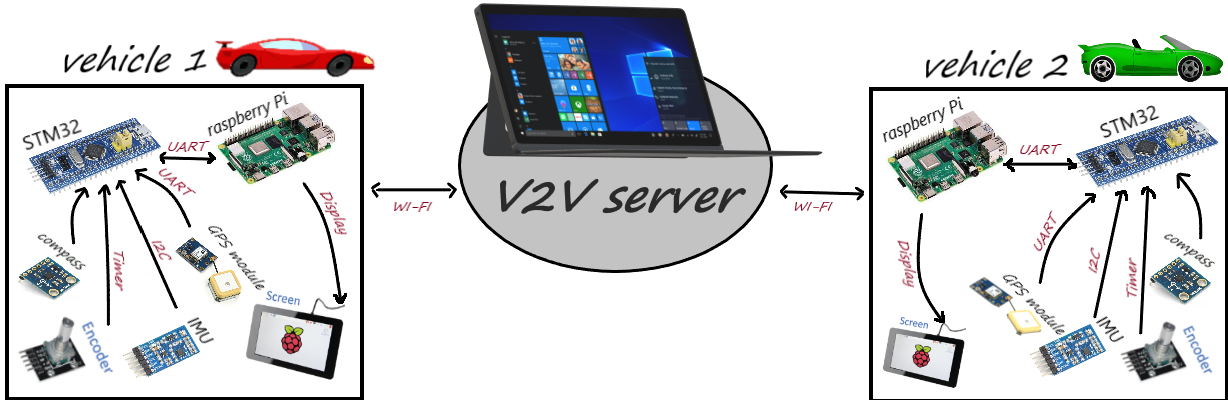
\includegraphics[width=\textwidth]{figure/2_1.png}
\caption{Block diagram of the project}
\label{fig:block-diagram}
\centering
\end{figure}

\subsection{Vehicle Unit}

The employed micro-controller, the STM32F103C8, handles data from the car connected to it as well as data from nearby cars. As a result, it must collect and analyze incoming data. In order to achieve this, as shown figure \ref{fig:vehicle-unit}, the STM is connected to:
\begin{itemize}
    \item \textbf{STM32F103C8: } It's the micro-controller which contains the analysis of the project. It is the processor of the project.
    \item \textbf{Raspberry Pi: }The Raspberry Pi serves as a link between a car and its neighboring cars. It communicates with STM using UART serial communication protocol and with the server via Wi-Fi. It also helps the user by providing a Graphical User Interface (GUI) system.
    \item \textbf{An inertial measurement unit (IMU): } The chosen IMU is GY-521 MPU6050 since it is based on Micro Electro-Mechanical Systems (MEMS) technology  which allows lower costs and low power requirements while ensuring performance. \newline
    The MPU-6050 sensor module measures acceleration, orientation, angular rates of the vehicle and reports it to the STM32 through an Inter-Integrated-Circuit (I2C) serial communication bus.
    \item \textbf{Inferred Rotary (IR) encoder: } The encoder which provides data on the rotating shaft's rotation angle and rotational speed (RPM).
    \item \textbf{Global Positioning System (GPS) module: }The GPS module, which is coupled to the STM32 through Universal asynchronous receiver-transmitter (UART) serial communication protocol, provides information about the car's location. \newline
    Note: Because of the weakness of GPS connection, it is replaced by Bluetooth module which receives the GPS data from mobile by Bluetooth and sends it to STM using UART.
    \item \textbf{compass module: } Compass provides STM with the angle between the vehicle and north direction.
    \item \textbf{Screen: } The screen is used to display the data for the user.
\end{itemize}

\begin{figure}
    \centering
    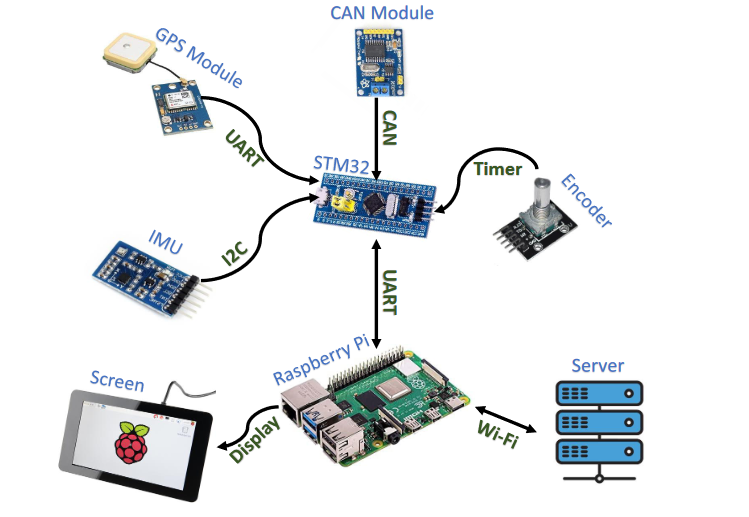
\includegraphics[width = \textwidth]{figure/2_1_1.PNG}
    
    \caption{Diagram for V2V vehicle unit}
    \label{fig:vehicle-unit}
\end{figure}

\newpage
\subsection{Server Unit}
The server used in that project is actually a laptop. All Raspberry Pi boards inside the system of V2V must be connected through Wi-Fi to the server in order to send and receive data in the form of JSON files anytime. \newline
 The server receives data from any connected vehicle and sends this data to all other connected cars. After receiving a JSON file, Raspberry Pi converts it into a string to be sent to the STM, by the same time, STM extracts data from the mentioned sensors and modules, and then it analyzes both data from its vehicle and from the neighboring vehicle and gives a warning message if an action must be taken to avoid a collision.\newline
 
 \section{Project Steps}
 This section will show an overview for the project steps that are followed, the details for each step will be discussed in separate chapters. \newline
 
 To build the vehicle unit, it is needed to follow these steps:
 \begin{enumerate}
     \item Drivers’ initialization: first of all, all drivers for STM protocols and peripherals are initialized, this step must be done before project implementation. The details will be discussed in chapter 4.
     \item Sensors and modules interfacing: After initialization of all needed drivers, sensors and modules are implemented and interfaced with STM to be ready to send and receive data. Details for each module and sensor interfacing are discussed in chapter 5.
     \item Data Analysis: After interfacing with sensors which provide STM with vehicle data, this data is analyzed for detecting any future accidents may be happened. Details for analysis and algorithms are discussed in chapter 6.
 \end{enumerate}
 
 
 The server unit is responsible for exchanging information between vehicles, the implementation steps are as follows:
 
 \begin{enumerate}
     \item Simplex System: a simple program is written to send the data in only one way.
     \item Duplex System: After ensuring that the simplex code works correctly, it is improved to be able to send and receive information.
     \item Multiple files: The program needs to be able to handle sending and receiving multiple files.
     \item Multiple clients: The Program has to handle more than one client.
     \item GUI: The server provided a simple GUI for administration.
\end{enumerate}
 After these steps, the server works properly as data is sent from one client to the server in JavaScript Object Notation (JSON) format, then the server sends it to other clients, these clients receive the data in JSON format, then it converts it into string to be sent to STM. Inner workings of the server will be discussed in chapter 7. \newline
 Now, both V2V unit and server unit are implemented separately, the next step would be to have them communicate with each other.
 
 Hardware implementation is discussed in chapter 8.
 
 
\chapter{Communication Protocols}
Before going deeply into details of the project, wired and wireless communication protocols have to be discussed since the project is considered as communication system, so this chapter shows how communication protocols are used in the project, and why was each one chosen. Wired communications that will be discussed are UART, I2C, and SPI, and these protocols are important to communicate between the prototype of the project and the sensors, CAN protocols is also discussed since it plays an important role in the modern cars. This chapter will also explain wireless communication protocols such as Wi-Fi and Bluetooth.

\section{Wired Communication Protocols}
Wired communication is an efficient method to communicate between nearby devices, thus the usage of wired communication appears in V2V vehicle unit since it helps to communicate between sensors/modules and the processor.
In this section UART, I2C, SPI, and CAN are discussed through the following points:
\begin{enumerate}
    \item Background
    \item Why it is being used?
    \item Interfacing
\end{enumerate}
\subsection{UART}
There was a time when keyboards, mouse, and printers all had large cords and clumsy connectors. These must be inserted into the computer with a screwdriver. To interact with computers, these devices used UART. Although USB has replaced these clumsy wires, UARTs are still used in Do It Yourself (DIY) electronics like the Raspberry Pi, Arduino, and other ubiquitous microcontrollers. It can be used to link Bluetooth and GPS modules together. \newline
Other communication protocols, such as SPI and I2C, use a different transfer methodology than UART. In a microcontroller, it is a physical circuit. It can also work on its own as an integrated circuit. The fact that UART only uses two wires to carry data is a huge advantage. \clearpage
\subsubsection{1. Background of UART}
\begin{wrapfigure}{r}{5cm}
    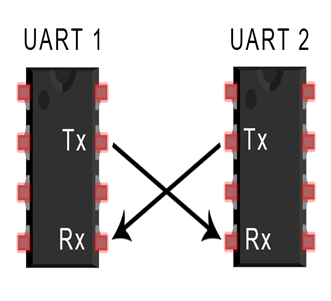
\includegraphics[width=0.25\textwidth]{figure/3_1.png}
    \caption{Connection between two devices using UART}
    \label{fig:connection-two-devices}
\end{wrapfigure}
Two UARTs communicate directly with each other in UART communication. The transmitting UART translates parallel data from a controlling device, such as a CPU, into serial data and sends it to the receiving UART, which then converts the serial data back into parallel data for the receiving device. To send data between two UARTs, only two wires are required. Data transfers from the transmitting UART's Tx pin to the receiving UART's Rx pin as shown in figure \ref{fig:connection-two-devices}.
\subsubsection{Transmitting and receiving serial data}
The transmitting UART takes bytes of data and transmits the bits in a sequential form. The second transmitter which is the receiver reassembles the bits into a complete byte. Serial transmission of data through a single wire is more cost-effective than parallel transmission through multiple wires. \newline
Simplex, full-duplex, or half-duplex communication between two UART devices is possible. Simplex communication is one-way communication in which the signal travels from one UART to the next. The receiving UART does not have the ability to send back signals. When both devices can transmit and receive data at the same time, it is called full-duplex. When devices communicate and receive data in half-duplex mode, they take turns transmitting and receiving data. \newline
\subsubsection{Steps of the UART transmission}
\begin{itemize}
    \item The transmitting UART receives data in parallel from the data bus.
    \item The transmitting UART adds the start bit, parity bit, and the stop bit(s) to the data frame.
    \item The entire packet is sent serially from the transmitting UART to the receiving UART. 
    \item The receiving UART samples the data line at the pre-configured baud rate.
    \item The receiving UART discards the start bit, parity bit, and stop bit from the data frame:
    \item The receiving UART converts the serial data back into parallel and transfers it to the data bus on the receiving end.
\end{itemize}
\clearpage
\subsubsection{Structure of a UART Protocol}
UART Packet as shown in figure \ref{fig:UART-packet} consists of 4 parts; start bit, data bit/s, parity bit/s, and stop bit/s.
\begin{figure}[h]
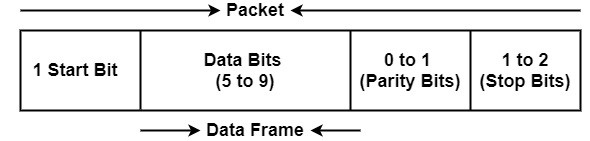
\includegraphics[width=\textwidth]{figure/3_2.jpg}
\caption{UART Packet}
\label{fig:UART-packet}
\centering
\end{figure}

\begin{itemize}
    \item \textbf{Start Bit: } Start-bit is also referred to as a synchronization bit that is located before the actual data. Usually, an inactive data transmission line is reserved at a high-voltage level. To start the data transmission, the UART transmission burden the data line from a high voltage level (1) to a low voltage level (0).
    \item \textbf{Stop Bit: } The Stop Bit is located at the ending of the data packet. Generally, this bit is 2-bits lengthy but commonly on bit only used. It can stop the broadcast, the UART maintains the data-line on high voltage.
    \item \textbf{Parity Bit: } The symmetry or oddness of a number is described by parity. The receiving UART uses the parity bit to determine if any data has changed during transmission. Electromagnetic radiation, mismatched baud rates, and long-distance data transfers can all alter bits. After reading the data frame, the receiving UART counts the number of bits with a value of 1 and determines whether the total is even or odd. The 1 bit in the data frame should amount to an even number if the parity bit is a 0 (even parity). The 1 bit in the data frame should amount to an odd number if the parity bit is a 1 (odd parity). The UART understands that the transmission was error-free when the parity bit matches the data. The UART knows that bits in the data frame have changed if the parity bit is a 0 and the total is odd; or if the parity bit is a 1 and the total is even. Briefly Parity bit allows the receiver to provide whether the collected record is right or not. It is a low-level fault checking system & parity bit is accessible in two ranges including Even Parity and Odd Parity.
    \item \textbf{Data Bits or Data Frame: } The data frame contains the actual data being transferred. It can be 5 bits up to 8 bits long if a parity bit is used. If no parity bit is used, the data frame can be 9 bits long. In most cases, the data is sent with the least significant bit first.
\end{itemize}

\subsubsection{2. Why UART is being used?}
\begin{enumerate}
    \item Low hardware complexity.
    \item Software addressing is not necessary because this connection is one to one between the two devices.
    \item It is often utilized in devices using 9 pin connectors due to its simplicity
\end{enumerate}

\subsubsection{3. Interfacing with UART}
In this project, UART protocol is used to interface between:
\begin{enumerate}
    \item Raspberry and STM: they transmit/receive data between them using UART protocol, Raspberry receives the output vehicle data from the STM to send them to the server, and it transmits the data came from Server to STM to pe processed and analyzed as will be shown in chapter 5.
    \item Bluetooth module and STM: In order to use GPS data, Bluetooth module is used since it connects to a mobile phone by Bluetooth using android application called “GPS share Data”, and in other side, it connects with STM and communicate with it by UART.
\end{enumerate}

Figure \ref{fig:interface-stm-rasp-bluetooth} shows how the connection is between STM and both the Bluetooth module and Raspberry; STM connects with Raspberry by UART2 whose pins are PA2 (Tx) and PA3 (Rx), PA2 is connected to Rx in Raspberry, and PA3 is connected to Tx, for Bluetooth module UART3 is used whose pins are PB10 (Tx) and PB11 (Rx), PB10 is connected to RX in the module, and PB11 is connected to Tx.

\begin{figure}[h]
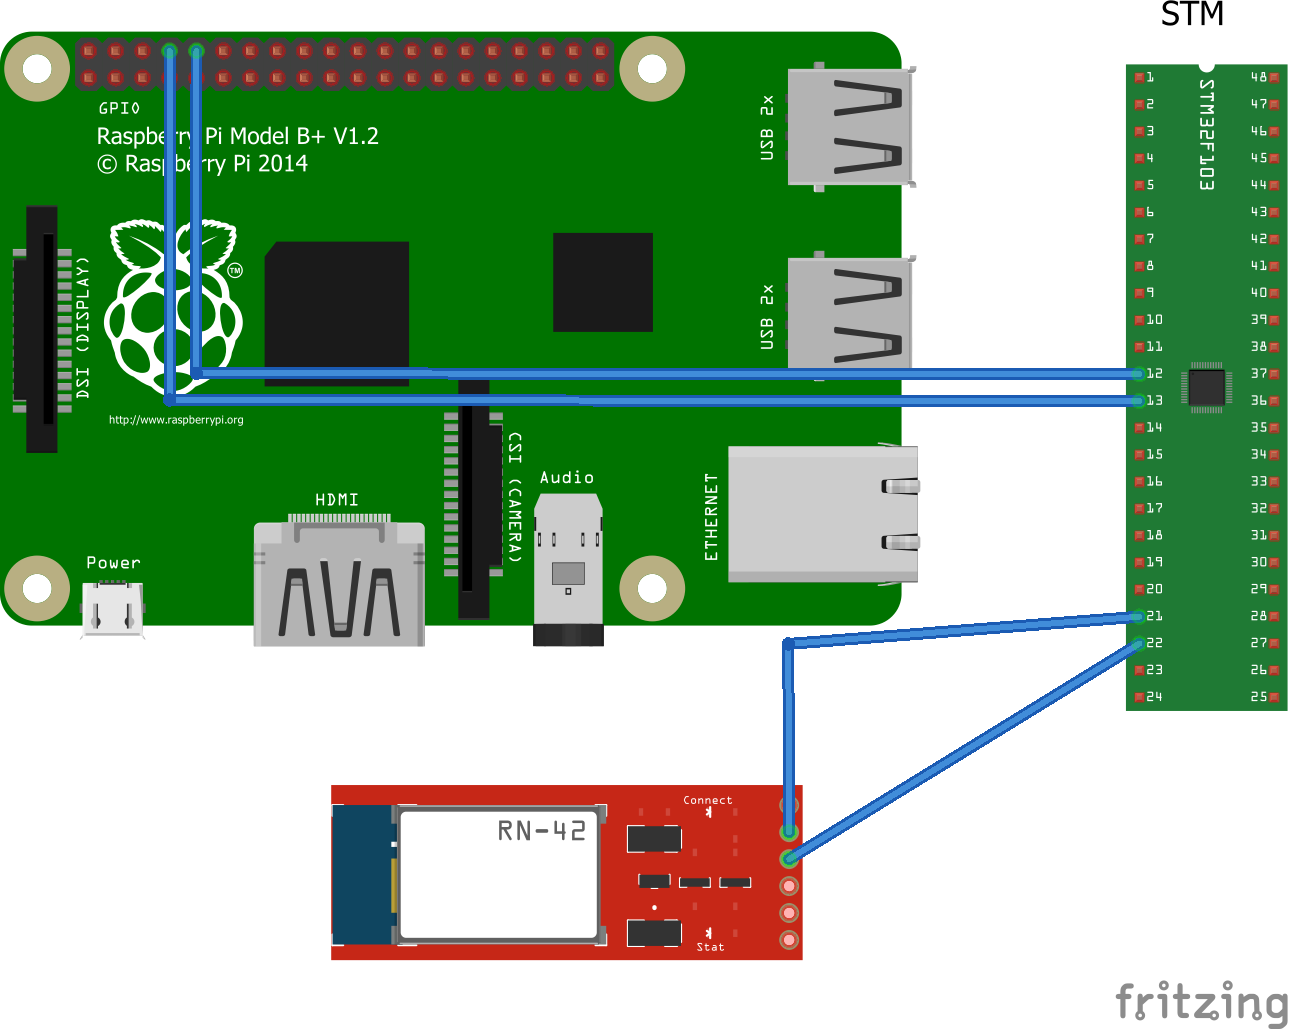
\includegraphics[width=\textwidth]{figure/3_3.png}
\caption{Intefcaing between STM and both Raspberry Pi and Bluetooth module}
\label{fig:interface-stm-rasp-bluetooth}
\centering
\end{figure}

\subsection{I2C}
Inter-Integrated Circuit is the acronym for it. It is a serial communication bus interface connection protocol used by devices. Philips Semiconductor created it at first in 1982. It has been a popular protocol recently for short-distance communication. It also goes by the name Two Wired Interface (TWI).

\subsubsection{1. Background of I2C}
Like UART communication, I2C only uses two wires to transmit data between devices as shown in figure \ref{fig:connectiong-i2c}. The main device is called Master (which is responsible for genrating a clock signal), and the second device is called Slave. Each device has two pins; SDA and SCL, SDA refers to select data, SCL refers to select clock line. The bus between SDAs pins is to transfer the data between two devices, and the bus between SCLs pin is to provide the clock for the slave device. 

\begin{figure}[h]
   \centering
    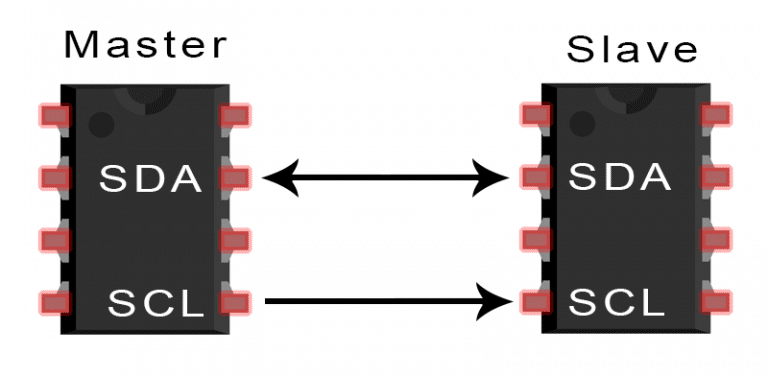
\includegraphics[width=0.5\textwidth]{figure/3_4.png}
    \caption{Connection between two devices using I2C}
    \label{fig:connectiong-i2c}
\end{figure}

\subsubsection{I2C Modes & Bus Speeds}
Originally, the I2C-bus was limited to 100 kbit/s operations. Over time there have been several additions to the specification so that there are now five operating speed categories. Standard-mode, Fast-mode (Fm), Fast-mode Plus (Fm+), and High-speed mode (Hs-mode) devices are downward compatible. This means any device may be operated at a lower bus speed. Ultra Fast-mode devices are not compatible with previous versions since the bus is unidirectional.
\begin{enumerate}
    \item Bidirectional bus:
    \begin{itemize}
        \item Standard-Mode (Sm), with a bit rate up to 100 kbit/s 
        \item Fast-Mode (Fm), with a bit rate up to 400 kbit/s
        \item Fast-Mode Plus (Fm+), with a bit rate up to 1 Mbit/s 
        \item High-speed Mode (Hs-mode), with a bit rate up to 3.4 Mbit/s. 
    \end{itemize}
    \item Unidirectional bus: 
    \begin{itemize}
        \item Ultra Fast-Mode (UFm), with a bit rate up to 5 Mbit/s 
    \end{itemize}
\end{enumerate}
Both SDA and SCL are bidirectional lines, connected to a positive supply voltage via a current source or pull-up resistor. When the bus is free, both lines are HIGH. The output stages of devices connected to the bus must have an open-drain or open-collector to perform the wired-AND function. \newline

\subsubsection{I2C working abstract}
With I2C, data is transferred in messages, Messages are broken up into frames of data. \newline
I2C message as shown in figure \ref{fig:i2c-message} has an address frame that contains the binary address of the slave, and one or more data frames that contain the data being transmitted. The message also includes start and stop conditions, read/write bits, and ACK/NACK bits between each data frame. \newline
\begin{figure}[h]
   \centering
    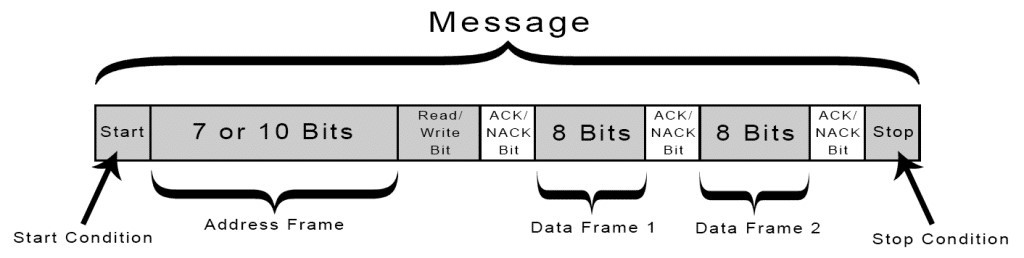
\includegraphics[width=.5\textwidth]{figure/3_5.jpg}
    \caption{I2C Message}
    \label{fig:i2c-message}
\end{figure}

\begin{itemize}
    \item \textbf{Start Condition: } The SDA line switches from a high voltage level to a low voltage level before the SCL line switches from high to low.
    \item \textbf{Stop Condition: } The SDA line switches from a low voltage level to a high voltage level after the SCL line switches from low to high. 
    \item \textbf{Address Frame: }  A 7- or 10-bit sequence unique to each slave that identifies the slave when the master wants to talk to it. 
    \item \textbf{Read/Write Bit: }  A single bit specifying whether the master is sending data to the slave (low voltage level) or requesting data from it (high voltage level). 
    \item \textbf{ACK/NACK Bit: } Each frame in a message is followed by an acknowledge/no-acknowledge bit. If an address frame or data frame was successfully received, an ACK bit is returned to the sender from the receiving device. 
\end{itemize}

\subsubsection{2. Why I2C is being used?}
\begin{enumerate}
    \item Can be configured in multi-master mode.
    \item Complexity is reduced because it uses only 2 bi-directional lines (unlike SPI Communication).
    \item Cost-efficient.
    \item It uses ACK/NACK feature due to which it has improved error handling capabilities.
\end{enumerate}

\subsubsection{3. Interfacing with I2C}
In the project, sensors that are used is working with I2C, so I2C plays an important rule for communicating between STM and sensors. \newline
The advantage of I2C that all sensors can use only one I2C by acting as slaves and STM acts as the master, I2C 1 is used and sensors were rotary shaft encoder and compass. \newline

\subsection{SPI}
Serial Peripheral Interface, or SPI, is a communication protocol that is widely used in microcontroller systems. SPI is used in devices such as sensors, liquid crystal displays, and memory cards. It is faster than both UART and I2C, but it has drawbacks as well.
\subsubsection{1. Background of SPI}
\begin{wrapfigure}{r}{5cm}
    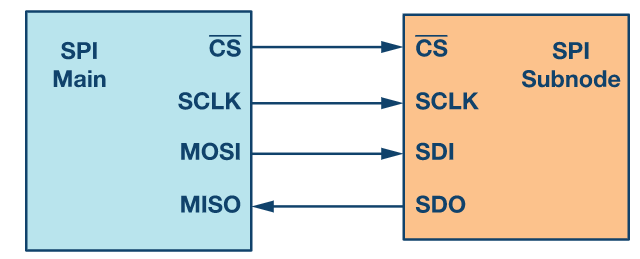
\includegraphics[width=0.5\textwidth]{figure/3_6.png}
    \caption{Connection between two devices using SPI}
    \label{fig:connection-spi}
\end{wrapfigure}
One of the most popular interfaces between micro-controllers and peripheral ICs, including sensors, ADCs, DACs, shift registers, SRAM, and others, is serial peripheral interface (SPI). The SPI interface is briefly explained. SPI is a main-subnode-based, synchronous, full-duplex interface. On the rising or falling clock edge, the data from the main node or the sub-node are synchronized. Data can be transmitted simultaneously by the main and sub-node. Both a 3-wire and a 4-wire SPI interface are available. When using more than sub-node, the forth pin is used since it is responsible for chip select as shown in figure \ref{fig:connection-spi}.\newline
The main must activate the CS signal, send the clock signal, and choose the sub-node before SPI communication can start. To pick the sub-node, the main must provide a logic 0 on the chip select signal, which is often an active low signal. Full-duplex SPI allows for simultaneous data transmission between the main and sub-node via the MOSI and MISO lines, respectively. Data is concurrently sent (shifted out serially onto the MOSI/SDO bus during SPI communication) and received (sampled or read in from the bus, MISO/SDI) during SPI communication. \newline
The shifting and sampling of the data are synchronized by the edge of the serial clock. The SPI interface gives the user the freedom to choose whether to sample and/or shift the data on the rising or falling edge of the clock. To find out how many data bits are sent over the SPI interface, please consult the device data sheet.

\subsubsection{SPI Pins}
SPI uses three pins for communication:
 MOSI, MISO and SCLK. MOSI is short for 
Master-Out-Slave-In and MISO stands for 
Master-In-Slave-Out. This shows that SPI
 uses master-slave scheme and operates 
at full duplex (simultaneous two-way communication). \newline
The SPI parameters, such as data rate, bit order, and mode, are set by the master device. The data rate is the SPI transmission speed, which is determined by the microcontroller's clock speed. The bit order specifies whether the first bit out is the rightmost (LSB) or leftmost (MSB). The next part delves deeper into the topic of mode. There can only be one master device, and the number of slaves is proportional to the number of Slave Select (SS) pins on the master device. When a master wishes to converse with a slave, the SS line to that slave is set to low, while the rest of the lines are set to high. After then, the data is read on the MOSI line, and the slave responds on the MISO line. Slaves have no direct communication with their fellow slaves. Pull-up resistors on SS pins are a solid design technique for efficiently isolating slave devices from one another’s is a de facto standard, albeit a sloppy one. As a result, device makers may implement the protocol in a variety of ways. It's a good idea to read the gadget datasheet beforehand. \newline

\subsubsection{SPI Interface}
A basic SPI connection uses the serial clock (SCK), Master Out Slave In (MOSI), Master in Slave Out (MISO), and Slave Select (SS) lines to link a master to slaves, as shown in figure \ref{fig:spi-integration}. Slaves can share the SCK, MOSI, and MISO signals, but each slave has its own SS line.
\begin{figure}[h]
   \centering
    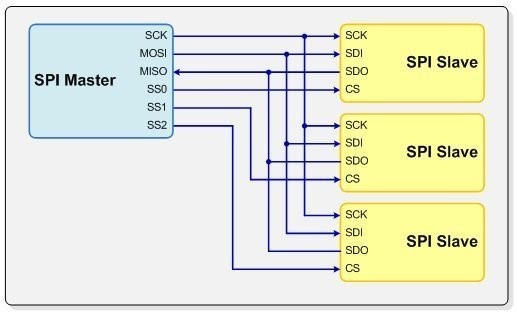
\includegraphics[width=.45\textwidth]{figure/3_7.jpg}
    \caption{SPI bus configuration with multiple slaves}
    \label{fig:spi-integration}
\end{figure}

\subsubsection{SPI Mode: Polarity and Clock Phase}
The SPI interface has no data exchange protocol, which reduces overhead and allows for high-speed data streaming. As shown in figure \ref{fig:spi-timing}, clock polarity (CPOL) and clock phase (CPHA) can be set to ‘0’ or ‘1’ to create four distinct modes for communication between master and slave.
\begin{figure}[h]
   \centering
    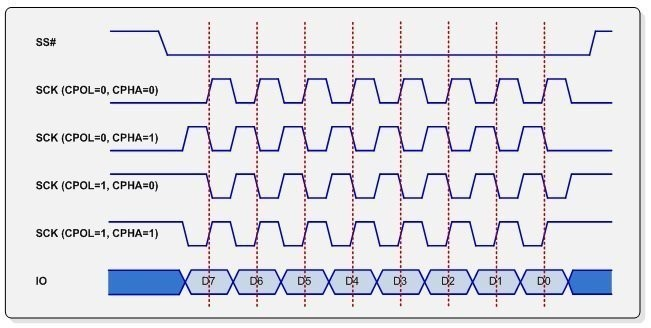
\includegraphics[width=\textwidth]{figure/3_8.jpg}
    \caption{SPI bus timing}
    \label{fig:spi-timing}
\end{figure}

As shown in figure \ref{fig:spi-modes}, Data is sampled at the leading rising edge of the clock if CPOL and CPHA are both ‘0’ (designated as Mode 0). SPI bus slave communication in mode 0 is by far the most prevalent. Data is sampled at the leading falling edge of the clock if CPOL is ‘1’ and CPHA is ‘0’ (Mode 2). Similarly, data sampled on the trailing falling edge with CPOL = ‘0’ and CPHA = ‘1’ (Mode 1), and data sampled on the trailing rising edge with CPOL = ‘1’ and CPHA = ‘1’ (Mode 3).

\begin{figure}[h]
   \centering
    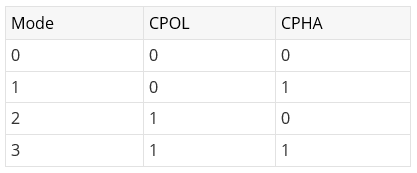
\includegraphics[width=\textwidth]{figure/3_9.PNG}
    \caption{SPI modes}
    \label{fig:spi-modes}
\end{figure}


\subsubsection{2. Why SPI is being used}
\begin{enumerate}
    \item Full duplex communication is supported.
    \item Because SPI uses a push-pull architecture, it can accommodate faster data speeds and longer distances.
    \item In comparison to I2C interface, it uses less power.
    \item Data can be transferred at high speed in tens of MHz.
\end{enumerate}

\subsubsection{3. Interfacing with SPI}
Although the ease of this protocol, it has a small role in the project since the used sensors and modules communicate with UART and I2C, so SPI driver is interacted with CAN module and raspberry pi to send and receive some data which will may need to display for the user.

\subsection{CAN}
Modern cars may feature up to 100 sensors and ECUs that must communicate and interact with one another in order to transfer data and monitor the vehicle's state. Microcontrollers and ECUs are increasing in number as more features are introduced to cars, such as smart car systems, autonomous driving systems, and V2X systems. Sensor devices provide information such as speed, position, and heat. As the information is vital to minimize accidents and traffic concerns, the Controller Area Network (CAN)communication protocol has been determined to be dependable to handle the communication with the lowest potential error. The Controller Area Network (CAN) standard is used to allow microcontrollers and devices in a vehicle to interact without the usage of a host computer. In many applications where several remote MCUs and sensors must interact with one another, such as industrial automation or robotics, the CAN bus provides a good communication protocol.

\subsubsection{1. Background of CAN}
The CAN bus was developed by BOSCH (1) as a multi-master, message broadcast system that specifies a maximum signaling rate of 1 megabit per second (bps). Unlike a traditional network such as USB or Ethernet, CAN does not send large blocks of data point-to-point from node A to node B under the supervision of a central bus master. In a CAN network, many short messages like temperature or RPM are broadcast to the entire network, which provides for data consistency in every node of the system. Once CAN basics such as message format, message identifiers, and bit-wise arbitration -- a major benefit of the CAN signaling scheme are explained, a CAN bus implementation is examined, typical waveforms presented, and transceiver features examined.

\subsubsection{The CAN Standard}
CAN is an International Standardization Organization (ISO) defined serial communications bus originally developed for the automotive industry to replace the complex wiring harness with a two-wire bus. The specification calls for high immunity to electrical interference and the ability to self-diagnose and repair data errors. These features have led to CAN’s popularity in a variety of industries including building automation, medical, and manufacturing. The CAN communications protocol, ISO-11898: 2003, describes how information is passed between devices on a network and conforms to the Open Systems Interconnection (OSI) model that is defined in terms of layers. Actual communication between devices connected by the physical medium is defined by the physical layer of the model. The ISO 11898 architecture defines the lowest two layers of the seven-layer OSI/ISO model as the data-link layer and physical layer in figure \ref{fig:iso-standard}.

\begin{figure}[h]
   \centering
    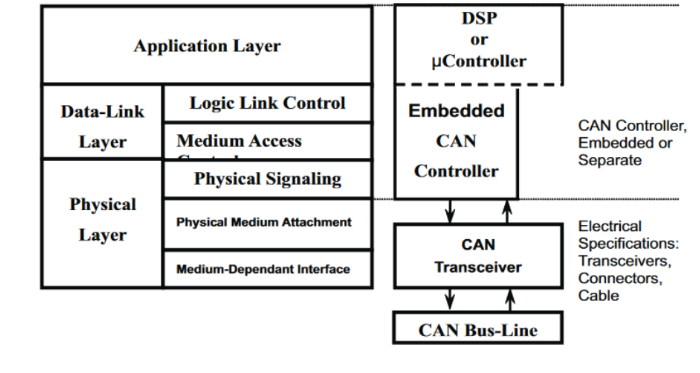
\includegraphics[width=\textwidth]{figure/3_10.png}
    \caption{The Layered ISO 11898 Standard Architecture. }
    \label{fig:iso-standard}
\end{figure}

\subsubsection{The Bit Fields of Standard CAN}
\begin{itemize}
    \item SOF - Start of Frame.
    \item 11-bit Identifier - establishes the priority of the message.
    \item  The lower the binary, the higher its priority.
    \item RTR - Remote Transmission Request is dominant
 when information is required from another node.
    \item IDE - Dominant single identifier extension bit means
 that a standard CAN identifier with no extension is being transmitted. 
 \item R0 – Reserved bit. 
 \item DLC – The 4-bit data length code. 
 \item Data – Up to 64 bits.
 \item CRC – The 16-bit cyclic redundancy check.
 \item ACK - Acknowledgment bit.
 \item EOF - End of Frame. 
 \item IFS – This 7-bit interframe space (IFS) contains the time 
required by the controller to move a correctly received frame 
to its proper position in a message buffer area.
\end{itemize}

\subsubsection{2. Why CAN is being used?}
A Controller Area Network (CAN) is ideally suitable for industrial communication protocols. Its cost, performance, and upgradeability provide high flexibility in system design. So, there is many advantages of CAN protocol.

\begin{enumerate}
    \item Low Cost
    \item Built-in Error Detection
    \item Robustness
    \item Speed
    \item Flexibility
\end{enumerate}

\subsubsection{3. Interfacing with CAN}
To interface between STM and can module, CAN bus must to implemented and integrated between them, and in order to make use of raspberry pi features, CAN module connects with raspberry using SPI protocol as shown in figure \ref{fig:interface-can}.
\begin{figure}[h]
   \centering
    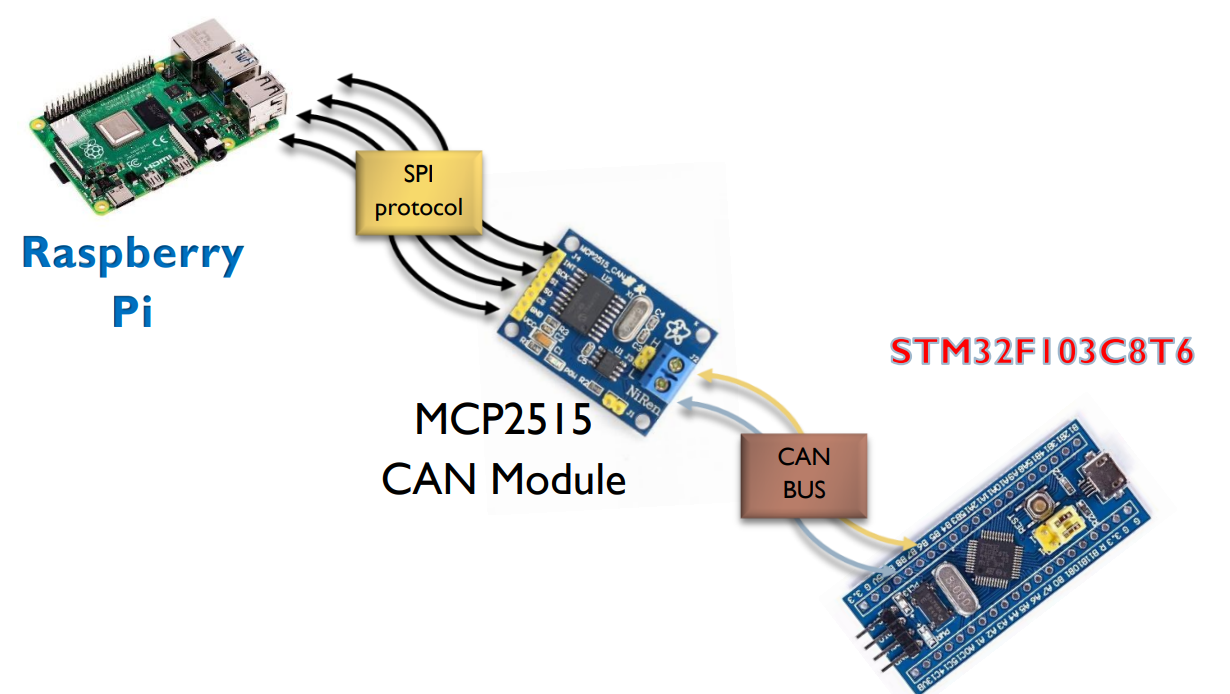
\includegraphics[width=\textwidth]{figure/3_11.png}
    \caption{Interfacing RP, STM32F103, and MCP2515 CAN Bus Module}
    \label{fig:interface-can}
\end{figure}

\section{Wireless Communication Protocols}
Wireless communication is needed to be able for V2V unit to communicate with the server and the mobile. In the following, Bluetooth and Wi-Fi will be discussed and how they are used in the project.

\subsection{Bluetooth}
Bluetooth is a short-range wireless technology; it can be used to exchange data between two devices in a short distance, so Bluetooth communication is a suitable choice to communicate between a mobile and the project. \newline
As discussed before, Bluetooth module was used to communicate with STM and in other side, it communicates with a mobile phone to give it all GPS data which includes longitude, latitude, and time. There are a lot of mobile software application that handle sharing GPS data from the mobile to any device has a Bluetooth module. \newline

Bluetooth is also used to communicate between the car prototype and the mobile to control the car motion remotely, it will be discussed in details in chapter 8.

\subsection{Wi-Fi}
Wi-Fi is a family of wireless network protocols, based on IEEE 802.11, Wi-Fi is suitable for wide range communication in a local area, so it is used for communicate between the vehicles and the server. \newline
To implement the connection, LAN network is integrated to connect a group of peripheral devices that share a common communications line or wireless link to a server within a distinct geographic area. \newline
Mentioned peripheral device in the project is Raspberry pi for each V2V unit since it has a Wi-Fi protocol. Details of this communication is discussed in chapter 6.


\chapter{Software Drivers Initialization}

This chapter discuss the peripherals of the STM either input or communication protocols. A driver is defined as a group of function that are written to do certain tasks of the peripheral that the driver is written for.
STM Cube Software saves times writing drivers with a very high quality automatic help instead of writing everything manually. The generated drivers are available within made libraries known as \textbf{HAL libraries}.
The objective of this chapter is to through the features of the program then before each peripheral how the HAL was used and how the configuration was made.

\section{STM Cube Software}

STM Cube program is a graphical software configuration tool, it generates a source code for the user in C language which includes drivers and interfaces that are implemented in a standard library called Hardware Abstraction Layer or HAL library.\\ The HAL library is complementary and covers a wide range of requirements for the user since it offers high-level and feature-oriented Application Programming Interface (APIs) with a high probability level.\\

\emph{Peripheral drivers APIs are organized in four groups:}
\clearpage
\begin{table}[]
\centering
\def\arraystretch{1.5}
\begin{tabular}{| c | c |}
\hline
\cellcolor[HTML]{B4C6E7}Group & \cellcolor[HTML]{B4C6E7}Examples\\
\hline
Initialization and deinitialization group & \begin{tabular}[c]{@{}l@{}}\textbf{HAL\_GPIO\_Init()}\\    \\ \textbf{HAL\_GPIO\_DeInit()}\end{tabular}                      \\ \hline
Process operation & \begin{tabular}[c]{@{}l@{}}\textbf{HAL\_UART\_Receive()}\\    \\ \textbf{HAL\_UART\_Transmit()}\\    \\ \textbf{HAL\_UART\_Transmit\_IT()}\end{tabular}   \\ \hline
Peripherical subsystem configuration      & \begin{tabular}[c]{@{}l@{}}\textbf{HAL\_ADC\_ConfigChannel()}\\    \\ \textbf{HAL\_RTC\_SetAlarm()}\end{tabular}                                 \\ \hline
Peripherical GetState and GetError        & \begin{tabular}[c]{@{}l@{}}\textbf{HAL\_I2C\_GetState()}\\    \\ \textbf{HAL\_I2C\_GetError()}\end{tabular}  \\ \hline                                    
\end{tabular}
\end{table}

\section{STM32 peripherals}
The need peripherals in the project are: General Purpose Input Output, Timers, Interrupts and, Communication Peripherals.
\subsection{General Purpose Input Output}
The driver for the General Purpose Input Output of GPIO is critical for any embedded project, STM Cube helps generating the needed configuration by selection of which pins are either input or output and specify whether the pin needs to be normally pulled up or down. When opening the program one should choose the appropriate micro-controller in this case it’s the STM32f103C8.\\
Modifications for either input or output can be done using the menu on the left or with the help of the schematic of the micro-controller which appears in the middle of the window as shown in figure \ref{fig:gpio-config}.\\
\clearpage
\begin{figure}[h]
   \centering
    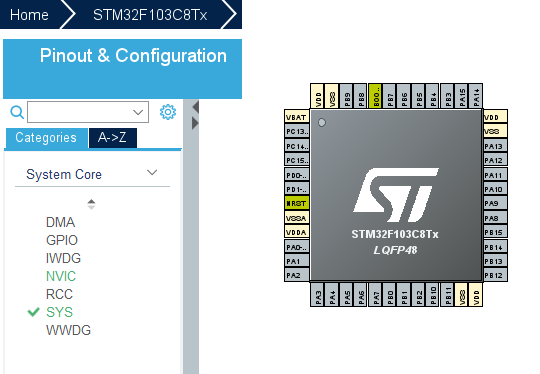
\includegraphics[width=\textwidth]{figure/4_1.png}
    \caption{GPIO configuration screen in STM Cube software}
    \label{fig:gpio-config}
\end{figure}

The GPIO driver provides many functions but the main ones used in this project:
\begin{enumerate}
    \item \textbf{HAL\_GPIO\_Init():} within the Main by default when performing the configuration and its purpose is to initialize the GPIO. A missing Init function would errors in case of the use of another GPIO function.
    \item \textbf{HAL\_delay():} responsible for delays between two commands and its argument is time measured in milliseconds.
    \item \textbf{HAL\_GPIO\_Write\_Pin():} used to output either HIGH or LOW for any pin already configured as output taking arguments of the port and the pin.
    \item \textbf{HAL\_GPIO\_Read\_Pin():} returns the value of a pin configured as input and takes the arguments as the port and the pin.
\end{enumerate}

\subsection{Timers}

An important peripheral acting as a clock, it’s indispensable to measure time and count values to give the needed output.In case of measuring the speed of the vehicle’s wheel the objective is to count the number of revolutions in a certain period, this is where the timer comes in.\\


Four timers are available each one has four channels which gives the possibility for 16 different timer dependant applications if the applications were chosen carefully to avoid conflict with the registers use. Each channel has a number of modes its uses will become apparent in the upcoming chapter. \\To activate the timer modifications have to be preformed on the RCC which is the processor’s clock. One of the advantages of using the HAL is that it generates settings for the RCC.\\

Going over the clock configuration in the program, which allows to set the clock, the desired frequency and whether to use internal or external clock as shown in  \ref{fig:timer-config}. Beware that the maximum for the STM is 72MHz and to reach it there would be a need for an external clock which is why the program gives you options to select from and values to change to reach the intended values as shown in figure \ref{fig:clock-config}.\\
\begin{figure}[h]
   \centering
    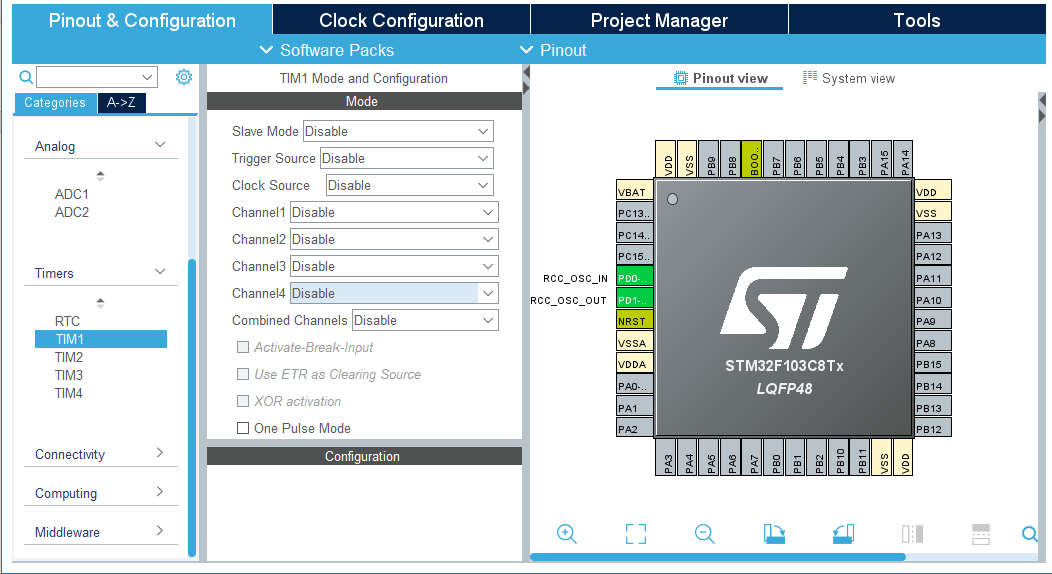
\includegraphics[width=.75\textwidth]{figure/4_2.png}
    \caption{Timer configuration screen in STM Cube software}
    \label{fig:timer-config}
\end{figure}
\begin{figure}[h]
   \centering
    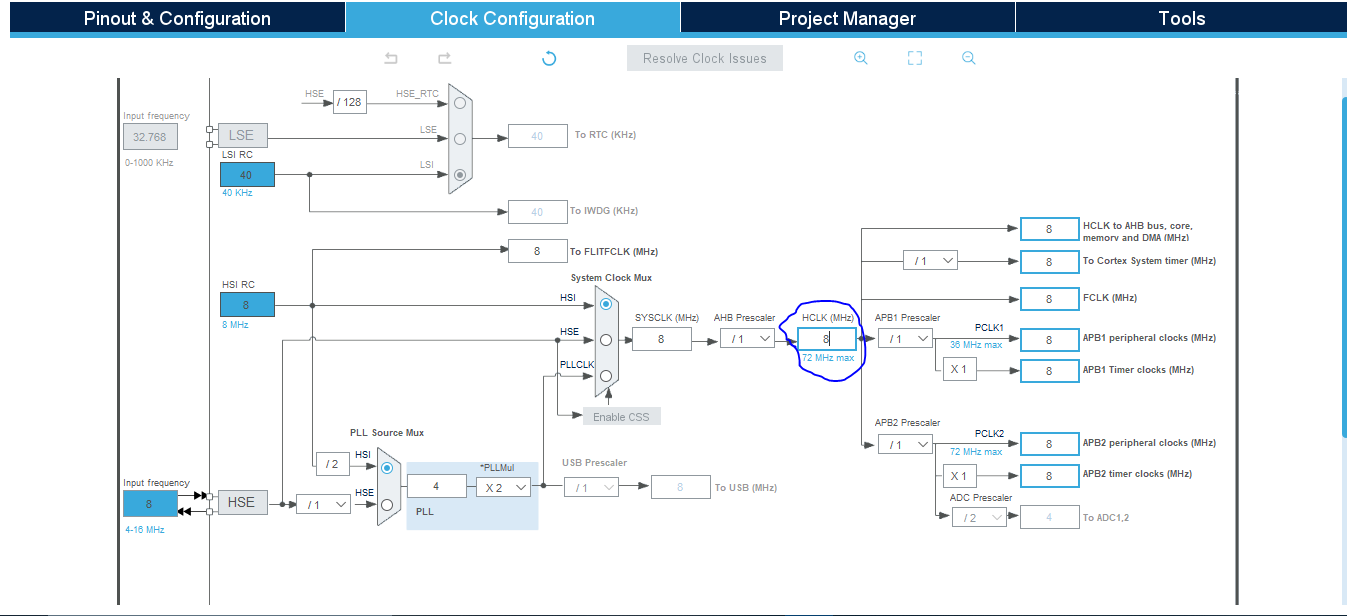
\includegraphics[width=.75\textwidth]{figure/4_3.png}
    \caption{Clock configuration screen in STM Cube software}
    \label{fig:clock-config}
\end{figure}

\clearpage

For the available functions provided by the HAL that are needed in the project:
\begin{enumerate}
    \item \textbf{MX\_TIMx\_Init():} written by default in the main to initiliaze the intended timers where the x is replaced by the number of the used timer.
    \item \textbf{HAL\_ROTARY\_Start():} used in the encoder mode which needs two channels per timer one internal and the second for the encoder.
\end{enumerate}

\subsection{Interrupts}

An important concept to understand is Nested Vector Interrupt Control (NVIC) which is available for some peripherals. If NVIC is enabled the HAL provides more functions for the intended peripheral such that the interrupt can be enabled with it. This is useful for the UART and the I2C.
The program also helps you organize each process that has its interrupt enabled by setting priority for each one. In case of two interrupts being activated at the same time the microcontroller will respond to the higher priority.\\
Some peripherals can be run in two possible methods, the first one called polling which activates the blocking mode. This method can cost more time however it is needed for certain tasks to be further explored in the upcoming chapter. The second method is the interrupt, in this case the process runs in the background meaning that it won’t be run unless the interrupt is activated which gives faster activation.\\
Additionally the STM also provides the Direct Memory Access Method but it wasn’t needed in the project.\\


\subsection{Universal asynchronous receiver-transmitter (UART)}

Universal asynchronous receiver-transmitter (UART) is indispensable part as it is the method of communication between the Raspberry Pi and the microcontroller.

\subsubsection{UART in the HAL library}
HAL library provides three methods can be used for UART communication
\begin{enumerate}
    \item Polling method: This method transmits/receives data in blocking mode and it will not allow any other operation to be implemented until the transmission/receive is done or time out occurred.
    \item Interrupt method: In this method, data transmission takes place in background or in non-blocking mode, When transmission is complete,\\ \textbf{HAL\_UART\_TxCpltCallback()} function is called, and the user can write inside this functions the instructions they need.
    \item DMA method: DMA works somewhat same as interrupt, meaning that data transfer is in non-blocking mode.\\

\end{enumerate}

In DMA, when half of the data get transferred, a half transfer get triggered and \textbf{HAL\_UART\_TxHalfCpltCallback()} function is called. The idea behind using DMA is when the second half of the data is being transferred, new data can be written in the first half section.

\subsubsection{Handle structure}

Handles contain information about related periphery and they are defined as global variables in the main file.\\

\emph{Handle structure consists of certain data types, some of them shown in the table below}

\begin{table}[h]
\def\arraystretch{1.5}
\centering
\begin{tabular}{| c | c |}
\hline
\cellcolor[HTML]{B4C6E7}Data   Type & \cellcolor[HTML]{B4C6E7}Value\\
Instance                            & USART1 or USART2\\
\hline
Baud rate                           & 9600 or 115200 \\
\hline
Status                              & Ready, Busy, and Error \\
\hline
Lock                                & Lock or unlock\\
\hline
Internal Status                     & TX or RX \\
\hline
*hdma tx pointer                    & DMA TX handler\\
\hline
*hdma rx pointer                    & DMA RX handler\\
\hline

\end{tabular}
\end{table}

i.e., when data is transmitted, first information is stored into the handler (how many bits to send, what is the baud rate, what is the status…etc.), after that they are sent to UART periphery. Not only the HAL function provides handler for USART1 and USART2, but also it provides handlers when the DMA method is used, and they are linked with UART handler together as shown below.\\

\subsubsection{HAL UART functions}

HAL functions are implemented to help the user to use the UART by the method they chose as well it provides system functions to initialize and set the UART, so the user does not need to initialize the registers and set the values for the UART.


\begin{enumerate}
    \item Initialization Functions:
    \begin{enumerate}
        \item \textbf{MX\_UART\_Init():}\\
        This function takes void arguement and returns void, it is called automatically in the code generated from STMCube, its functionalities are:
        \begin{itemize}
            \item Store UART parameters into initialize structure in UART handler
            \item Call \textbf{HAL\_UART\_Init()}
        \end{itemize}
        
        \item \textbf{HAL\_UART\_Init():}\\
        This function takes address of handler structure value and the returns void, it is called inside the \textbf{MX\_UART\_Init()}, its functionalities are:
        \begin{itemize}
            \item Store initialization structure (handler) into UART registers.
            \item Call \textbf{HAL\_UART\_MspInit()}
        \end{itemize}
        
        \item \textbf{HAL\_UART\_MspInit():}
        This function takes handler structure value and the returns void, its function is to initialize the GPIO parameters (pull up, speed, mode, pin state...etc.).\\
        
     
        \emph{Figure \ref{fig:init-flow-chart} summarizes initialization functions}
        
        \begin{figure}[h]
        \centering
        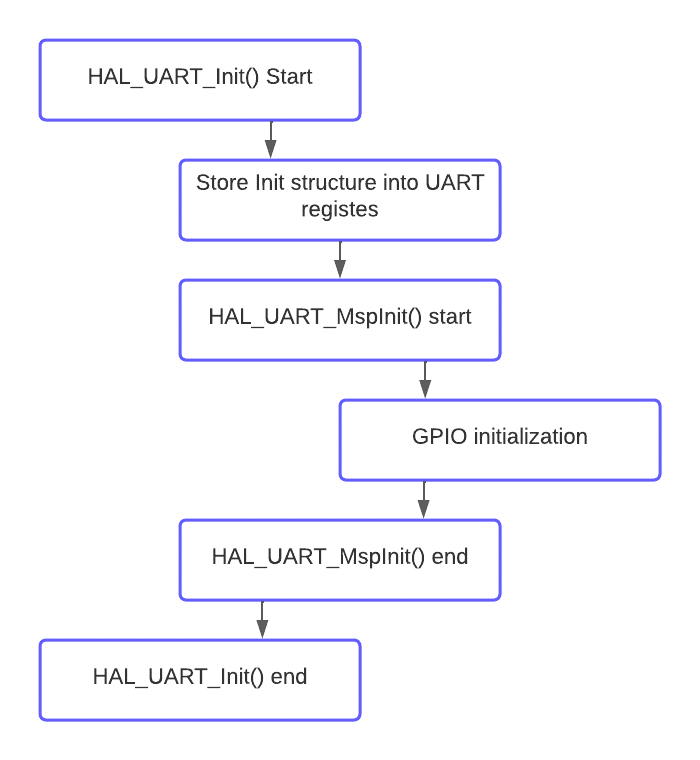
\includegraphics[width=.75\textwidth]{figure/4_4.png}
        \caption{Initialization functions flow chart}
        \label{fig:init-flow-chart}
    \end{figure}

    \clearpage
    \end{enumerate}
    \item User Functions:
    HAL library provides some functions for the three methods
    \begin{enumerate}
        \item Polling Method:
        HAL functions handle blocking polling processes, the functions that can be used are:
        \begin{itemize}
            \item \textbf{HAL\_UART\_Transmit():} This function takes four arguments; handler structure, buffer for data to be transmitted, size of buffer, and the time for transmitting and it returns HAL\_status prototype which it can be HAL\_OK, HAL\_BUSY, and HAL\_ERROR.
            \item \textbf{HAL\_UART\_Receive():} This function takes four arguments; handler structure, buffer for data to be received, size of buffer, and the time for receiving and it returns HAL\_status prototype which it can be HAL\_OK, HAL\_BUSY, and HAL\_ERROR.\\
            
            
        \end{itemize}
        \emph{Figure \ref{fig:user-func-flow-chart} shows a flow chart for which is inside the receive function (and the same in transmit function).}
            \begin{figure}[h]
            \centering
            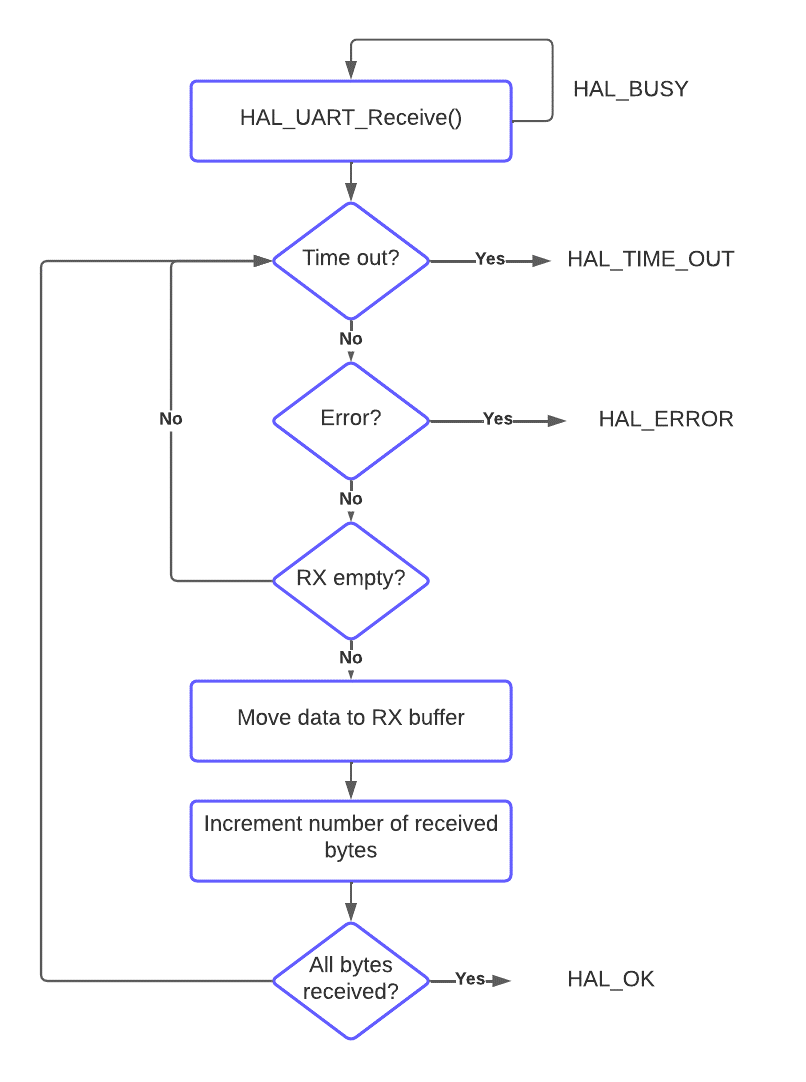
\includegraphics[width=.65\textwidth]{figure/4_5.png}
            \caption{User functions flow chart}
            \label{fig:user-func-flow-chart}
            \end{figure}

        \clearpage
        \item Interrupt Method:
        Interrupt method is used to solve the problem of blocking mode to make the process complete executing its processes and UART will be in the background (non-blocking mode).\\
        In this method, \textbf{HAL\_UART\_MspInit()} will call two new functions to handle the interrupt:
        
        \begin{itemize}
            \item \textbf{HAL\_NVIC\_SetPriority():} This function is to set the priority of the UART interrupt whether it has a low priority or high. NVIC stands to Nested Vector Interrupt Controller.
            \item \textbf{HAL\_NVIC\_EnableIRQ():} This function is to enable the handler of the interrupt. IRQ stands for interrupt request.
        \end{itemize}
        
        \emph{Also, HAL library provides other functions to be called when performs the receive/transmit functions:}
        \begin{itemize}
            \item \textbf{HAL\_UART\_Transmit\_IT():} “IT” stands for interrupt, this function takes three arguments; handler structure, buffer for data to be transmitted, and size of buffer, and it returns HAL\_status prototype which it can be HAL\_OK or HAL\_ERROR. 
            \item \textbf{HAL\_UART\_Receive\_IT():} This function takes three arguments; handler structure, buffer for data to be received, and size of buffer, and it returns \textbf{HAL\_status} prototype which it can be HAL\_OK or HAL\_ERROR.
            \item \textbf{HAL\_UART\_IRQHandler():} This function is to handle the interrupt request of the UART inside the system.
            \item \textbf{HAL\_UART\_RXcpltCallback():} “cpltCallback” stands for complete callback, this function is automatically called when \textbf{HAL\_UART\_Receive\_IT()} finishes its code, the user can write inside this function since it is used to be such as a flag for the ending of the receiving. 
            \item \textbf{HAL\_UART\_TXcpltCallback():} This function is automatically called when \textbf{HAL\_UART\_Transmit\_IT()} finishes its code, the user can write inside this function since it is used to be such as a flag for the ending of the transmission.

        \end{itemize}
        \clearpage
        \emph{Figure \ref{fig:interrupt-flow-chart} shows a flow chart for which is inside the interrupt receive function (and the same in transmit function).}\\
             \begin{figure}[h]
            \centering
            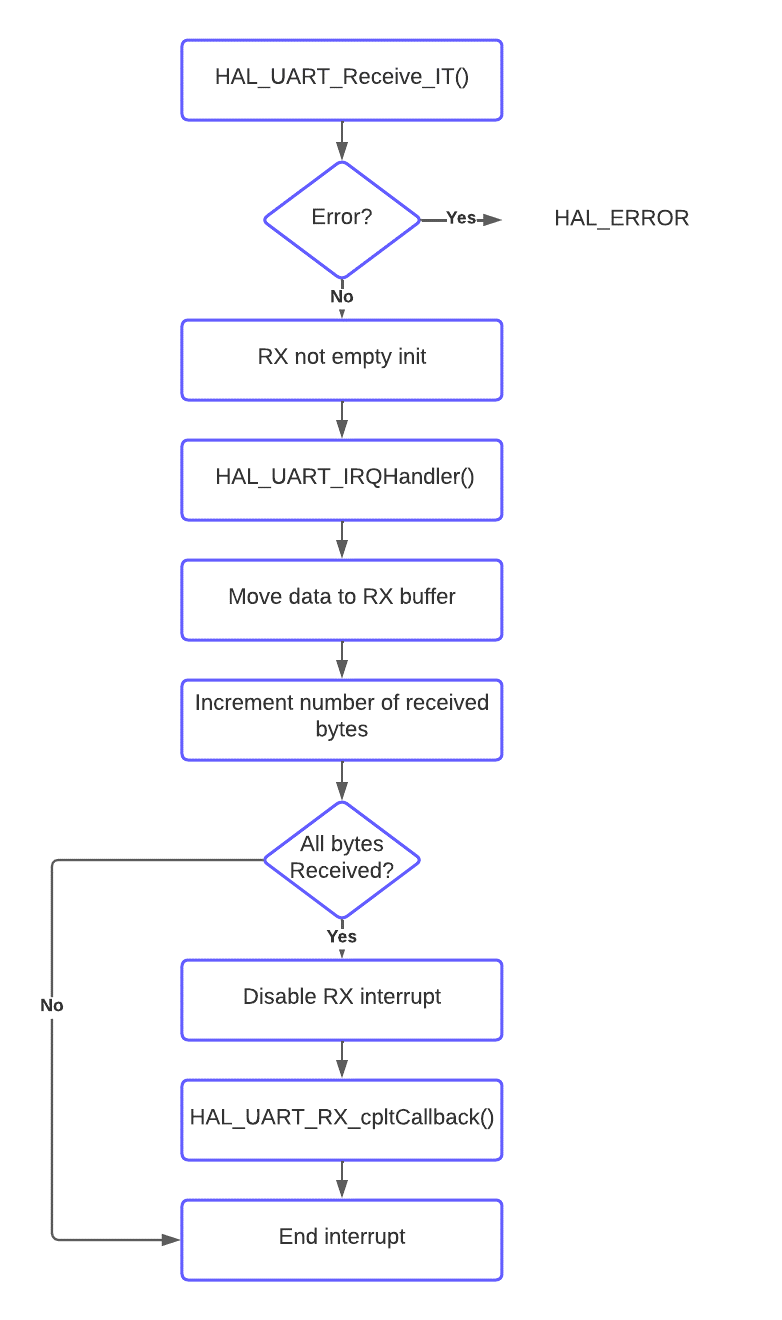
\includegraphics[width=.65\textwidth]{figure/4_6.png}
            \caption{Interrupt functions flow chart}
            \label{fig:interrupt-flow-chart}
            \end{figure}
       
    \end{enumerate}
\end{enumerate}

\subsection{Inter Integrated Circuit (I2C)}
 I2C is the method for communication between the micro-controller and some senors (IMU and Compass).\\
 
 Like UART, HAL library provides three methods that can be used for I2C communication
 \begin{enumerate}
     \item \textbf{I2C With Polling: }The first and the easiest way to do anything in embedded software is just to poll for the hardware
resource until it’s ready to move on to the next step in your program instructions. However, it’s

the least efficient way to do things and the CPU will end up wasting so much time in a “busy-
waiting” state.

It’s the same thing for both transmission and reception. You just wait until the current byte of data
to be transmitted so you can start the next one and so on.
     \item \textbf{I2C With Interrupts: } Enable the I2C interrupts can be done and have a signal when it’s done and ready for
servicing by CPU. Either for data that has been sent or received. Which saves a lot of time and
has been always the best way to handle events like that.
However, in some “Time Critical” applications everything is needed to be deterministic, in time,
as possible. And a major problem with interrupts is that it can’t be expected when it’d arrive or during
which task. That can potentially screw up the timing behavior of the system.
     \item \textbf{I2C With DMA: }
     To operate at its maximum speed, the I2C needs to be fed with the data for transmission and the
data received on the Rx buffer should be read to avoid overrun. To facilitate the transfers, the I2C
features a DMA capability implementing a simple request/acknowledge protocol.
 \end{enumerate}
 
 \subsubsection{I2C Configuration}
 
 Using STMCube, configuration is done by enabling an I2C from connectivity list as shown in figure \ref{fig:i2c-config}, and set the required parameters for masters and slaves. \\
 Note that I2C pins can be used in other modes instead of I2C, it can be used in Alert mode or bus two wire interface mode, but in the project the I2C mode is only needed.
 \newpage
 
 \begin{figure}
     \centering
     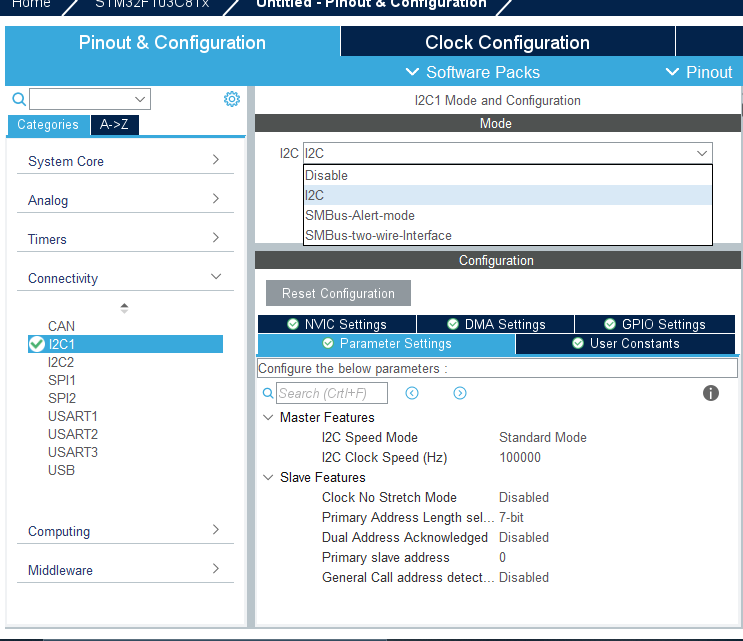
\includegraphics[width=.8\textwidth]{figure/4_7.png}
     \caption{I2C Configuration in STMCube}
     \label{fig:i2c-config}
 \end{figure}
 
 \subsubsection{I2C Functions}

For the available functions provided by the HAL that are needed in the project:

\begin{enumerate}
    \item \textbf{MX\textunderscore I2Cx\textunderscore Init()}: written by default in the main to initialize the intended I2C
where the x is replaced by the number of the used I2C.
    \item \textbf{HAL\textunderscore I2C\textunderscore Mem\textunderscore Write()}: This function is used to write the data on the I2C bus to send it to the connected slaves.
    \item \textbf{HAL\textunderscore I2C\textunderscore Mem\textunderscore Read()}: This function is used to read the data on the I2C bus that is sent by some slave.
\end{enumerate}
\chapter{V2V Vehicle Implementation}

\section{Inertia Measurement Unit (IMU)}
\subsection{The data collected and the used sensor}
There are many scenarios for a moving car; starting the engine and going from still to a certain speed, stopping suddenly when the traffic sign becomes red, speeding up when going on highway, … etc. In these scenarios, the common thing is the changing of the speed due to acceleration. So, it was necessary to sense and collect the acceleration information.
To get the acceleration information, an MPU6050  IC is used. It contains a 3-axis gyroscope and a 3-axis accelerometer. So, the data collected from this IC is the acceleration from the 3-axis accelerometer, and the angular speed from the 3-axis gyroscope. The accelerometer is made using MEMS technology. The direction of the acceleration and angular speed for every axis is shown in figure \ref{fig:orientation} .
\begin{figure}[h]
    \centering
    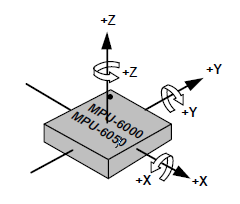
\includegraphics{figure/5-1.png}
    \caption{Orientation of Axes of Sensitivity and Polarity of Rotation}
    \label{fig:orientation}
\end{figure}
\clearpage
To use this IC, the module GY-521 MPU6050 is used. The module is shown in figure \ref{fig:mpu6050}.

\begin{figure}[h]
    \centering
    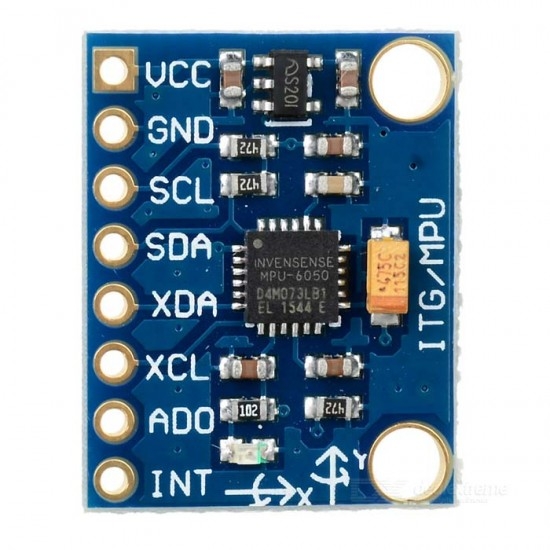
\includegraphics[scale=.5]{figure/5-2.jpeg}
    \caption{GY-521 MPU6050}
    \label{fig:mpu6050}
\end{figure}

The features of this module are as following below:
\begin{itemize}
    \item Power supply: 3-5V.
    \item Communication modes: standard I2C communications protocol.
    \item Chip built-in 16bit AD converter, 16-bit data output.
    \item Tri-Axis angular rate sensor (gyroscope) with a sensitivity up to 131 LSBs/dps and a full-scale range of ±250, ±500, ±1000, and ±2000dps.
    \item Tri-Axis accelerometer with a programmable full-scale range of ±2g, ±4g, ±8g and ±16g.
\end{itemize}

Although this module has both accelerometer and gyroscope, but the focus would be on the acceleration and not the angular speed.
Theoretically, the orientation of the car and its heading can be calculated from the angular speed by integrating the angular speed of the Z-axis as the equation below.
\[ \omega = \frac{d \theta}{dt}\]
\[ \theta = \int_{}^{} \omega \,dx \]

But this is not applicable at hardware level, due to the existence of noise. By adding noise to the system, the equation becomes as following below.
\[ \theta = \int_{}^{} \omega \,dx + \int_{}^{} N \,dt \]
\[ \theta = \theta_{theoretical} + \int_{}^{} N \,dt \]
The noise is integrated with respect to time. So, it  is accumulating with time. That makes the value read from the gyroscope in constant increasing due to noise and not reliable.
To solve this problem, a compass is needed to detect the orientation of the car. This would be discussed later in this chapter.

\subsection{The configuration of the sensor}
\subsubsection{Configuring the I2C address}
As discussed earlier, the GY-521 MPU6050 module uses the I2C communication protocol to communicate with the microcontroller. The I2C communication protocol depends on the addresses of the master and the slave to be able to communicate with each other. So, the address of this module should be known to the microcontroller to be able to communicate with it.
This module can have two different addresses, this is helpful if it was needed to work with two of these modules. So, every module has a different address, and the microcontroller can communicate with each one separately. The address of the module is set using the pin AD0. The next table shows the address of this module in different states of the pin AD0.
\begin{table}[h]
\def\arraystretch{1.5}
\centering
\begin{tabular}{| c | c |}
\hline
 \textbf{AD0 State} &  \textbf{I2C Address} \\
 \hline
 Low &  $(1101000)_2$ \\
 \hline
 High & $(1101001)_2$ \\
 \hline
\end{tabular}
\end{table}

The user chooses the address by hardware, using the AD0 pin, and configure it in the code.
\clearpage
\subsubsection{Configuring the accelerometer scale}
This module also has a programmable full-scale range. It can be four different ranges as discussed earlier. But there is trade off between the range and the resolution of the accelerometer. As the range increases, the resolution increases. The next table shows the relation between the scale and the resolution of this module. The gravity is assumed to be 10 m/s2.

\begin{table}[h]
\def\arraystretch{1.5}
\centering
\begin{tabular}{| c | c |}
\hline
 \textbf{Scale (m/$s^2$)} &  \textbf{Resolution (m/$s^2$)} \\
 \hline
 -20 : +20 &  $610 * 10 ^ -6$ \\
 \hline
 -40 : +40 & $1.22 * 10 ^ -3$ \\
 \hline
  -80 : +80 & $2.44 * 10 ^ -3$ \\
 \hline
  -160 : +160 & $4.88 * 10 ^ -3$ \\
 \hline
 
\end{tabular}
\end{table}
The user configure the range in the code.
\subsubsection{Configuring the order of the LPF}
This module has an internal digital low pass filter (DLPF) to reduce the noise. The user can configure the order of this filter. The higher the order of the DLPF, the smaller the bandwidth, thus the lower the noise effect. But there is tradeoff between the bandwidth of the DLPF and the delay. The higher the order of DLPF, the higher the delay. The next table shows the relation between the delay and the order of the DLPF.

\begin{table}[h]
\def\arraystretch{1.5}
\centering
\begin{tabular}{| c | c | c |}
\hline
 \textbf{DLPF Order} &  \textbf{Bandwidth (Hz)
}  & \textbf{Delay (ms)}\\
 \hline
 0 &  260 & 0 \\
 \hline
1 &  184 & 2.0 \\
 \hline
 2 &  94 & 3.0 \\
 \hline
3 &  44 & 4.9 \\
 \hline
4 &  21 & 8.5 \\
 \hline
 5 &  10 & 13.8 \\
 \hline
 6 &  5 & 19.0 \\
 \hline

\end{tabular}
\end{table}

The user configures the order of DLPF in the code.
\clearpage
\subsubsection{Configuring the sample rate}
The sample rate of this module is following the next formula

\[sample \! rate = \frac{Gyroscope Output Rate}{Prescaler + 1} \]
The gyroscope output rate is 8 kHz when the DLPF is disabled and 1 kHz otherwise.
The user can configure the sample rate using the prescaler value. The prescaler is an unsigned 8-bit number, so it varies from 0 to 255.
The user configures the sample rate in the code.

All the previous configurations that the user could change in the code is done in the file “imu\_config.h” where the configuration is done easily as shown in the code below.

\begin{lstlisting}

#ifndef	__IMU_CONFIG_H__
#define	__IMU_CONFIG_H__
/*	Defining the state of the pin AD0 of the IMU. */
#define	IMU_AD0_STATE					IMU_AD0_SET
/*	Defining the scale of the gyroscope. */
#define IMU_GYRO_SCALE					IMU_GYRO_SCALE_1000
/*	Defining the scale of the accelerometer. */
#define IMU_ACCEL_SCALE					IMU_ACCEL_SCALE_4G
/*	Defining the digital low pass filter(DLPF) order. */
#define	IMU_DLPF_ORDER					0x05UL
/*	Defining the state of the pin AD0 of the IMU. */
#define	IMU_SAMPLE_RATE_PRESCALER		0x00UL
#endif

\end{lstlisting}

\subsection{The functions of this sensor driver}
There are three main functions to be used by the user.
\begin{enumerate}
    \item \textbf{void HAL\_IMU\_Init(I2C\_HandleTypeDef *I2Cx)
    \item \textbf{void} HAL\_IMU\_Read\_Accel(I2C\_HandleTypeDef *I2Cx, IMU\_TypeDef *DataStruct)}
    \item \textbf{HAL\_StatusTypeDef HAL\_IMU\_Test(I2C\_HandleTypeDef *I2Cx)}
\end{enumerate}
\clearpage
These functions are used in the main as the user wants to its application.
\begin{enumerate}
    \item \textbf{void HAL\_IMU\_Init(I2C\_HandleTypeDef *I2Cx)}
    \begin{figure}[h]
        \centering
        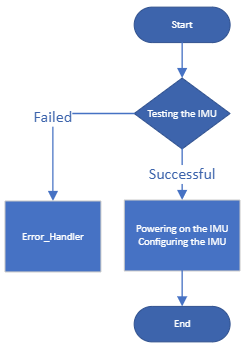
\includegraphics{figure/5-3.png}
        \caption{Flow chart of the initiation function}
    \end{figure}
    \begin{itemize}
    \item This function takes the I2C peripheral used to communicate with the IMU as input.
    \item This function does not return.
    \item It starts by testing the IMU using the function \textbf{HAL\_IMU\_TEST} which would be discussed later.
    \item If the test went successful, the program continues. But if it failed, the program calls the function \textbf{Error\_Handler} which is configurable by the user.
    \item The IMU is powered on and configured, as the user choose in “imu\_config.h” file, by writing specific values into its registers.
    \end{itemize}
    \item \textbf{void HAL\_IMU\_Read\_Accel(I2C\_HandleTypeDef *I2Cx, IMU\_TypeDef *DataStruct)}
    \begin{figure}[h]
    \centering
    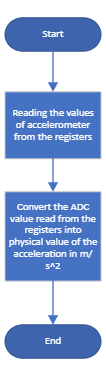
\includegraphics{figure/5-4.png}
    \caption{Flow chart of the reading function}
\end{figure}
    \begin{itemize}
        \item This function takes the I2C peripheral used to communicate with the IMU and pointer to the data struct containing the variables to store the accelerations as inputs.
        \item This function does not return.
        \item It starts by reading the values of the accelerations for the three axes in the registers of the MPU6050.
        \item These values are signed 16-bit value representing the acceleration of the car in the three axes.
        \item These values are then converted into a number representing the acceleration in $m/s^2$ and saved in the corresponding variables in the data struct.
        \item These conversions depend on the scale configured for the MPU6050.
        \item The conversion is done using the following formula
        \[ a = (16 - bit value) * (Resolution)\]
    \end{itemize}
    \item \textbf{HAL\_StatusTypeDef HAL\_IMU\_Test(I2C\_HandleTypeDef *I2Cx)}
    
    
    \begin{itemize}
        \item This function takes the I2C peripheral used to communicate with the IMU as input.
        \item This function returns the status of the test.
        \item There is a register in the module called WHO\_AM\_I register, this register is read only register with a fixed value equal to 0x68 in hexadecimal format.
        \item The test reads the value of this register and compare it to the value 0x68. If it is equal to this value, then the test is successful and it returns HAL\_OK. But if it was something else, the MPU6050 is reset by software and  it tries again to read the register for a certain number of tries.
        \item If the number of tries have exceeded the allowed number of tries, the function returns HAL\_ERROR.
    \end{itemize}
    \begin{figure}[h]
    \centering
    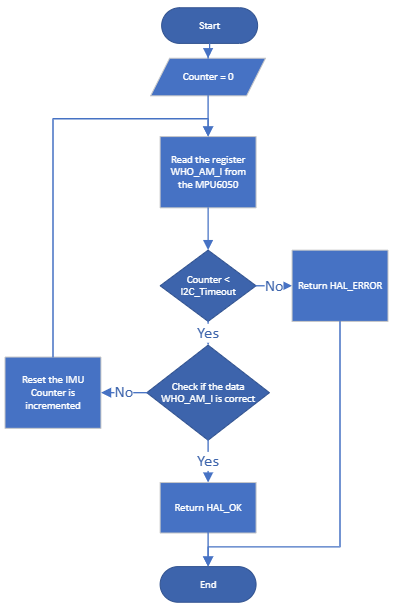
\includegraphics{figure/5-5.png}
    \caption{Flow chart of the testing function}
    \end{figure}
\end{enumerate}
\clearpage
\subsection{Testing the sensor}
To evaluate the sensor and its output values, the gravity is used.
We position the module in three different positions and read the values of acceleration from the three different axes.
\textit{The next table shows the three different positions.}


\begin{figure}[h]
    \centering
    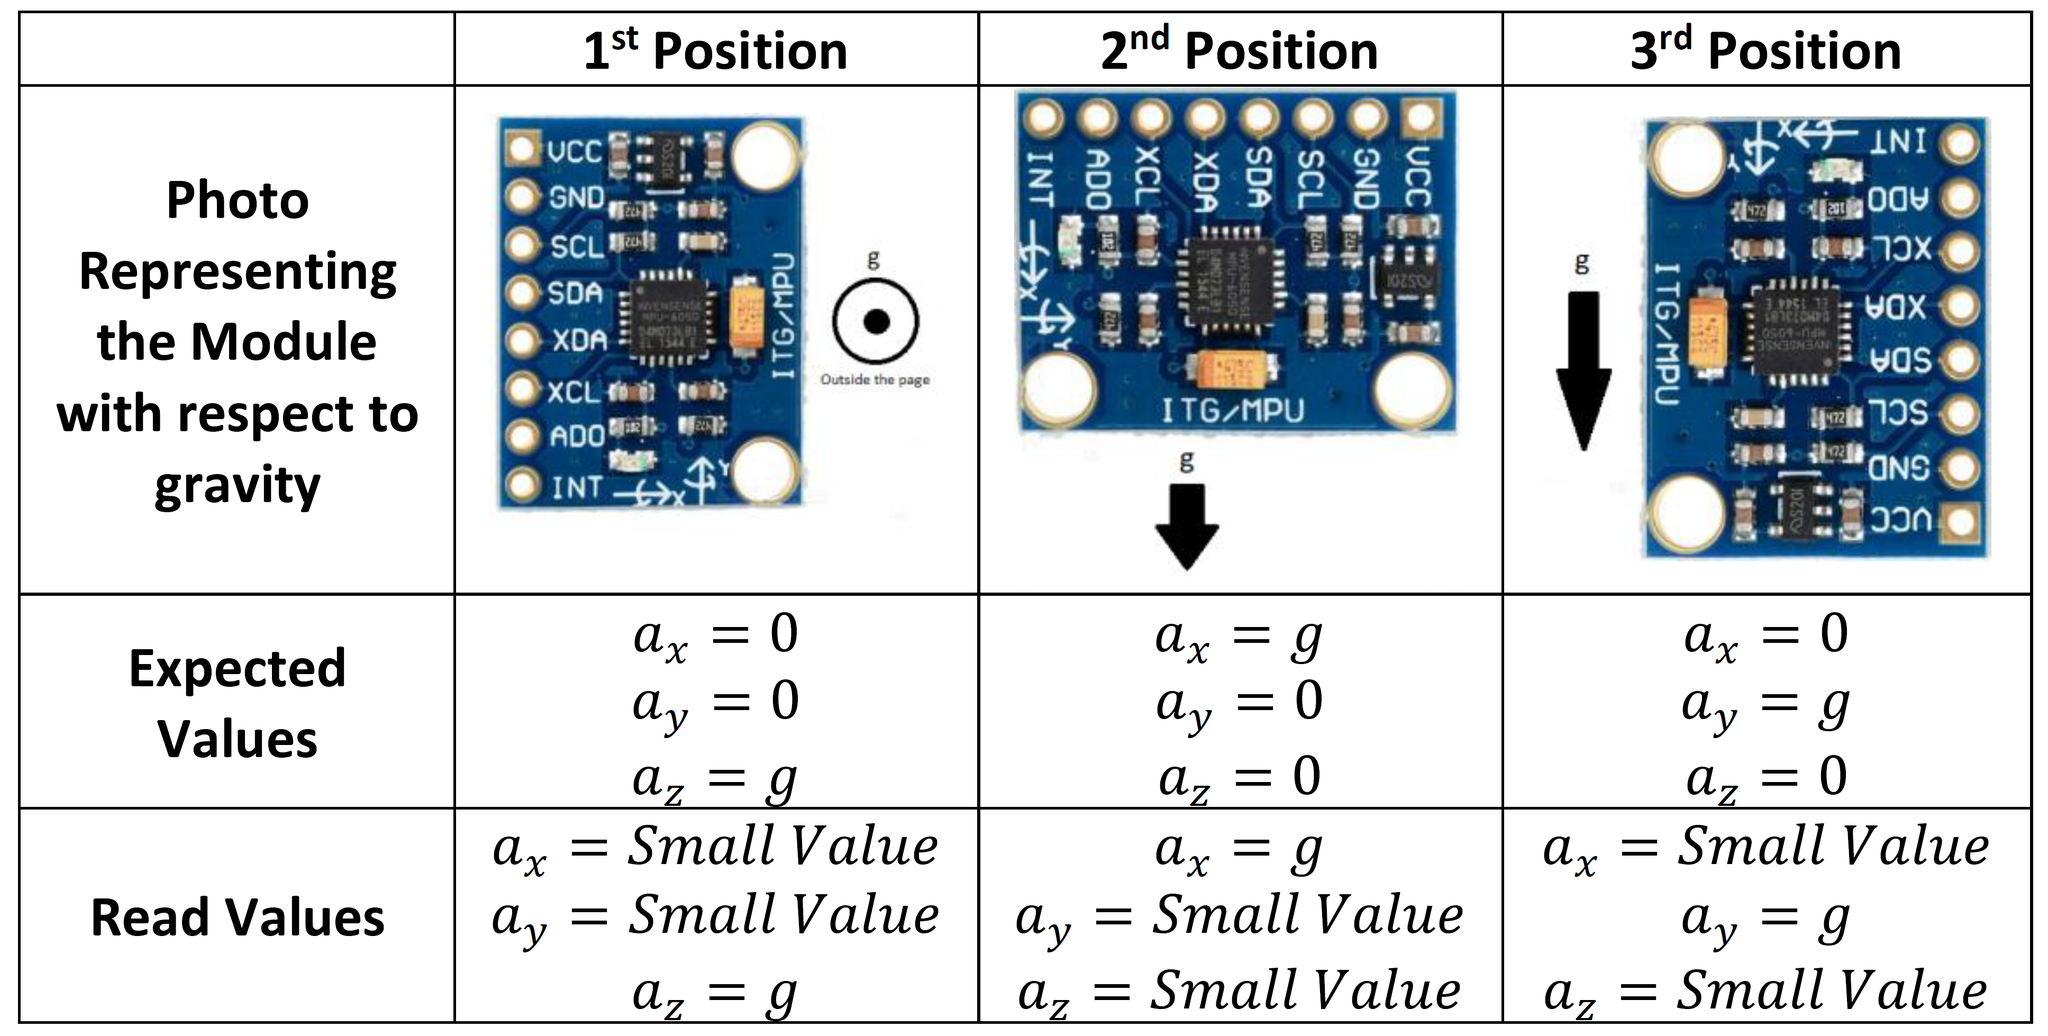
\includegraphics[scale=.2]{figure/5-6.png}
    \caption{IMU in three different positions}
\end{figure}
This means that the test went successful, and the IMU is working fine.

\section{Speed Measurement Unit}

\subsection{The data collected and the used sensor}
The main variable to be monitored in modern cars as well as ancient cars is the speed. Any car must have a speed monitoring system in it whether it is an analog system such as a pointer on scale or a digital system such as a lcd displaying the speed. This shows how important is the speed information for the vehicle.
There were two options for selecting the sensor used for the sensing the speed information.
\begin{figure}[h]
    \centering
    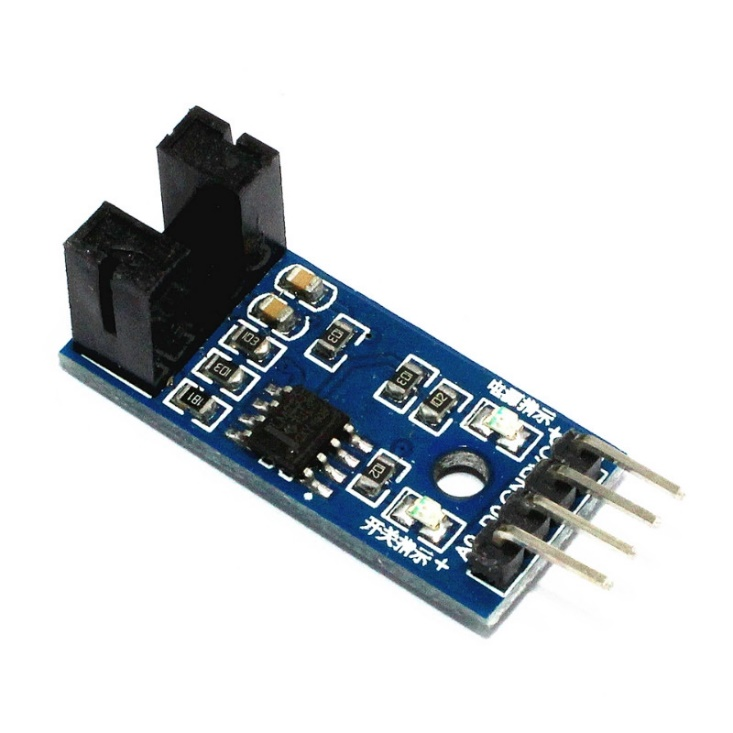
\includegraphics[scale=.5]{figuresEncoder/1.jpeg}
    \caption{IR Encoder}
\end{figure}
\begin{figure}[h]
    \centering
    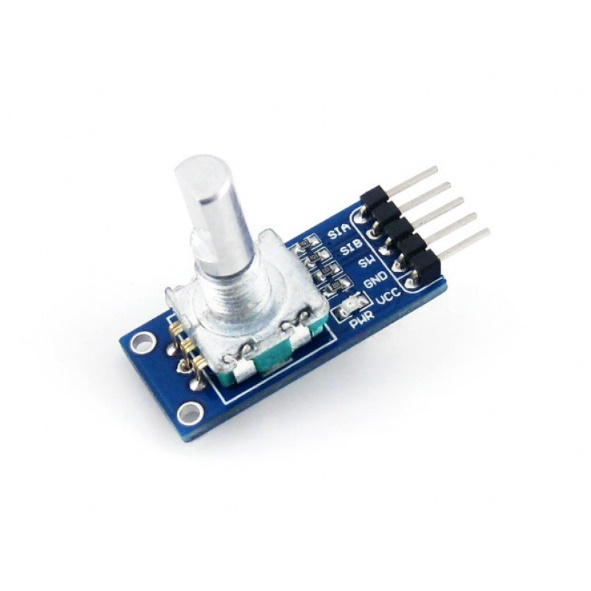
\includegraphics{figuresEncoder/2.jpeg}
    \caption{Shaft Rotary Encoder}
\end{figure}

The first option was the shaft rotary encoder. 
The working principle of this sensor is that there are two metal contacts separated apart from each other, and the common pin is a gear. So, when the tooth of the gear touches the metal it the output is high, otherwise the output is low. So, when the shaft moves, a square pulse is generated on the two outputs, and since the two metals are separated apart, the two square waves are phase shifted.

\begin{figure}[h]
    \centering
    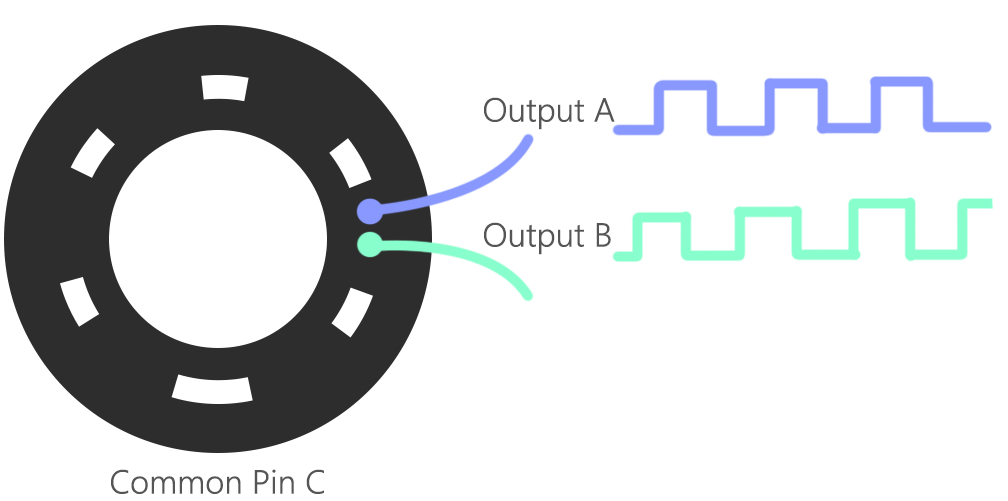
\includegraphics[scale=.4]{figuresEncoder/3.png}
    \caption{The working principle of shaft rotary encoder}
\end{figure}

 The advantages of the shaft rotary encoder
\begin{enumerate}
    \item Its simple system.
    \item It can detect the direction of the rotation whether it is clockwise (CW) or counterclockwise (CCW). This is done using the phase shift information between the two square pulses.
    \item It is compatible with the micro controller using the encoder mode in the timer peripheral.
\end{enumerate}

The disadvantages of the shaft rotary encoder
\begin{enumerate}
    \item There is bouncing because the system is mechanical switch. This problem can be solved using digital low pass filter (DLPF) in the timer peripheral in the encoder mode.
    
    \item It is connected directly to the motor which is seen as a load and can effect the speed of the motor specially if the shaft of the sensor is stuck.
    
\end{enumerate}
The second option was the infra-red (IR) encoder .
The working principle of this sensor is that there is an IR LED is a side, an IR detector in the other side, and a comparator. When the beam is continuous from the LED to the receiver, the output from the module is high. When the beam is blocked and was not received by the IR detector, the output from the module is low.

\begin{figure}[h]
    \centering
    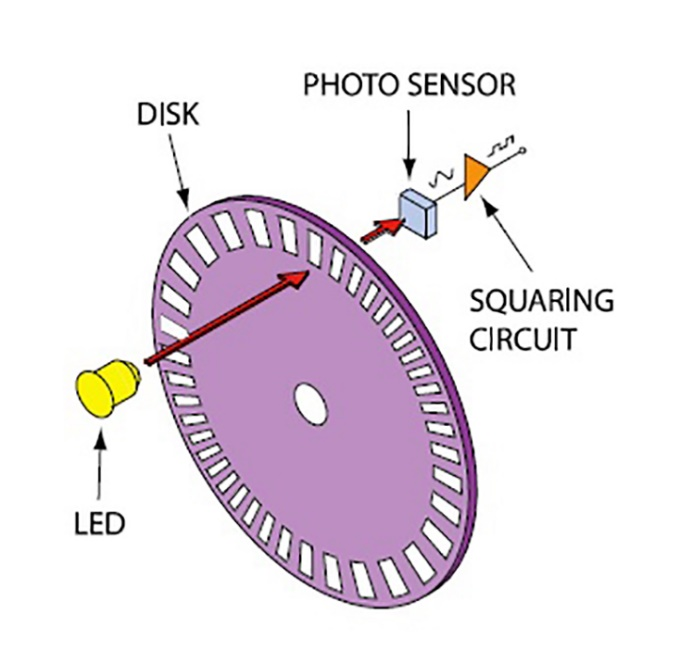
\includegraphics[scale=.7]{figuresEncoder/4.jpeg}
    \caption{The working principle of the IR encoder}
\end{figure}

The advantages of the IR encoder
\begin{itemize}
    \item There is no physical contact between the sensor and the motor. So, there is no load on the motor.
    \item It is very fast and reliable.
    \item The square wave output is perfect and has no bouncing.
\end{itemize}

The disadvantages of the IR encoder
\begin{itemize}
    \item It can’t detect the direction of the rotation.
\end{itemize}
The sensor used in this project would be the IR encoder.

\subsection{The configuration of the sensor}
The  sensor is used to calculate the revolution per minute (RPM).
The calculation of the RPM is following the next formula
\[ RPM = \frac{No. of revolutions}{Time elapsed}\]

There are two timer peripherals used to calculate the RPM; one is used to act as counter to count the number of revolutions, the other is used to act as timer to act as stopwatch for the time elapsed.
To calculate the RPM in this project, the number of revolutions is sampled after a specific period the user configure it previously.

\clearpage
\subsubsection{Configuring the number of pulses in one revolution}

There is a wheel with slots in it is attached to the motor shaft and displaced between the IR LED and IR receiver, the number of slots in the wheel represents the number of pulses in one cycle.
\begin{figure}[h]
    \centering
    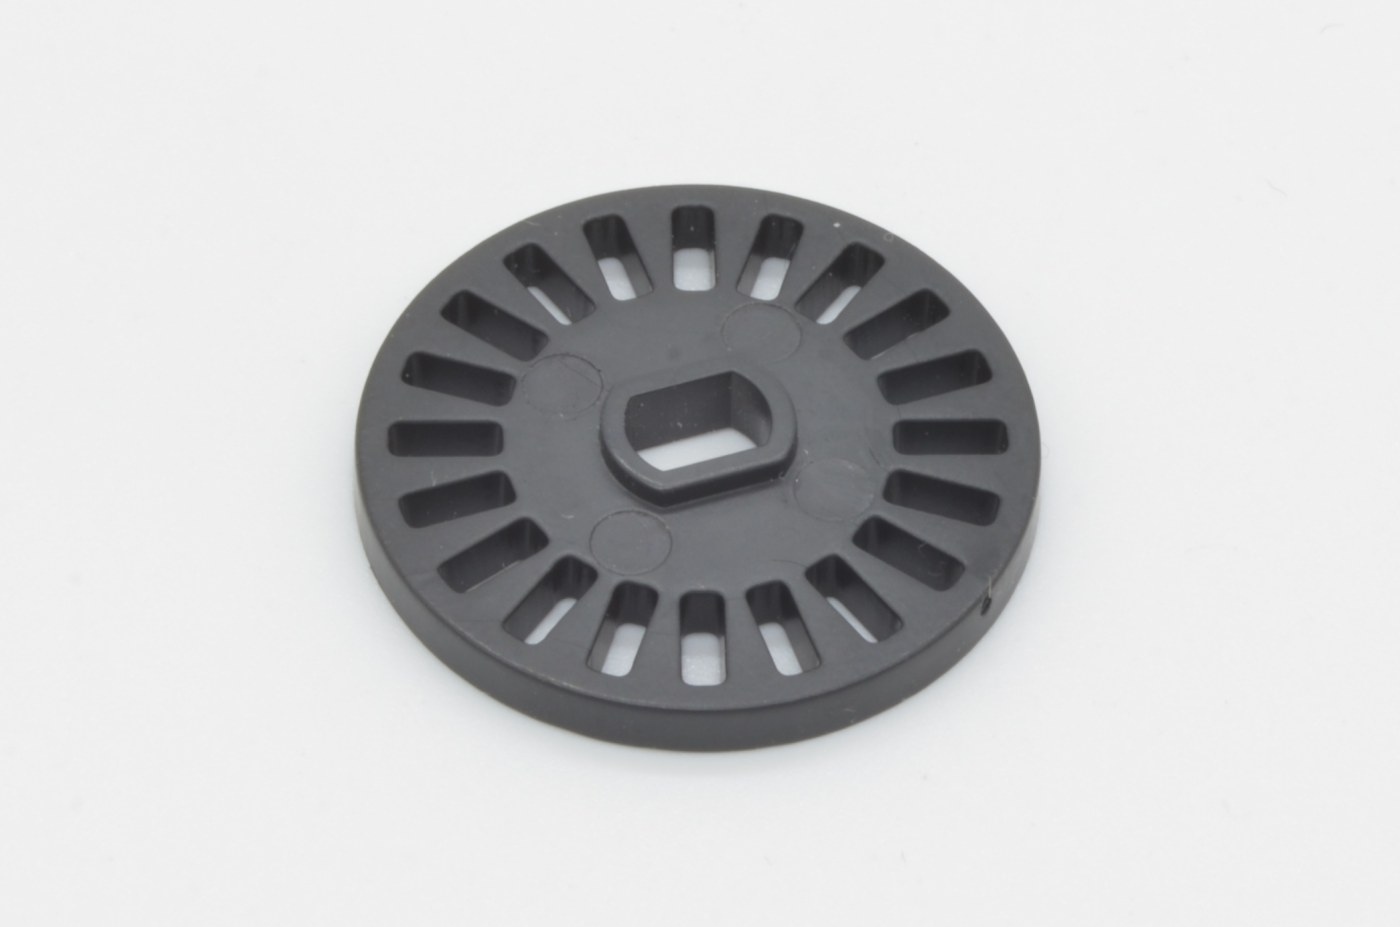
\includegraphics[scale=.2]{figuresEncoder/5.jpeg}
    \caption{The wheel connected to the shaft of the motor}
\end{figure}
The user configures this number in the code. In this project it is 20 slots.

\subsubsection{Configuring the counter}
To configure the counter, the clock source of the timer is chosen to be ETR2. This allows the timer peripheral to update with external clock.
Note that only timer 1 and timer 2 can be counter from the external source.
Also, the auto reload value must be enabled.
\begin{figure}[h]
    \centering
    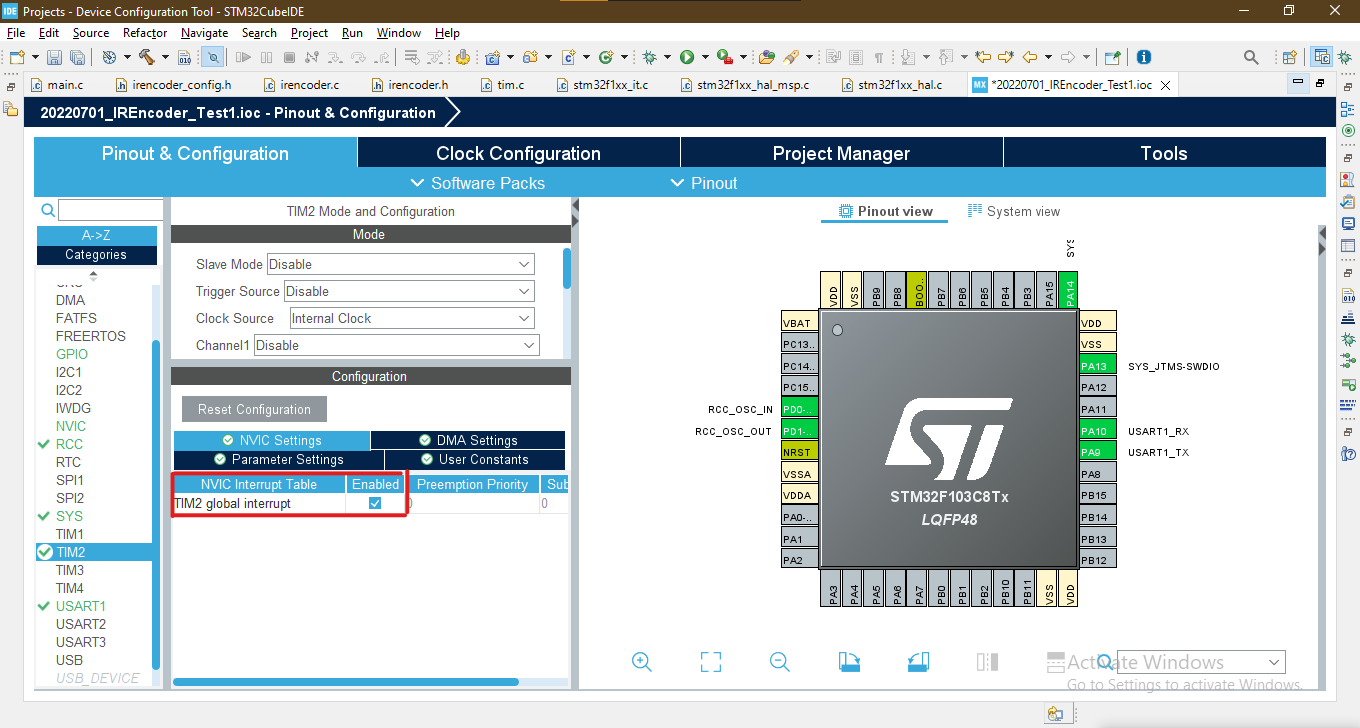
\includegraphics[scale=.4]{figuresEncoder/6.png}
    \caption{Configuring the counter in STM32CubeIDE}
\end{figure}
The user configures this in the STM32CubeIDE program.
\clearpage
\subsubsection{Configuring the timer}
To configure the timer, the clock source of the timer is chosen to be internal. This allows the timer peripheral to act as clock.
There are two internal clocks for the timers, as shown in the block diagram, from the datasheet, that timer 1 clock source is APB2, and the other timers are from APB1.

\begin{figure}[h]
    \centering
    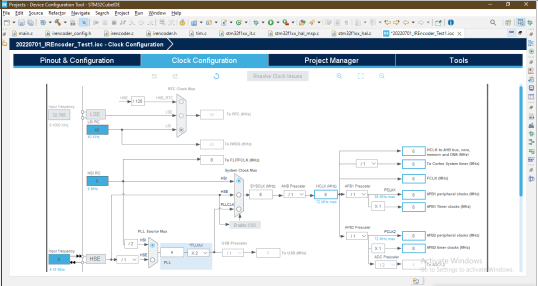
\includegraphics[scale=.8]{figuresEncoder/7.png}
    \caption{Clock Configuration in the STM32CudeIDE}
\end{figure}

\begin{itemize}
    \item The auto reload value must be enabled.
    \item The interrupt of this timer must be enabled.
\end{itemize}

\begin{figure}[h]
    \centering
    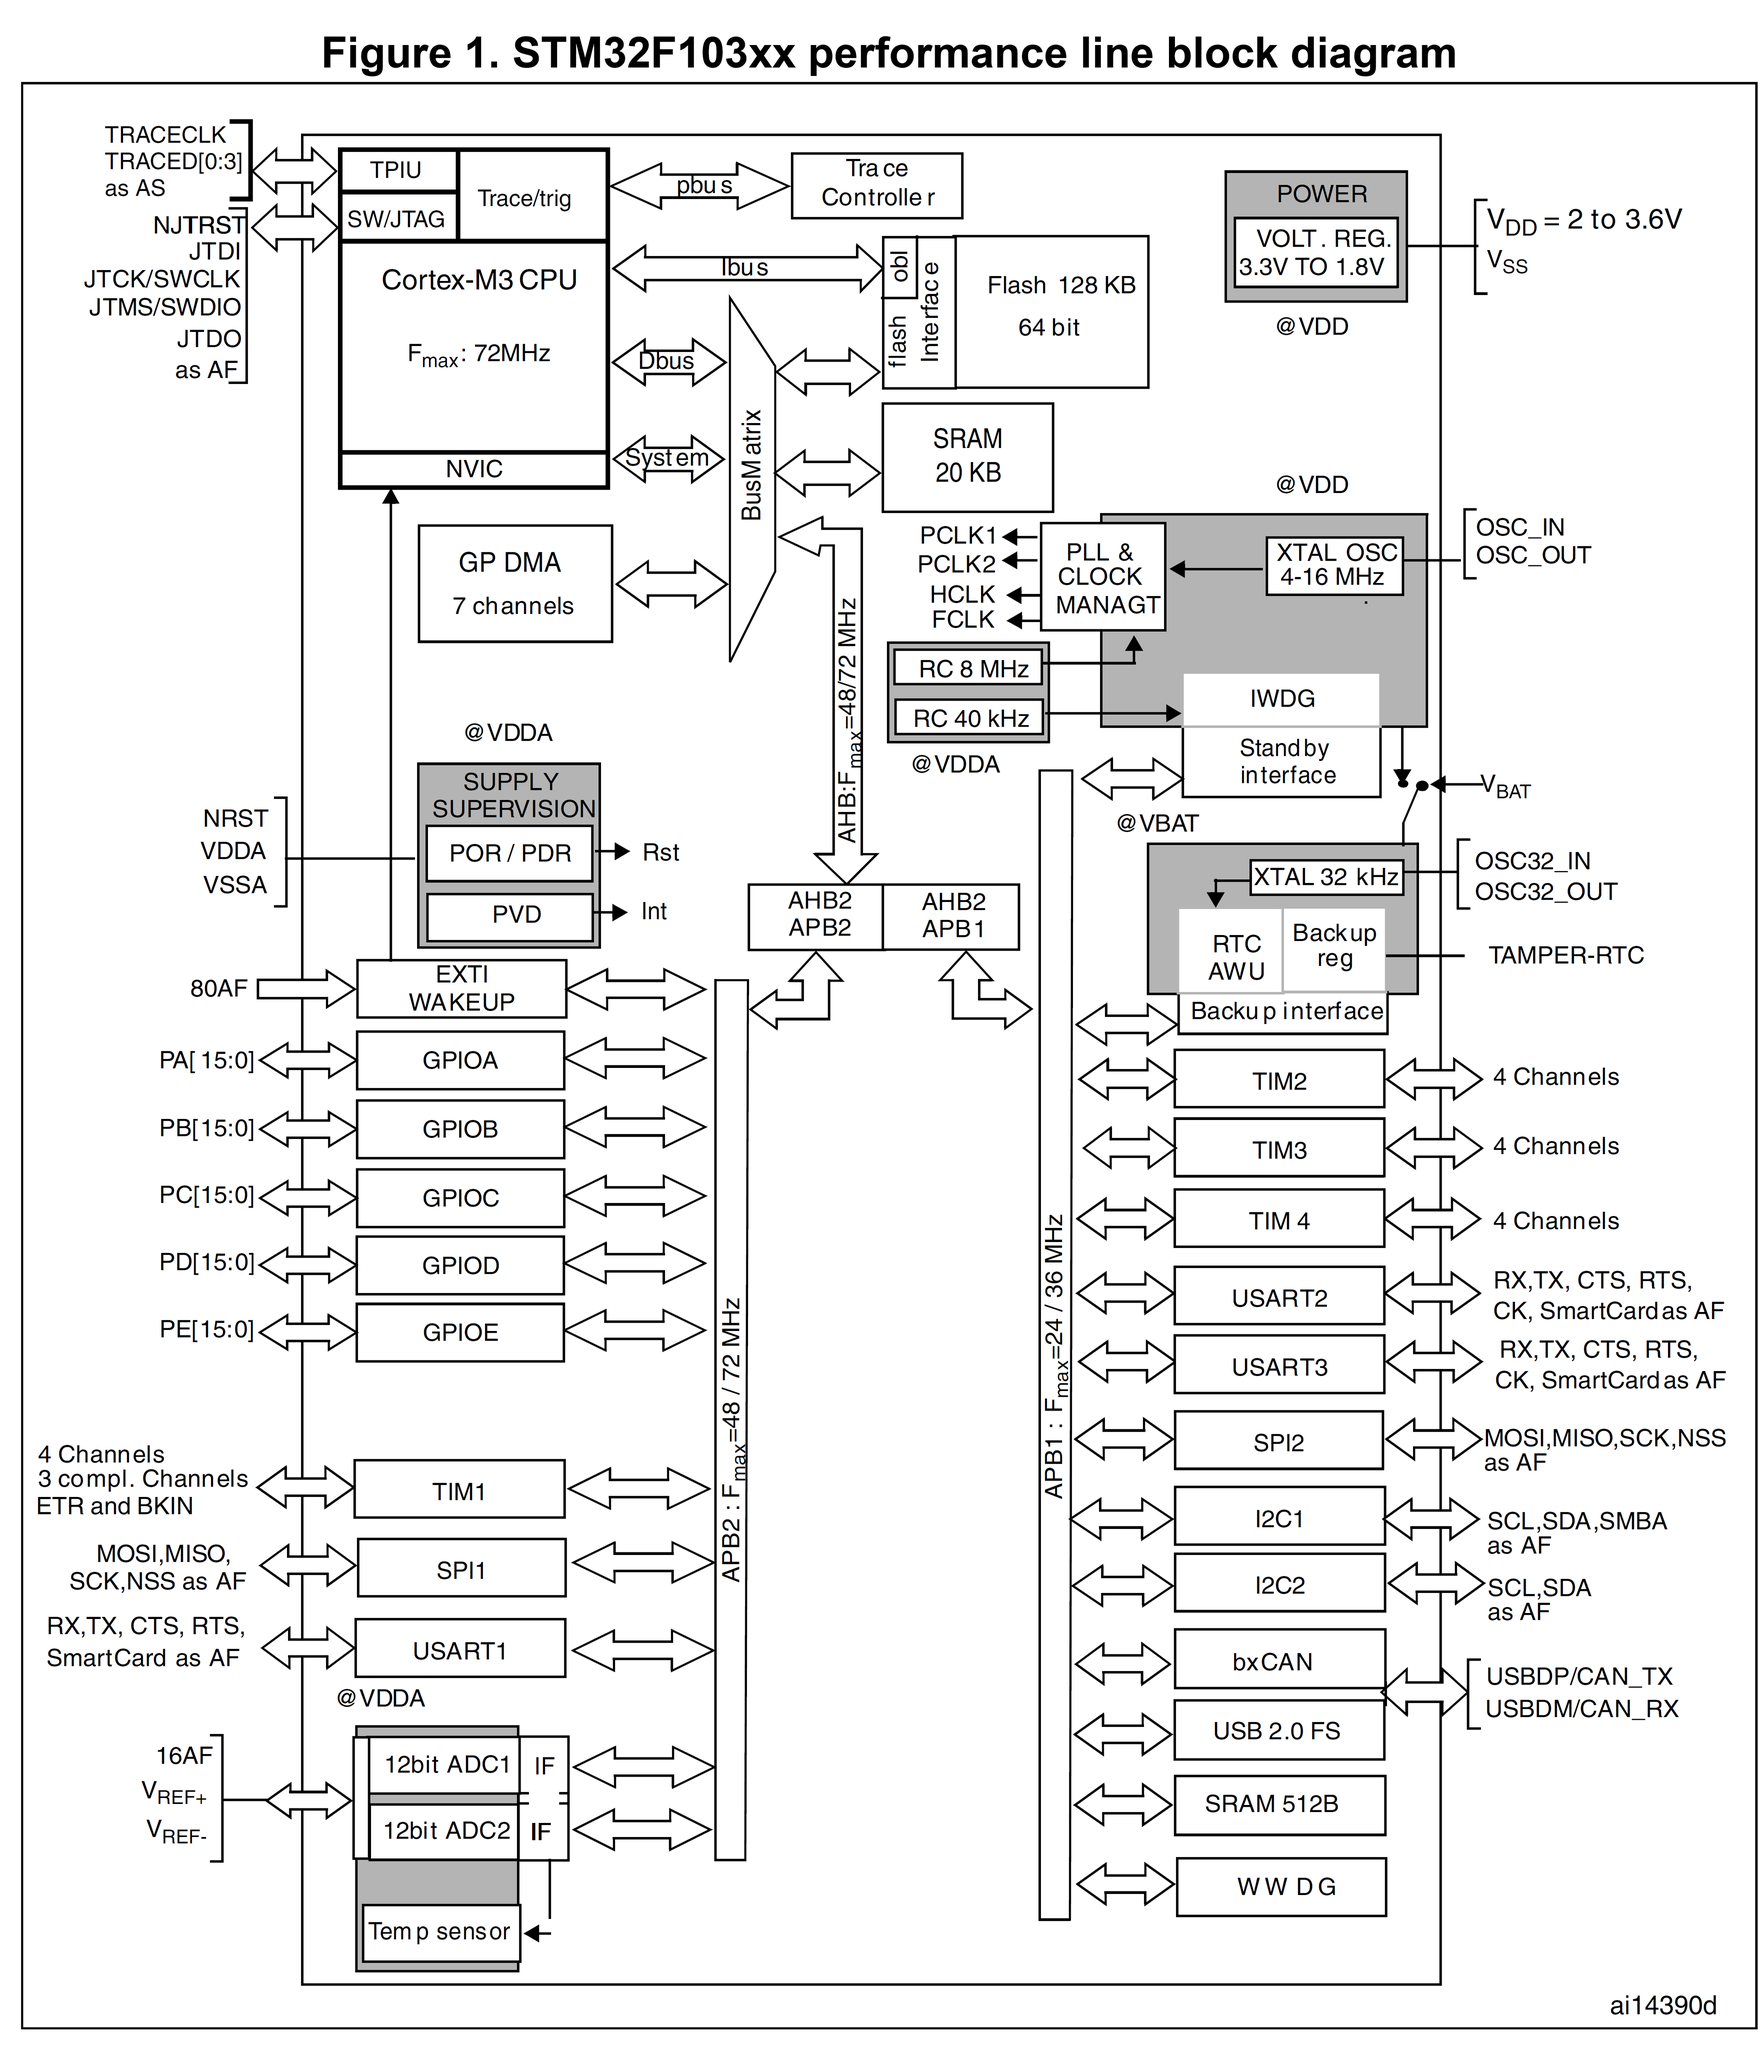
\includegraphics[scale=.22]{figuresEncoder/8.png}
    \caption{STM32F103C8T6 Block Diagram}
\end{figure}

\begin{figure}[h]
    \centering
    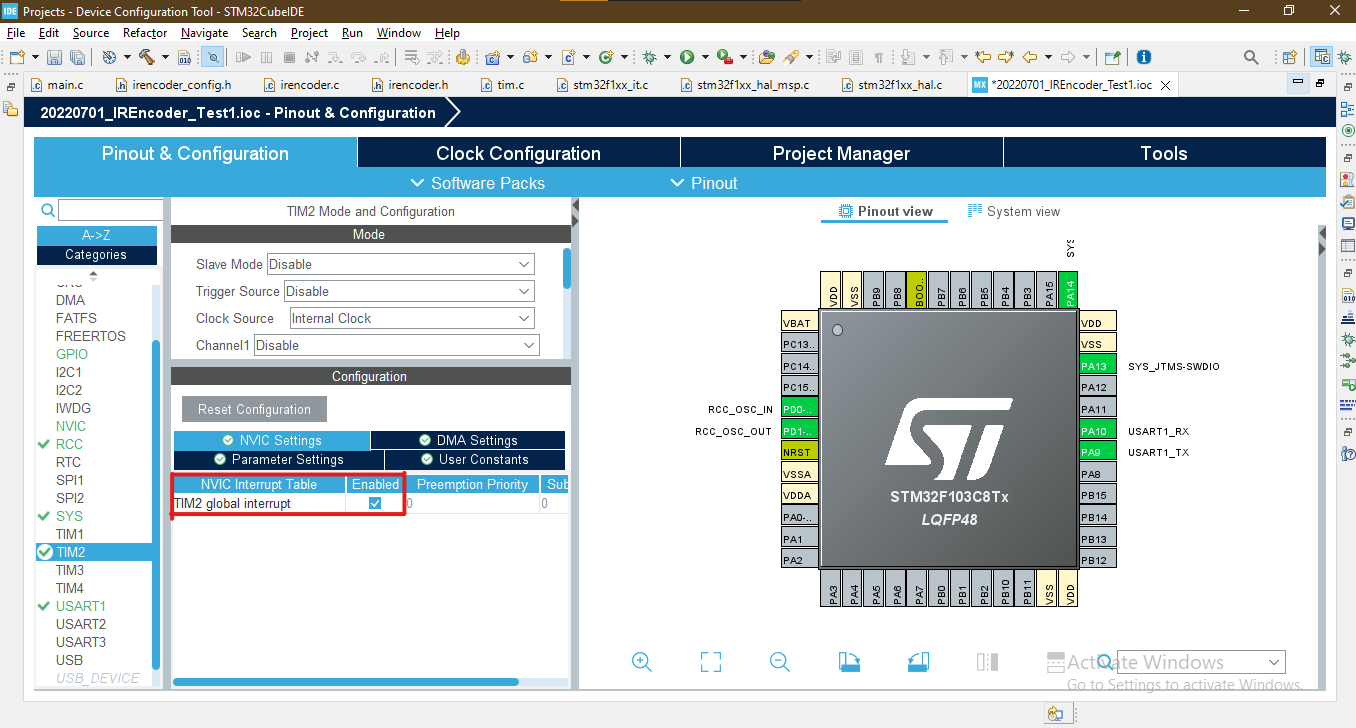
\includegraphics[scale=.34]{figuresEncoder/9.png}
    \caption{Configuring the timer in STM32CubeIDE (1)}
\end{figure}

\begin{figure}[h]
    \centering
    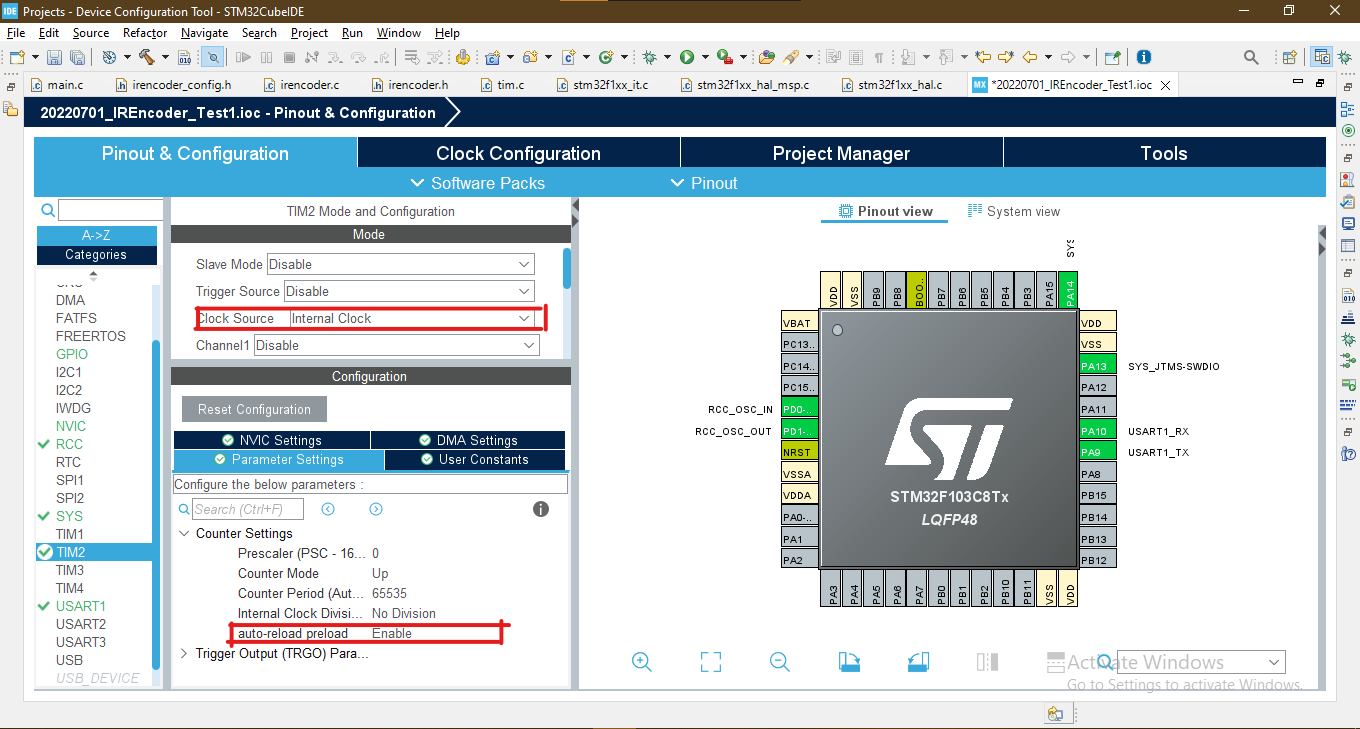
\includegraphics[scale=.33]{figuresEncoder/10.png}
    \caption{Configuring the timer in STM32CubeIDE (2)}
\end{figure}
\clearpage
\subsubsection{Configuring the timer clock}
Configuring the timer clock is done by the page of clock configuration in the STM32CudeIDE program as discussed earlier. But the additional thing to do is to configure the value of this clock in the code to help the program to calculate the RPM correctly. This configuration is done in the code.

\subsubsection{Configuring the period}
As discussed earlier, to calculate the RPM, the number of revolutions is sampled after a fixed period. This period is configured by the user.
This configuration is done in the code.
All the configurations that were done in the code, are modified in the file “irencoder\_config.h” easily.

\begin{lstlisting}
#ifndef __IRENCODER_CONFIG_H__
#define __IRENCODER_CONFIG_H__
/*	Defining the number of slots of the wheel attached to the motor. */
#define IRENCODER_ONE_CYCLE_PULSES		20
/*	Defining the clock frequency of the timer in kHz. */
#define IRENCODER_TIMER_CLK		8000
/*	Defining the method used to calculate the RPM. */
#define IRENCODER_RPM_CALCULATION		IRENCODER_RPM_FIXED_TIME
#endif

\end{lstlisting}

\section{The functions of this sensor driver}
\begin{enumerate}
    \item \textbf{void HAL\_IREncoder\_Start(TIM\_HandleTypeDef *Counter,\\TIM\_HandleTypeDef *Timer)}
    \item \textbf{void HAL\_IREncoder\_Stop(TIM\_HandleTypeDef *Counter, \\TIM\_HandleTypeDef *Timer)}
    \item \textbf{void HAL\_TIM\_PeriodElapsedCallback(TIM\_HandleTypeDef *htim)}
\end{enumerate}
These functions are used in the main depending on the user needs.
\clearpage
\begin{enumerate}
    \item \textbf{void HAL\_IREncoder\_Start(TIM\_HandleTypeDef *Counter,\\TIM\_HandleTypeDef *Timer)}
    \begin{figure}[h]
        \centering
        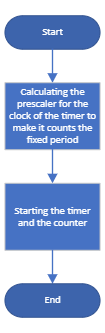
\includegraphics[scale=.6]{figuresEncoder/11.png}
        \caption{Flow Chart of the starting function}
    \end{figure}
    \begin{itemize}
        \item This function takes the timer and the counter as inputs.
        \item This function has no return.
        \item It first configures the timer so that it overflows after the fixed period defined by the user. That is the reason why the timer interrupt is activated. The calculation of the RPM is in the callback function of the timer interrupt.
        \item Starting both the timer and the counter. Notice that the timer is started in interrupt mode and the counter is started in the normal mode.
    \end{itemize}
    
     \item \textbf{void HAL\_IREncoder\_Stop(TIM\_HandleTypeDef *Counter, \\TIM\_HandleTypeDef *Timer)}
    \begin{itemize}
        \item This function takes the timer and the counter as inputs.
        \item This function has no return.
        \item This function has no return.
        \item It stops both the timer and the counter.
    \end{itemize}
    \clearpage
    \item \textbf{void HAL\_TIM\_PeriodElapsedCallback(TIM\_HandleTypeDef *htim)}
    \begin{figure}[h]
        \centering
        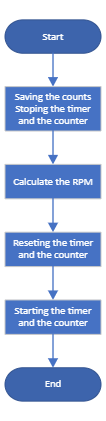
\includegraphics[scale=.6]{figuresEncoder/12.png}
        \caption{Flow Chart of the callback function}
    \end{figure}
    \begin{itemize}
        \item This function isn’t called by the user, but it starts when an interrupt occurs.
        \item It saves the value stored in the register of the counter as pulses.
        \item It stops the counter and the timer to prevent another interruption during the calculation.
        \item It calculates the RPM as the formula discussed earlier.
        \item It Resets the timer and the counter to be ready for the next iteration and parsing.
        \item The counter and the timer are started.
    \end{itemize}
    
\end{enumerate}
\subsection{Testing the sensor}
To test the sensor, a motor with a relatively known low speed is connected to the IR Encoder, and the RPM value is monitored.
For the test to be successful, the value of RPM from the code calculation should match the value of the RPM from the motor.

\section{Orientation Measurement Unit}
\subsection{The data collected and the used sensor}
The person in the driver seat uses the steering wheel to direct the vehicle into the direction he wants to go. When he wants to go from a lane to another, a signal light is used to inform the other cars in the lane of the sudden change. This shows how important is the heading and the orientation information of the car.
Although there is a gyroscope in this project, but it is discussed in the inertia measurement unit section the reasons why it cannot be used to get the orientation.
So, the sensor used for the orientation and heading information is HMC5883L IC.
This sensor has a 3-axis Magneto resistive which figure \ref{fig:hm5883l} shows the direction of the axes.

\begin{figure}[h]
    \centering
    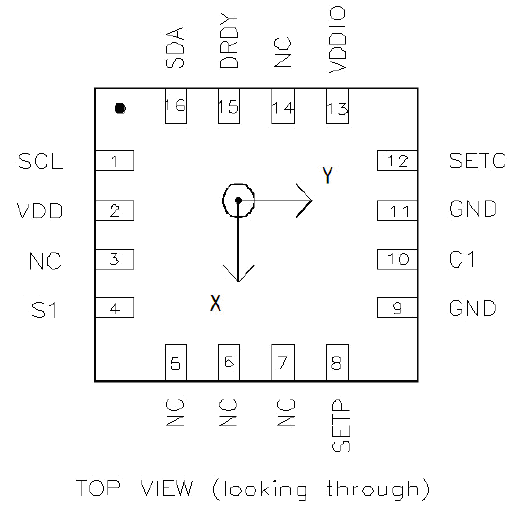
\includegraphics[scale=.6]{figures/1.png}
    \caption{The HMC5883L IC}
    \label{fig:hm5883l}
\end{figure}
\clearpage
The module used is GY-273 HMC5883L.
\begin{figure}[h]
    \centering
    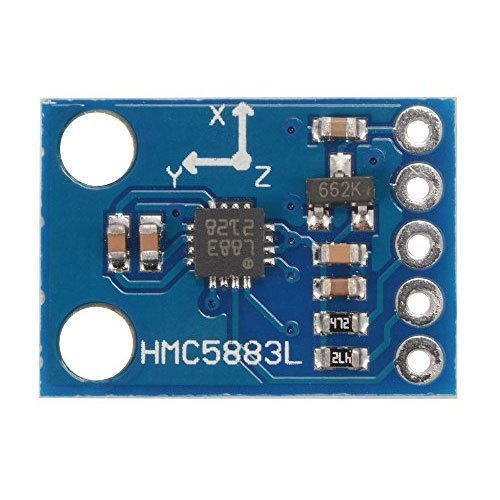
\includegraphics[scale=.5]{figures/2.jpeg}
    \caption{GY-273 HMC5883L Module}
\end{figure}
The main features of this module are as following below.
\begin{itemize}
    \item 3-Axis magneto resistive sensors.
    \item 12-bit analog digital converter.
    \item I2C digital interface.
\end{itemize}

This module is just a magneto sensor. So, it senses the magnetic field of the earth. Where the absolute value of the magnetic field sensed is maxed, it points to either north or south, where the magnetic field is strongest. If this value, the maximum value, is positive , then it points to north. And if this value, the maximum value, is negative, then it points to south.
\clearpage
\begin{figure}[h]
    \centering
    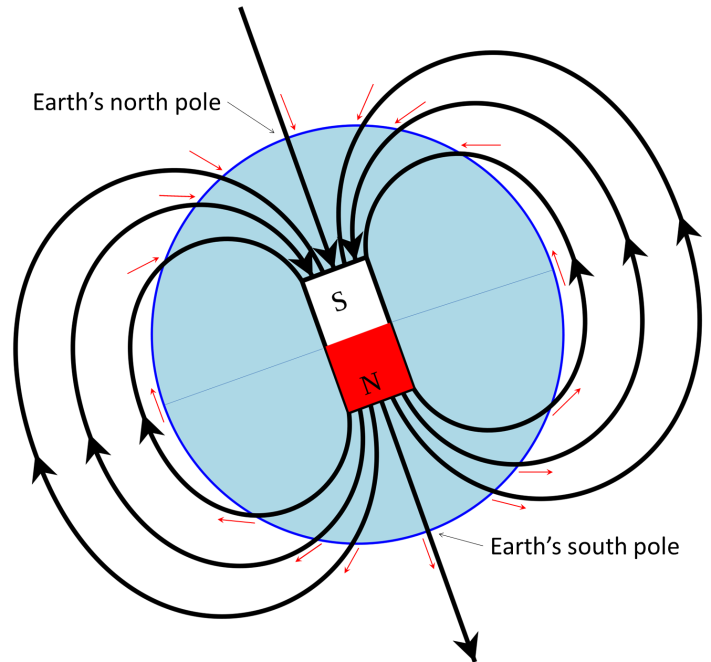
\includegraphics[scale=.3]{figures/3.png}
    \caption{Earth Magnetic Field}
\end{figure}
The working principle of this module is where the magneto sensor senses a positive max value in one of its axes, this axis points to the north. Knowing which direction is the north, the heading and the orientation is known with respect to the north as in maps.
Theoretically, the values sensed from the magneto sensors are moving on a circle its center is the origin point.
Since this module has x-axis and y-axis, this helps to find the directions effectively.
The existing of two axes, x-axis and y-axis, makes determining the angle between the x-axis and the north calculated using the following formula
\[ \theta = tan ^{-1} (\frac{magnetic value \in y-axis}{magnetic value \in x-axis})\]
There is 90 degrees shift between the two axes. So, if y-axis is used to determine the north with respect to itself, all that is needed to done is adding or removing 90 degrees to the output of the previous formula.

\subsection{The configuration of the sensor}
\subsubsection{Calibrating the sensor}
The sensor has a drift in the magneto sensor, that makes the center of the circle is not the origin point.
This can be shown by spinning the module 360 degrees while capturing the values of the magnetic field sensed in the registers of the module.
\clearpage
\begin{figure}[h]
    \centering
    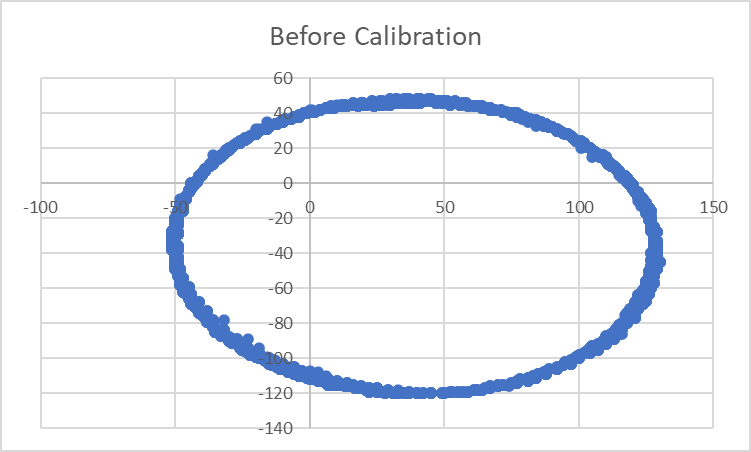
\includegraphics[scale=.3]{figures/4.png}
    \caption{The values of the magnetic fields before calibration}
\end{figure}
These values can be calibrated by calculating the offset of both axes.
The calculation would be following the next formula.

\[x_{new} = x_{dd} - \frac{x_{max} + x_{min}}{2} \]
\[y_{new} = y_{dd} - \frac{y_{max} + y_{min}}{2} \]

\begin{figure}[h]
    \centering
    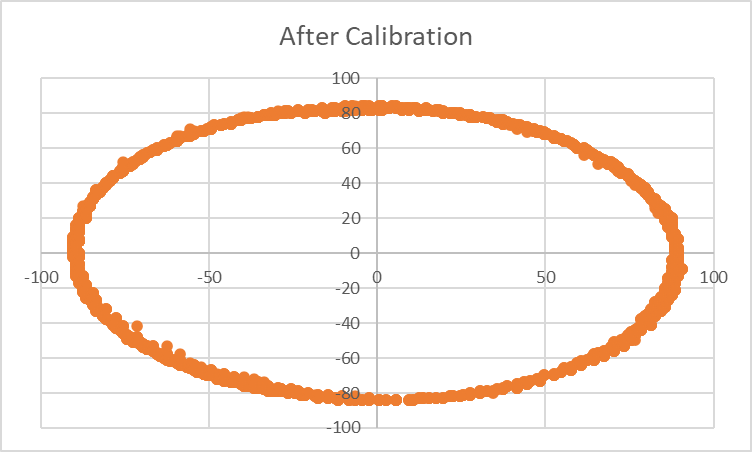
\includegraphics[scale=.3]{figures/5.png}
    \caption{The values of the magnetic fields after calibration}
\end{figure}
These calibrations are done by rotating the module 360 degrees to parse the values and calibrate the offset by code.

\subsubsection{Configuring the average sample rate}
The samples acquired from the magneto sensors can be averaged for more accuracy.
The average sample can be just one sample, two samples, 4 samples, or 8 samples.
The user configures this by the code.
\subsubsection{Configuring the output data rate}
The frequency of reading the value from the magneto sensors and storing into its registers is the data output rate.
The output rate could be one of the following values; 0.75, 1.5, 3, 7.5, 15, 30, or 75 Hz.
The user configures this by the code.
\subsubsection{Configuring the gain}
There are different ranges could be programmed by the user. But there is trade off between the range, or the gain, and the resolution. The higher the range the higher the resolution.
The next table shows the relation between the ranges available in this module and the resolution.

\begin{table}[h]
\def\arraystretch{1.5}
\centering
\begin{tabular}{| c | c |}
\hline
 \textbf{Range (Ga)} &  \textbf{Resolution (mGa/LSB)} \\
 \hline
 -0.88 to +0.88 &  0.73 \\
 \hline
 -1.3 to +1.3 & 0.92 \\
 \hline
 -1.9 to +1.9 & 1.22 \\
 \hline
  -2.5 to +2.5 & 1.52 \\
 \hline
   -4.0 to +4.0 & 2.27 \\
 \hline
   -4.7 to +4.7 & 2.56 \\
 \hline
   -5.6 to +5.6 & 3.03 \\
 \hline
   -8.1 to +8.1 & 4.35 \\
 \hline
 
\end{tabular}
\end{table}
This configuration can be done in the code.
\subsubsection{Configuring the I2C communication protocol}
The I2C can be in standard mode and fast mode.
In standard mode, the clock speed is 100 kHz. In fast mode, the clock speed is 100 kHz.
In fast mode, the clock speed is 400 kHz.
These configurations are done by the code.

All the configurations are modified in the file “compass\_config.h” easily.

\begin{lstlisting}
#ifndef __COMPASS_CONFIG_H__
#define __COMPASS_CONFIG_H__
/*	Defining the samples averaged per measurement output */
#define COMPASS_AVERAGE_SAMPLES		COMPASS_AVERAGE_SAMPLES_1
/*	Defining the data output rate */
#define COMPASS_DATA_OUTPUT_RATE	COMPASS_DATA_OUTPUT_RATE_15
/*	Defining compass gain value */
#define	COMPASS_GAIN				COMPASS_GAIN_1090
/*	Defining the mode of the I2C protocol *
#define COMPASS_I2C					COMPASS_I2C_STANDARD
#endif
\end{lstlisting}

\subsection{The functions of this sensor driver}
There are three functions.
\begin{enumerate}
    \item \textbf{void HAL\_Copmass\_Init(I2C\_HandleTypeDef *I2Cx)}
    \item \textbf{void HAL\_Compass\_Get(I2C\_HandleTypeDef *I2Cx, Compass\_TypeDef *DataStruct)}
    \item \textbf{HAL\_StatusTypeDef HAL\_Compass\_Test(I2C\_HandleTypeDef *I2Cx)}
\end{enumerate}

These three functions can be used by the user in the application.
\begin{enumerate}
    \item \textbf{void HAL\_Copmass\_Init(I2C\_HandleTypeDef *I2Cx)}
    \begin{figure}[h]
        \centering
        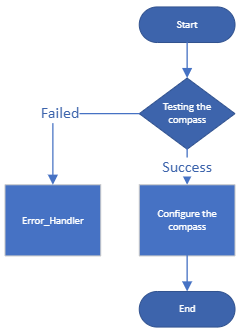
\includegraphics[scale=.6]{figures/6.png}
        \caption{Flow Chart of initiating function}
    \end{figure}
    \begin{itemize}
        \item This function takes the I2C peripheral used to communicate with the module as input.
        \item The function does not return.
        \item It starts by testing the compass using the function \textbf{HAL\_Compass\_Test}.
        \item if the test is successful, the code continues. If the test is failed, the function \textbf{Error\_Handler} is called. This function is configurable by the user.
        \item The configuration set by the user as discussed earlier would be set for the module.
    \end{itemize}
    
    
    \item \textbf{void HAL\_Compass\_Get(I2C\_HandleTypeDef *I2Cx, Compass\_TypeDef *DataStruct)}
    \begin{figure}[h]
        \centering
        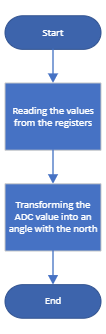
\includegraphics[scale=.8]{figures/7.png}
        \caption{Flow Chart of getting function}
    \end{figure}
    \begin{itemize}
        \item This function takes the I2C peripheral that communicate with module and a pointer to the data struct used to store the values of the angles as inputs.
        \item The function does not return.
        \item It starts by reading the values stored in the data registers of the sensor.
        \item It transforms these raw valued from the registers into an angle representing the angle between the axis and the north.
    \end{itemize}
    
    \clearpage
    \item \textbf{HAL\_StatusTypeDef HAL\_Compass\_Test(I2C\_HandleTypeDef *I2Cx)}
    \begin{figure}[h]
        \centering
        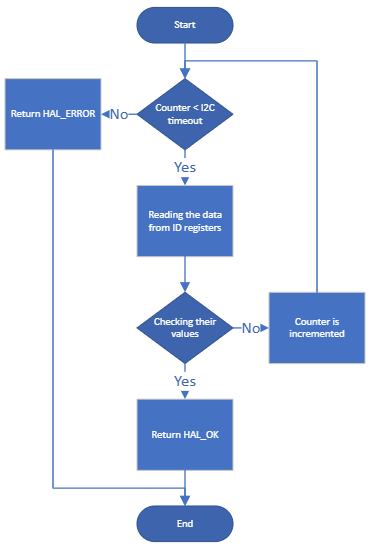
\includegraphics[scale=.6]{figures/8.png}
        \caption{Flow Chart of testing function}
    \end{figure}
    \begin{itemize}
        \item This function takes the I2C peripheral that communicates with the sensor as input.
        \item This function returns the status of the test.
        \item There are identification registers in the sensor, they are read only memory with fixed values.
        \item The function checks first the time out of the counter to see if the number of tries exceeded the allowed  number of iterations.
        \item Reading the value of the identification registers and comparing them with the default value of them.
        \item Returning HAL\_OK if the values are the same as the default values.
        \item Returning HAL\_ERROR if the values are not the same as the default and the number of tries exceeded the allowed number of iterations.
    \end{itemize}
\end{enumerate}
\subsection{Testing the sensor}
To test the sensor, its output is compared with values from external compass like the compass in most phones.
Theoretically, the two values should be the same.
When testing this sensor, the values from the sensor have offset by a value ranging from 1 degree to 7 degrees from the external compass.

\section{Location Measurement Unit}
Now, location for the vehicle needs to be measured, there were two options:
\begin{enumerate}
    \item GPS Data: It can be extracted from a GPS module, but as said before, the available modules need a very clear light of side to communicate with a satellite, so it was replaced with a Bluetooth module connecting with a mobile phone to get the GPS data from it since the mobile has a very accurate internal GPS.
    \newline The needed data from GPS was the longitude and latitude to determine exactly the vehicle position.
    \item Ultra sonic mechanism: Although GPS from mobile is more accurate than any single GPS module, it is has an error that may be affected on the calculations and analysis. Ultra sonic mechanism is very easy way to determine the distance between two device, it sends a chirp from the source, when it meets a surface, an echo reflected to the source. From the speed of echo and time it calculates the distance. This method is more accurate than GPS data.
\end{enumerate}

Despite of Ultra sonic accuracy, GPS data are extracted and used, it will help in some applications that will be discussed in chapter 9.

\subsection{Data collection from the module}
\begin{wrapfigure}{r}{5cm}
    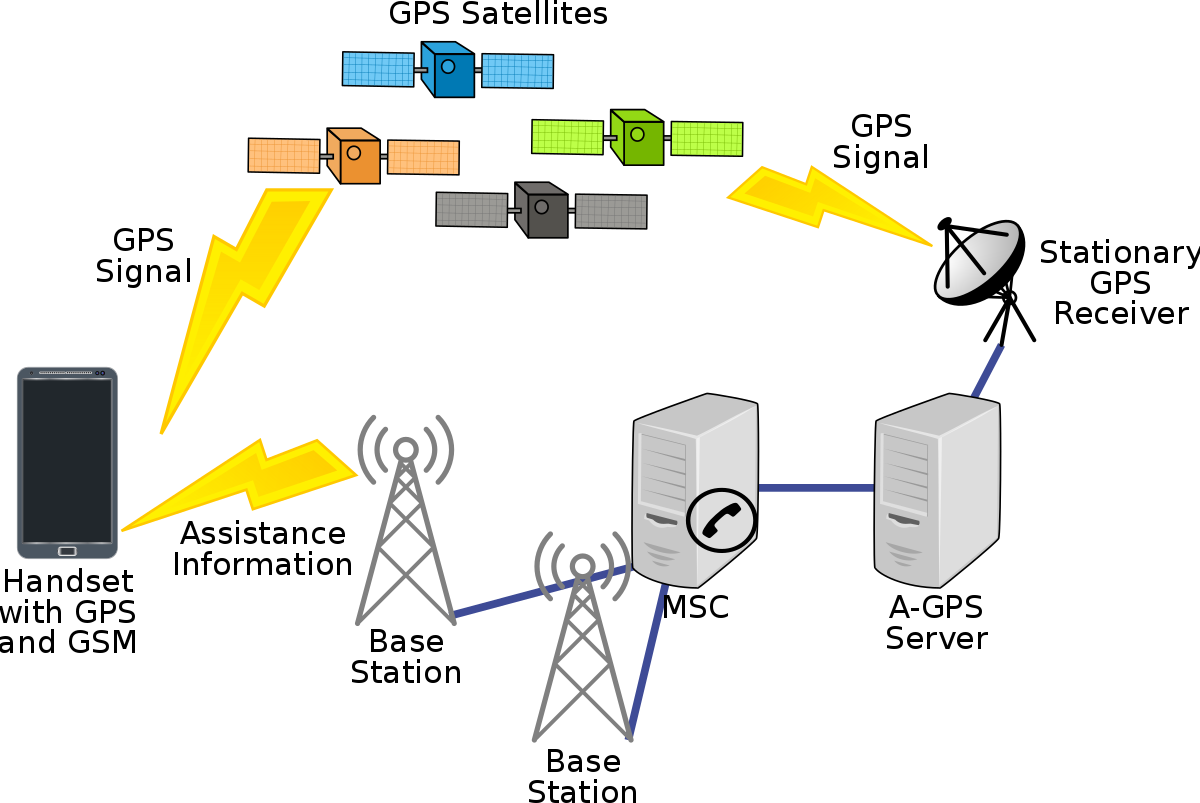
\includegraphics[width=0.5\textwidth]{figure/5_7.png}
    \caption{GPS block diagram in communication system}
    \label{fig:gps-block}
\end{wrapfigure}
The GPS module contains tiny processors and antennas that receive data sent from
the satellite through dedicated RF frequencies. From there, it’ll receive timestamps
from each visible satellite, along with other pieces of data. If the module’s antenna
can spot 4 or more satellites, it’s ability to accurately calculate its position and time,
which means this is the circuit that will allow us to know each car’s position
accurately.

\subsubsection{GPS Features}
\begin{itemize}
    \item Cold start time of 38 s and Hot start time of 1s.
    \item Supply voltage: 3.3 V.
    \item Configurable from 4800 Baud to 115200 Baud rates. (default 9600).
    \item SuperSense ® Indoor GPS: -162 dBm tracking sensitivity.
    \item 5Hz position update rate.
    \item Operating temperature range: -40 TO 85°C.
    \item UART TTL socket.
    \item EEprom to save configuration settings.
    \item Rechargeable battery for Backup.
    \item Separated 18X18mm GPS antenna.

\end{itemize}


\subsubsection{GPS working principle}
As shown in figure \ref{fig:gps-block}, there are three major segments in GNSS/GPS system:
\begin{enumerate}
    \item Space Segment (satellites)
    \begin{itemize}
        \item 24-32 MEO satellites.
        \item Obital period of 11 hr 55 min.
        \item 20,200 km Altitude above Earth.
        \item 5 to 8 satellites visible at all times from any
location any where in the world.
        \item These satellites have VERY accurate clocks on
board.
        \item The satellites continuously send radio signals
towards earth.
        \item These radio signals are picked up by GPS
receivers.

    \end{itemize}
    
    \item Control Space
    \begin{itemize}
        \item Control stations enable information on Earth to be
      transmitted to the satellites (updates and fine turning).
      \item Control stations continuously track satellites, and update the
positions of each satellite.
      \item Without control stations, the accuracy of the system would degrade in a matter of days.
    \end{itemize}
    
    \item User Segment (GNSS Receivers or units)
    \begin{itemize}
        \item GPS units are referred to as “receivers”.
         \item They receive information (radio signals) from satellites.
         \item They calculate current position and speed/direction
    \end{itemize}
\end{enumerate}

The user segment receives RF signal from GPS at time 't'. Using this time with the speed of light, distance is calculated (R = C * t).
\newline
R value now represents just one plane but the earth is a sphere (3D), so it is needed to calculate R values for three planes to calculate the location point for the receiver.
\newline Thus the receiver has to communicate with three satellite with three equation as shown in figure \ref{fig:gps-equations}.

    \begin{figure}[h]
    \centering
    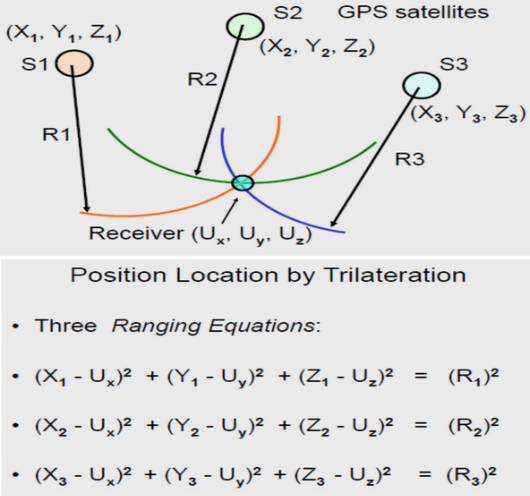
\includegraphics[width = .8\textwidth]{figure/5_8.png}
    \caption{GPS equations}
    \label{fig:gps-equations}
    \end{figure}
    
$X_i$, $Y_i$, and $Z_i$ refer for ith satellite position. \\
$U_x$, $U_y$ and $U_z$ are unknown and they are calculated by solving the three equation, they indicate the receiver position.
 
\subsubsection{GPS Timing}

\begin{itemize}
    \item Each GPS Satellite carries four highly accurate atomic clocks which provide GPS time.
    \item Civil receivers do not have atomic clocks (moderately
     accurate quartz clocks).
     \item Receiver clock must be synchronized to GPS time.
     \item  Requires 4th satellite (fourth equation) to solve for clock bias/error.
     \item Four unknowns are $U_x$, $U_y$, $U_z$, and T.
\end{itemize}

Now, four satellites with four equations are needed to solve timing problem as shown in figure \ref{fig:gps-equationss-time}.

    \begin{figure}[h]
    \centering
    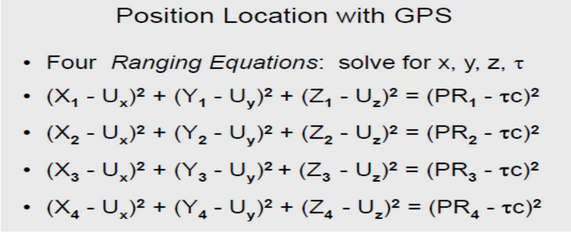
\includegraphics[width = \textwidth]{figure/5_9.png}
    \caption{GPS equations for timing solving}
    \label{fig:gps-equationss-time}
    \end{figure}
 \newpage   
\subsubsection{Receiving GPS data using Bluetooth module}

Bluetooth module communicates with the mobile phone using an Android application called "Share GPS" to get the data as shown in figures \ref{fig:mobile-bt1} and \ref{fig:mobile-bt2}. After successful connection, Bluetooth module shares this data with STM using UART, in next sections configurations and used functions will be discussed.\newpage

\begin{figure}[h]
    \centering
    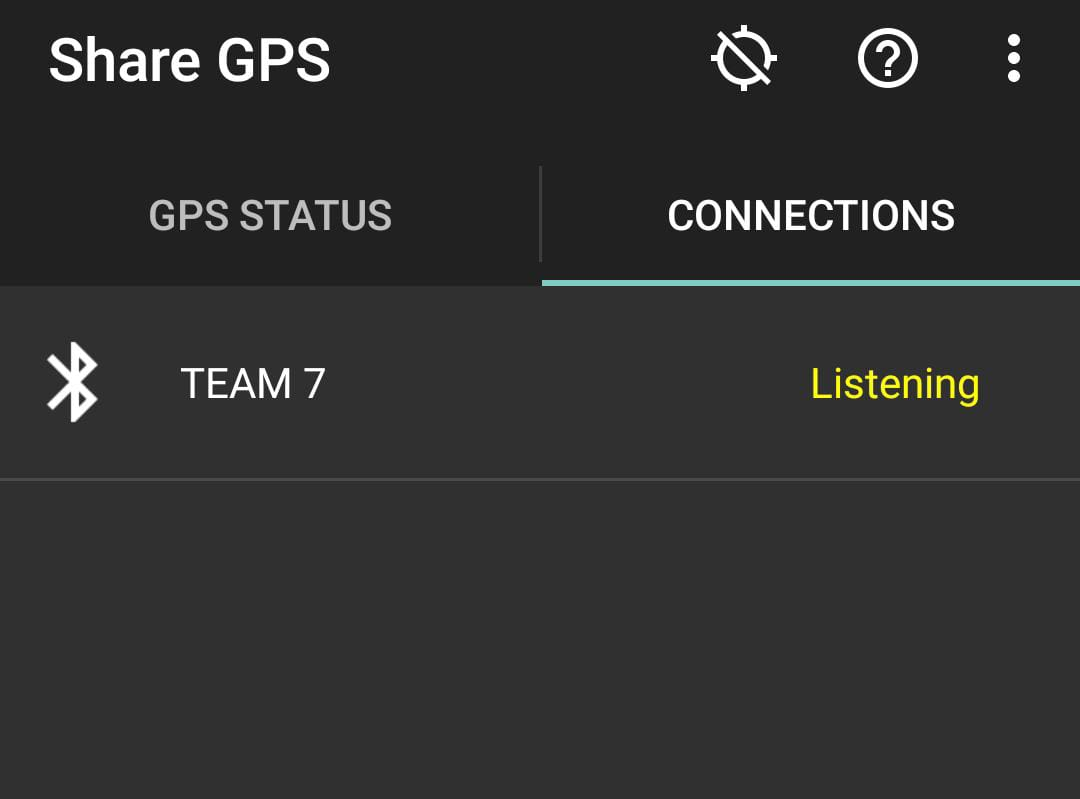
\includegraphics[width = .8\textwidth]{figure/5_10.jpg}
    \caption{Mobile phone is listening to Bluetooth module}
    \label{fig:mobile-bt1}
    \end{figure}
    
\begin{figure}[h]
    \centering
    \includegraphics[width = .8\textwidth]{figure/5_11.jpg}
    \caption{Mobile phone connected to Bluetooth module}
    \label{fig:mobile-bt2}
    \end{figure}
  \newpage  
% \subsubsection{2. Ultra Sonic}
% Ultrasonic used to determine whether or not there is an obstacle ahead and measure
% the distance in small ranges smaller than 1M. \\
% The module used in project is HC-RS04 that connection consist of trig and echo pins ash shown in the figure.

% \begin{figure}[h]
%     \centering
%     \includegraphics[width = \textwidth]{figure/5_12.PNG}
%     \caption{Ultra sonic diagram}
% \end{figure}

\subsection{Configuration Tools}

Bluetooth module needs UART configuration to communicate with the STM, USART3 is configured with NVIC enable as shown in figure \ref{fig:uart-config-bt}.

\begin{figure}[h]
    \centering
    \includegraphics[width = .8\textwidth]{figure/5_13.PNG}
    \caption{UART configuration for Bluetooth module}
    \label{fig:uart-config-bt}
    \end{figure}
 
Enabling NVIC allows usage of UARTRingBuffer library; it is a library that helps in transmitting and receiving data from/to STM By a ring (circular) buffer as shown in figure \ref{fig:uart-ring}  which will be compatible with GPS data since the size of buffer needed for this data isn't constant.

\begin{figure}[h]
    \centering
    \includegraphics[width = .4\textwidth]{figure/5_14.png}
    \caption{UART ring buffer mechanism}
    \label{fig:uart-ring}
    \end{figure}
\newpage 

\subsection{Used functions}

In this section all implemented and used functions will be discussed. \\ First of all, USART3 and ringbuffer are initialized, then the algorithm for the code waits for "RMC" value from GPS, when it's received, the data after it until char '*' will be copied at buffer "RMC", finally \textbf{getGPSData()} is called to get the longitude, latitude, longitude direction, and latitude direction into GPS data structure.\\ RMC command and character '*' will be discussed in chapter 6.

\textbf{The code in main function:}

\begin{lstlisting}

int main()
{
    MX_USART3_UART_Init();
     Ringbuf_init();
    while(1)
    {
        if(Wait_for("RMC") == 1)
	  {
	  	Copy_upto("*", RMC);
	  	getGPSData();

	  }
    }
}

\end{lstlisting}

\subsubsection{getGPSData():}
Going deeply into this function, this function extracts both longitude and latitude neglecting any other received characters (i.e, neglecting ',' character between values), each one is extracted in temporary array to be converted into string using \textbf{atof()} function which is an internal function in C language in which converts array into float number. For directions, they are only one character for them, so they are easy to be extracted and stored in character variables. This implementation must be done when the data is received successfully and the data is valid, this check is done by an if condition in the beginning of the function.

\textbf{getGPSData() part for calculation latitude and latitude direction (this code is the same for longitude data replacing latitude variables with longitude ones):}

\begin{lstlisting}

void getGPSData(void)
{
	while(RMC[indexRMC] == ',') indexRMC++;
	while(RMC[indexRMC] != ',') indexRMC++;

	while(RMC[indexRMC] == ',') indexRMC++;
	gpsData.valid = RMC[indexRMC++];

	if(gpsData.valid == 'V' || gpsData.valid == 'N')
	{
		/* Get latitude */
		indexTempArray = 0;
		tempArray[indexTempArray++] = '0';
		tempArray[indexTempArray++] = '.';
		while(RMC[indexRMC] == ',') indexRMC++;
		while(RMC[indexRMC] != ',')
		{
			if(count == 0)
			{
				if(RMC[indexRMC] == '0') count--;
				gpsData.latitude = (RMC[indexRMC] - '0') * 10;
			}
			else if(count == 1)
			{
				gpsData.latitude += (RMC[indexRMC] - '0');
			}
			else
			{
				if(RMC[indexRMC] != '.')
					tempArray[indexTempArray] = RMC[indexRMC];
				indexTempArray++;

			}
			count++;
			indexRMC++;
		}
		gpsData.latitude += (atof(tempArray) / 60);
		for(globalIndex = 0; globalIndex < 20; globalIndex++)
			tempArray[globalIndex] = '0';
		count = 0;


		/* Get latitude direction */
		while(RMC[indexRMC] == ',') indexRMC++;
		gpsData.dirLatitude = RMC[indexRMC++];


\end{lstlisting}

\subsection{Testing}

The test is done by debugging this variables using STMCube IDE debugger which helps to trace the code line by line.

GPS data structure:
\begin{lstlisting}
typedef struct DataGPS
{
	float longitude;
	float latitude;
	char dirLongitude;
	char dirLatitude;
	char valid;
}gps_t;

\end{lstlisting}

This structure is traced and viewed. To ensure that they are correct values, they are compared with GPS data in the mobile phone, if they are similar then the code works properly. \\

There is a bug in waitfor() function; if it didn't receive RMC, the code will stop in this line infinitely causing error fault. This is done when the power is on, so the STM must be reset when this bug happens.

\section{Sharing-With-Server Unit}
In this section, the discussion will be about how Raspberry Pi and STM exchange data together. Raspberry Pi is chosen due to some features that whill be discussed in next sub-section.

\subsection{Data Collection}

STM and Raspberry Pi communicate with UART protocol to send and receive data that is being shared with the server. Raspberry pi is an efficient IC that has a very strong processor. Although Raspberrpy Pi is expensive compared to other ICs, this is chosen in the project because it will be a suitable component for the applications that will be integrated in the project. Raspberry pi supports GUI, so it will be a good choice for implementing it with the display for showing the data for the user.

\subsubsection{Raspberry Pi features}
\begin{itemize}
    \item 512 MB SDRAM memory.
    \item Broadcom BCM2835 SoC full high definition  multimedia processor.
    \item Dual Core Video Core IV Multimedia coprocessor.
    \item Single 2.0 USB connector.
    \item HDMI (rev 1.3 and 1.4) Composite RCA (PAL & NTSC) Video Out.
    \item 3.5 MM Jack, HDMI Audio Out.
    \item MMC, SD, SDIO Card slot on board storage.
    \item Linux Operating system.
    \item Linux Operating system.
    \item  On board 10/100 Ethernet RJ45 jack.
\end{itemize}
    
\subsubsection{Connecting raspberry with PC}
Raspberry Pi has a linux terminal that can be accessed using a software called "PuTTy" as shown in figure  \ref{fig:putty-config}. By connecting the raspberry with the PC using an Ethernet cable and a USB cable as shown in figure \ref{fig:ether-rasp}, the terminal will be ready on the software and the Raspberry Pi has been successfully accessed. \\

\begin{figure}[h]
    \centering
    \includegraphics[width = .75\textwidth]{figure/5_15.PNG}
    \caption{PuTTy configuration to connect Raspberry Pi with PC}
    \label{fig:putty-config}
    \end{figure}
\newpage 

\begin{figure}[h]
    \centering
    \includegraphics[width = .7\textwidth]{figure/5_16.jpg}
    \caption{Raspberry Pi hardware connection with PC}
    \label{fig:ether-rasp}
    \end{figure}
\clearpage 
\subsubsection{Notes}
\begin{enumerate}
    \item You can access the Raspberry Pi with HDMI screens that will provide you with a full GUI that will be easier to deal with than the Linux terminal.
    \item If the raspberry is too expensive to buy, you can replace it with any IC that provides a Wi-Fi protocol (i.e, ESP32 is suitable).
    \item If there is a problem with opening the terminal in PuTTy, try to allow sharing in adapter options from windows network settings.
\end{enumerate}

Going back to PuTTy, after wiring "raspberrypi.local" in host name then  pressing on "connect", the terminal of Raspberry will be opened and it will be required to enter your user name and password as shown in figure \ref{fig:rasp-terminal}, the default for all raspberries are:
\begin{enumerate}
    \item user name -  pi
    \item password  -  raspberry
\end{enumerate}

    
\begin{figure}[h]
    \centering
    \includegraphics[width = \textwidth]{figure/5_17.PNG}
    \caption{Raspberry Pi terminal for user name and password}
    \label{fig:rasp-terminal}
    \end{figure}
\newpage 

After writing the user name and the password, the operating system opened as shown in figure \ref{fig:rasp-os}, you are now on the home in the raspberry Linux, if you wrote "nano UART.py"command, it will generate this file with python extension. \\
To run UART.py, use "python UART.py" command.
So, python file is written for enable UART for raspberry using serial library. In next sub-section the used python code will be showed.

\begin{figure}[h]
    \centering
    \includegraphics[width = \textwidth]{figure/5_18.PNG}
    \caption{Raspberry Pi operating system terminal}
    \label{fig:rasp-os}
    \end{figure}
\newpage 
    
In next sections, the configuration of STM and used functions in both Raspberry Pi will be discussed.

\subsection{Configuration Tools}

In STMCube, USART2 is enabled as shown in figure \ref{fig:uart-config-rasp}, note that the baud rate changed to 115200 since the raspberry baud rate is 115200, so the two devices must have the same baud rate.

\begin{figure}[h]
    \centering
    \includegraphics[width = \textwidth]{figure/5_19.PNG}
    \caption{UART configuration  in STM for connection with Raspberry Pi}
    \label{fig:uart-config-rasp}
\end{figure}

As will be seen in next sub-section, the functions are in blocking mode, so no need to enable NVIC.

\subsection{Functions Used}
In this section functions used in both raspberry and STM are discussed.

\subsubsection{1. STM}

In the main function the code sequence is written as follow:

\begin{enumerate}
    \item Initialization of UART2 before while loop.\\
    \textbf{Then inside while loop:}
    \item Automatic generated function \textbf{HAL\textunderscore UART\textunderscore Receive()} is called to receive data from the raspberry and store it into a buffer called BufferRX.
    \item \textbf{resetBuffersIndexes()} function is called to reset all indexes before entering in implementation to avoid any garbage error.
    \item \textbf{getNeighborData()} function is called to extract the data received into their suitable variables in neighbor data structure.
    \item \textbf{getCarData()} function is called to extract the data from the sensors into their suitable variables in car data structure.
    \item \textbf{analysis() }function is called to analysis this data, this is will be discussed in details in chapter 6.
    \item \textbf{generateTransmitBuffer()} function in called to insert the values in car data structure into a buffer called be BufferTX.
    \item  Automatic generated function \textbf{HAL\textunderscore UART \textunderscore Transmit()} is called to transmit data stored in BufferTX from the STM to Raspberry Pi.
\end{enumerate}

Going deeply into each manually written functions:

\subsubsection{A. main()}
\begin{lstlisting}
int main()
{
    MX_USART2_UART_Init();
    while(1)
    {
      HAL_UART_Receive(&huart2, bufferRX, sizeof(bufferRX), 0xFFFF);
	  resetBuffersIndexes();
	  getNeighborData();
	  getCarData();
	  analysis();
	  generateTransmitBuffer();
	  HAL_UART_Transmit(&huart2, bufferTX, sizeof(bufferTX), 0xFF);
    }
}
\end{lstlisting}

\subsubsection{B. resetBuffersIndexes()}
\begin{lstlisting}
void resetBuffersIndexes(void)
{
	indexBufferTX = 0;
	indexBufferRX = 0;
}

\end{lstlisting}

\subsubsection{C. getNeighborData()}
\begin{lstlisting}
void getNeighborData(void)
{
	// Get longitude
	neighbor.longitude = splitData();

	// Get latitude
	indexBufferRX++;
	neighbor.latitude = splitData();

	// Get speed
	indexBufferRX++;
	neighbor.speed = splitData();

	// Get Ax
	indexBufferRX++;
	neighbor.Ax = splitData();

	// Get Ay
	indexBufferRX++;
	neighbor.Ay = splitData();

	// Get Angle
	indexBufferRX++;
	neighbor.angle = splitData();

	// Get Vx
	indexBufferRX++;
	neighbor.Vx = splitData();

	// Get Vy
	indexBufferRX++;
	neighbor.Vy = splitData();
}
\end{lstlisting}

\subsubsection{D. getCarData()}
\begin{lstlisting}
void getCarData(void)
{
	car.longitude = gpsData.longitude;
	car.latitude  = gpsData.latitude;
	car.speed     = (float) hrotary.RPM;
	car.Ax        = (float) himu.Ax;
	car.Ay        = (float) himu.Ay;
	car.angle     = 30.001001;
	car.Vx        = car.speed * (sin((car.angle *PI)/180));
	car.Vy        = car.speed * (cos((car.angle *PI)/180));
}
\end{lstlisting}

\subsubsection{E. generateTransmitBuffer()}
\begin{lstlisting}
void generateTransmitBuffer(void)
{
	bufferTX[indexBufferTX++] = 'D';
	bufferTX[indexBufferTX++] = ':';

	mergeData(car.longitude);
	mergeData(car.latitude);
	mergeData(car.speed);
	mergeData(car.Ax);
	mergeData(car.Ay);
	mergeData(car.angle);
	mergeData(car.Vx);
	mergeData(car.Vy);
	bufferTX[indexBufferTX++] = '?';

	for(; indexBufferTX < TX_SIZE; indexBufferTX++)
	{
		bufferTX[indexBufferTX] = '!';
	}
}
\end{lstlisting}

\textbf{splitData()} is used to help in splitting the BufferRx into a separate variables. i.e, BufferRX contains values of speed, acceleration, longitude, latitude,..etc, the function splits these values into their specific variables.

\textbf{mergeData()} is used to help in merging the separate values into BufferTX. i.e, specific variables that represent values of speed, acceleration, longitude, latitude,..etc, the function merges these values into BufferTX.

\subsubsection{splitData()}
\begin{lstlisting}
float splitData(void)
{
	indexTempArray = 0;
	while(bufferRX[indexBufferRX] != ',' && bufferRX[indexBufferRX] != '!')
	{
		tempArray[indexTempArray] = bufferRX[indexBufferRX];
		if(bufferRX[indexBufferRX] == '.') checkInt = 0;
		indexTempArray++;
		indexBufferRX++;
	}
	if(checkInt == 1) tempArray[indexTempArray] = '.';
	checkInt = 1;
	splitValue = atof(tempArray);
	for(globalIndex = 0; globalIndex < 20; globalIndex++)
		tempArray[globalIndex] = '0';
	return splitValue;
}
\end{lstlisting}

\subsubsection{mergeData()}
\begin{lstlisting}
void mergeData(float value)
{

	gcvt(value, TEMP_ARR_SIZE, tempArray);

	for(indexTempArray = 0; indexTempArray < MAX_FLOAT_DIGITS; indexTempArray++)
	{
		if(tempArray[indexTempArray] == '\0') break;
		bufferTX[indexBufferTX] = tempArray[indexTempArray];
		indexBufferTX++;
	}
	bufferTX[indexBufferTX++] = ',';


	for(globalIndex = 0; globalIndex < TEMP_ARR_SIZE; globalIndex++)
		tempArray[globalIndex] = '0';
}

\end{lstlisting}

\subsubsection{2. Raspberry Pi}

In the UART function the code sequence is written as follow:

\begin{enumerate}
    \item Serial library and server libraries are imported.
    \item Size of buffers is initialized.
    \item Message is extracted from JSON file into a string variable, this will be discussed in details in chapter 7.
    \item Adding redundant characters to complete the size of the buffer. \\ \textbf{}{Inside while true loop:}
    \item Data is sent to STM using \textbf{ser.write()}
    \item Data is received from STM using \textbf{ser.read()}
    \item Try catch statement is inserted to avoid any errors in encoding and decoding.
\end{enumerate}

\subsubsection{UART() code: }



\begin{lstlisting}
ser = serial.Serial()
ser.port = '/dev/ttyAMA0'
ser.baudrate = 115200
ser.timeout = 60
ser.open()

TXSize = 50
RXSize = 50
msgReceived = ''

#msgSent = input("Write: ")
msgSent = read_file("test.json")
msgSent = format_json_string(msgSent)
for i in range(len(msgSent), TXSize):
    msgSent += '.'
ser.write(msgSent.encode())
while True:
    msgReceived = ser.read(RXSize)
    try:
        msgReceived.decode()
        print(msgReceived)
        write_json_file("received-test.json", msgReceived)
    except (UnicodeDecodeError, AttributeError):
        print("error")
        pass
    if msgReceived == b'\r':

        break
\end{lstlisting}

UART function is inserted into the main python file that is responsible for running all written code in raspberry, that will be discussed in chapter 8.

\subsection{Testing}
For STM, the testing is done by tracing the code line by line using the debugger in STMCube IDE, it helps for studying the values of each structure continuously, so errors are found out easier. 
For raspberry Pi, printing the message received helps for ensuring that the data received successfully. 

\subsubsection{1. Car Data structure in STM}
\begin{lstlisting}
typedef struct CarData
{
	float longitude;
	float latitude;
	float speed;
	float Ax;
	float Ay;
	float angle;
	float Vx;
	float Vy;
	float dx;
	float dy;
	float x2;
	float y2;
}data_t;
\end{lstlisting}

\subsubsection{2. Printed message on Raspberry Pi}
The message received on STM is displayed as shown in figure \ref{fig:output-rasp}, to ensure that the reception is successful, it is compared with BufferTx in STM and they must be the same. The label for the message is discussed in chapter 6.

\begin{figure}[h]
    \centering
    \includegraphics[width = \textwidth]{figure/5_20.PNG}
    \caption{Output message in Raspberry}
    \label{fig:output-rasp}
    \end{figure}
\newpage 

\subsubsection{Testing Steps}
\begin{enumerate}
    \item UART is tested by only one character.
    \item Test using a manual data.
    \item Test using sensor data.
    \item Test using JSON files.
    \item Test with the server.
\end{enumerate}
\chapter{Analysis and Algorithms}


In order to compare the data from both vehicles and take appropriate action, this chapter demonstrates how a vehicle obtains information about a nearby vehicle and how that information passes from one component to another inside the vehicle.
 
The analyses and procedures used to create this V2V system, as well as the functions needed to program it, will be presented in detail.

\section{Applying laws of motion}
Vehicles are considered as points in a 2D coordinate system as shown in figure \ref{fig:vectors},
they can be connected to the origin point, then vectors laws are applied to them to calculate the distance between these points.
In the rest state, the Cartesian points are known, so applying the distance vector law is possible.
In general, it is rare to use this concept in the project since the main target is to detect distances with variable time during vehicles motion, so motion laws will take the most significant role in the project.
\begin{figure}[h]
    \centering
    \includegraphics{figure/6_1.png}
    \caption{Vectors of vehicles in rest state}
    \label{fig:vectors}
\end{figure}


To apply motion laws, the project needs to measure the car's velocity and acceleration, but due to 2D coordinate system, the analysis must be done in both x and y components, so not only does the project need linearity information, but also it needs the analysis of x and y components for each peripheral, that is why the project uses  an IMU sensor, a rotary encoder, and a compass; as IMU can extract acceleration components directly ($A_x$, $A_y$, and $A_z$), rotary encoder gives information about linear velocity V, compass gives the angle $\theta$ between the vehicle and north direction, by using the angle and the linear velocity, $V_x$ and $V_y$ can be extracted indirectly by $Vsin(\theta)$ and $V cos(\theta)$ respectively as shown in figure \ref{fig:vx-vy}.
\begin{figure}[h]
    \centering
    \includegraphics{figure/6_2.png}
    \caption{$V_x$ and $V_y$ components for vehicle 1}
    \label{fig:vx-vy}
\end{figure}
Now, vehicle information is extracted, and motion laws can be applied, the origin point is the intersection between equator and Greenwich calculated using GPS data, next step is to get position of the vehicle relative to the origin point i.e. (x1, y1).

X coordinate represents longitude values and Y coordinate represents latitude values, this data is extracted from GPS module.

\section{Analysis steps}
\begin{enumerate}
    \item Receive neighbor vehicle data from the server to extract longitude, latitude, speed, angle, speed, and acceleration components for neighbor vehicle.
    \item Extract the vehicle data from sensors.
    \item Using the second law of motion with variable time, both $d_x$ and $d_y$ components for both the main vehicle and neighbor vehicle are calculated as shown:
    \[d_x(t) = \frac{1}{2}A_X t^2 + V_x t\]
    \[d_y(t) = \frac{1}{2}A_Y t^2 + V_y t\]
    \item To calculate $d_x$ and $d_y$ for both vehicles, the processor loops over the equations and substitutes t variable with values from 0 to 10 seconds.
    \item In every loop, the processor calculates  \(d_{xvehicle},    d_{yvehicle}\), $d_{xneighbor}$, and $d_{yneighbor}$, then it determines whether $d_{xvehicle} - d_{xneighbor}$ or \(|d_{yvehicle} - d_{yneighbor}\)
equal to zero, if it is true, this means that the two vehicles will be at the same point after time t and collision has occurred, so the processor must send a warning for the user to prevent this future accident immediately.
    \item The previous calculations treat vehicles as if they were points on a plane, however since vehicles have proper dimensions, threshold values, $D_{xmin}$ and $D_{ymin}$  need to be determined based on the actual dimensions of the vehicles.
    \item After that, the main vehicle data is sent to all neighbor vehicles to be processed in other vehicles.
    \item Finally, the processor resets the neighbor variables to be ready to receive other neighbor data and repeat the analysis steps.
\end{enumerate}

\section{Analysis programming code}
This section shows the analysis idea implementation in the programming, and how to write the analysis steps as program codes.

First, there are two definitions that must be taken into consideration; the first one is connection between V2V unit and other neighbor V2V units, and the second one is connection between components inside each V2V.
The first definition is done by connecting all Raspberry Pis inside all V2V units with the server to send and receive JSON files which contain the vehicles data, the code here is written in Python and the implemented functions were:
\begin{itemize}
    \item Send JSON files to multiple clients: data taken from STM needs to be converted to the standard format JSON and sent to the server which is responsible for broadcasting that file to other vehicles.
    \item Receive JSON files from multiple clients: files coming from the server must be received correctly by the Raspberry Pi in the vehicle and sent to the STM to do the previously explained processing.
\end{itemize}
The mechanism in which this happens will be explained thoroughly in the incoming chapters.

The second definition is done by connecting the Raspberry Pi with the STM using UART protocol, and connecting STM with IMU using I2C protocol, GPS module using UART protocol, and rotary encoder using timer peripheral.
After receiving JSON file, Raspberry Pi converts it into string to be sent to STM, and when STM receives it, STM stores it into buffer RX array. Note that both STM and Raspberry Pi  must have the same declaration for transmit “Tx” buffer size and receive “Rx” buffer size, and this value must indicate the maximum size of the sent and received data, and if the data is less than this value, dummy characters are inserted before sending or receiving.

For example, if the sending data size in Raspberry Pi is 30 characters, and the receiving buffer in STM size is 40 characters, the STM will receive the data and wait for another 10 characters to be received, and this causes overlapping between vehicles data.

Another example, if the data sending size in Raspberry Pi  is 30 characters, and the receiving buffer in STM size is 20 characters, the STM will receive only 20 characters and the remaining characters will be lost.
 
- Raspberry Pi implements some functions for JSON file; \textbf{write\_json\_file} and \textbf{read\_json\_file} and this functionality is defined as follows:

\begin{enumerate}
    \item \textbf{write\_json\_file}: to take string from the Raspberry Pi  and extract the vehicle data (neglecting dummy characters) and convert this string into JSON file, JSON file must contain the data values and the IP address of the Raspberry Pi, so it also inserts the IP address into the JSON file.
    \item \textbf{read\_json\_file}: After receiving a JSON file (all JSON files are now containing IP address and vehicle data), this function extracts the vehicle data and converts it into string, and if the size of the string is less than the Tx buffer size, it inserts a dummy char.
    \item \textbf{UART}: This function uses serial library, and it is responsible for calling \textbf{read\_json\_file} and sending it to STM, then receiving string from STM and calling \textbf{write\_json\_file} to convert it into JSON.
    
\end{enumerate}
Inside while (1) in STM, transmission/reception are done, analysis is calculated, data from sensors is extracted. Code in STM is written by C/Embedded C.

\begin{enumerate}
    \item Transmission and reception between STM and Raspberry Pi:
Once the STM receives data from Raspberry Pi by \textbf{HAL\_UART\_Receive\_IT }function and makes the analysis, it generates the TX buffer to send it to Raspberry Pi using \textbf{HAL\_UART\_Transmit} function.
The analysis is done inside \textbf{HAL\_UART\_RxCpltCallback} function to ensure that all reception is done successfully, and all data is inside RX buffer, and after analysis, \textbf{HAL\_UART\_Transmit} is
also called inside \textbf{HAL\_UART\_RxCpltCallback}.
    \item Analysis after receiving:The data into RX buffer is written in the following format:
“longitude,latitude,speed,Ax,Ay,angle,Vx,Vy,Dummy”
Example:
If the received data was: 

“32.123456,29.435213,34.56, +10.21,-3.22,30.567,20.541,17.823, !!!!!”
This means the following:


\bgroup
\def\arraystretch{1.5}% 
\begin{table}[h]
\centering
\begin{tabular}{| c | c |}
\hline
 Longitude &32.123456 \\
 \hline
 Latitude &  29.435213 \\
 \hline
 Speed & 34.56 \\ 
 \hline
 $A_x$ & +10.21  \\
 \hline
 $A_y$ & -3.22  \\
 \hline
 Angle & 30.567  \\
 \hline
 $V_x$ & 20.541 \\
 \hline
 $V_y$ & 17.823 \\
 \hline
 Dummy Data & !!!!!  \\
 \hline

\end{tabular}
\end{table}
\egroup

\end{enumerate}

The analysis is done by implementing some functions, these functions are:

\begin{enumerate}
    \item \textbf{resetBuffersIndexes}: First, this function is called to ensure that the RX and TX buffers indexes point to the first char inside them.
    \item \textbf{splitData}: It takes some data part (this part may define longitude, latitude,..etc) from the RX buffer and convert it into float number and return it.
    \item \textbf{getNeighborData}: It sets the pointer of the RX buffer which detects some data, then it calls \textbf{splitData}() to get the float number and store it into its specific value, then it repeats setting the RX buffer pointer to get all the peripherals values.
    \item \textbf{getCarData}: It connects with sensor drivers and takes the car data from them.
    \item \textbf{sendWarning}: It is responsible for sending the suitable warning message by inserting the message into the Tx Buffer to be sent with vehicle data.
    \item \textbf{analysis}: It is responsible for applying second motion law over variable time (looping over the time) and compare dx components with $D_{X\_min}$ and $d_y$ components with $D_{Y\_min}$, and if there is a danger, it calls the function \textbf{sendWarning}.
    \item \textbf{mergeData}: It takes a float data (this data may define longitude, latitude,..etc) and convert it into string, then it stores it into TX buffer.
    \item \textbf{generateTransmitBuffer}: This function is responsible for generating the specific format “longitude,latitude,speed,Ax,Ay,angle,Vx,Vy,Dummy” , it calls \textbf{mergeData} for every peripheral, then it inserts dummy characters if it is needed.
\end{enumerate}
Here is how these functions are utilized to correctly perform the analysis:
\begin{itemize}
    \item STM calls the \textbf{HAL\_UART\_Receive\_IT} for receiving neighbor vehicle data into Rx buffer, and when is reception is done, HAL driver calls \textbf{HAL\_UART\_RxCpltCallback} automatically, so that all code is written inside this function to ensure that all neighbor data is inside Rx buffer.
    \item The first function will be called in \textbf{HAL\_UART\_RxCpltCallback} is                  \textbf{resetBuffersIndexes} for initializing the indexes of the buffers to point for the first address in both buffers.
    \item After that, \textbf{getNeighborData} is called to get the neighbor vehicle data from RX buffer and convert it into float numbers and store each value into its specific variable.
    \item Next, \textbf{getCarData} is called to get the main vehicle data from the sensors, it is better to call \textbf{getCarData} after \textbf{getNeighborData} and before analysis since the sensors change variables simultaneously and analysis needs the latest updated values for the peripherals.
    \item After that, \textbf{analysis} is called to apply motion laws and detect any future collision.
    \item Next, \textbf{generateTransmitBuffer} is called to insert the main vehicle data into the Tx buffer. Note that the Tx buffer may also contain a warning message.
    \item Finally, using \textbf{HAL\_UART\_Transmit} is called to transmit both data and warning message (if exists) to Raspberry Pi.
\end{itemize}
Now, the Raspberry Pi receives three kinds of data; warning message, vehicle data, and dummy data. Thus, after receiving is done, Raspberry Pi detects the warning message and displays it on its screen, removes dummy data, and converts the vehicle data into JSON file by \textbf{write\_json\_file} function.




\chapter{V2V Server Implementation}
Reaching a crucial element in the project, the link that the end devices which would be the Wi-Fi network and the server that organizes the messaging between individual cars. This chapter discusses the process of utilizing a Wi-Fi network to alert other cars starting from the very initial tests that leave the server's role in routing the information.

\section{Server}
This part of the network allows the addition of the users on the get go without the need to add them manually on this server as. The server broadcasts the incoming files to the remaining end devices on the network such that each vehicle can make an informed decision about its next move. This begs the question of how it broadcasts the message. First we need to know what a socket is, a socket is a kind of a software structure of a computer network that acts as an endpoint for sending and receiving data across the network. The server utilizes a socket object from the python socket library with the TCP protocol for more reliable messaging as the TCP protocol makes sure of sending or receiving data correctly unlike the UDP protocol which relies on the best effort only. After creating the socket object, the server can receive files from connected clients and send it to the remaining clients.

Before discussing the inner workings of the, it will prove useful to explain a little bit about a design pattern called Observer design pattern. A design pattern is a solution to a common problem. There are several classifications for design patterns, one of them is called behavioral design pattern, they take care of effective communications between objects.

Observer design pattern is a behavioral design pattern that lets you define a subscription mechanism to notify multiple objects about any events that happens to the object they are observing (the observable), in case of the server the observer would be the vehicles and the observable would be the server, when a vehicle sends a file to the observable it would notify the other vehicles. 
\clearpage

\begin{lstlisting}[language=Python]
# Constants
PORT = 5040
SERVER = socket.gethostbyname(socket.gethostname())
ADDRESS = ('192.168.1.5', PORT)
FORMAT = 'utf-8'
 
server = socket.socket(socket.AF_INET, socket.SOCK_STREAM)
server.bind(ADDRESS)
 
def start():
   serverObservable = Observable()
   server.listen()
   print(f"[LISTENING] Server is listening on {SERVER}:{PORT}")
   while True:
       conn, addr = server.accept()
       thread = threading.Thread(
           target=handle_client, args=(conn, addr, serverObservable))
       thread.start()
 
 
print("[STARTING] server is starting...")
start()
\end{lstlisting}
At first comes some constants definitions required to make a socket, then a function called \textbf{start}  is defined as the name indicates responsible for starting the server, in this function the server observable is created, then by executing \textbf{listen} method on the socket object, the server is ready to accept incoming connections from the vehicles, when a vehicle tries to connect to the server, a new thread is created to handle that vehicle and a function called \textbf{handle\_client} is executed.

\clearpage
\begin{lstlisting}[language=Python]
def handle_client(conn, addr, serverObservable):
   print(f"[NEW CONNECTION] {addr} connected.")
   connection_buffer = Buffer(conn)
   serverObservable.subscribe([conn, addr[0]])
   while True:
       file_name = connection_buffer.get_utf8()
       if not file_name:
           break
       full_file_name = os.path.join('files', file_name)
       file_size = int(connection_buffer.get_utf8())
 
       with open(full_file_name, 'wb') as f:
           remaining = file_size
           while remaining:
               chunk_size = BUFFER_SIZE if remaining >= BUFFER_SIZE 
               else remaining
               print(chunk_size)
               chunk = connection_buffer.get_bytes(chunk_size)
               if not chunk:
                   break
               f.write(chunk)
               remaining -= len(chunk)
           if remaining:
               print('File incomplete.  Missing', remaining, 'bytes.')
           else:
               print('File received successfully.')
       file_ip = json.loads(read_file(full_file_name))["ip"]
 
       serverObservable.notify(file_name, file_ip)
   serverObservable.unsubscribe(conn)
   print('Connection closed.')
   conn.close()
\end{lstlisting}

This function does three things, first it adds that vehicle to the subscribers list, second it keeps receiving files incoming from that client and third it notifies other vehicles, notify here means sending received files to them. 

\section{client}
The objective here is to get the data from the other sensors and order it in a readable file for other members of the network to receive it, analyze it and make the decision accordingly.

\subsection{Socket Programming Trial}
First to get a feel of how to use socket programming in python, an echo server was established on a single laptop to understand the working principles. Two files were in the works, the client and the server. The intended mission here is to have the server file listen on the agreed upon port number for a certain message from the client, for example a string “This is the client!”. Once the message is received by the server it is sent back to the client through the same port to be printed on the screen hence the name echo server.

\subsection{Simplex}
Like any communication system starting with the case of the simplex, the client can send a file for a one way street communication case that was tested out and succeeded in sending only one file however when we tried to send multiple files a problem occurred, a bad discriminator error. This problem rose because multiple files were attempted to be sent sequentially. This error is fixed when choosing a buffer solution search that all the files can be put in one buffer then sent all at once.

\subsection{Half Duplex}
Modifications on the simplex code were made such that either the server or the client can send a file at a time.

\subsection{Full Duplex}
The following sections describe how the full duplex came to be.

\subsubsection{Multiple client handling}
With the help of threading each client can be on a different thread such that the server can communicate with multiple users at one time. However threading isn't the only factor to complete this kind of a task, there was a need for an algorithm to administer the process called the Observer Design Pattern. Observer pattern is used when there is one-to-many relationship between objects such as if one object is modified, its dependent objects are to be notified automatically. Observer pattern falls under the behavioral pattern category. In our case the observer is the server and the observable are the clients connected.
\newline\newline
\textbf{Upcoming two sections rely on the library of multiprocesses to make this work}

\subsubsection{UART handling}
As part of the client, the raw data coming from the microcontroller is read serially and organized in a JSON file named after the IP address of the vehicle and sends it over the network to the server. The received files are fed serially into the microcontroller to make an informed decision.

\subsubsection{Server handling}
This part receives the incoming files from the server and puts them in the folder where the UART handler can feed them to the micro-controller.
\chapter{Hardware Implementation}

In the previous chapters each part of the system was explained, but with no information about how all these parts will work together to create the whole project, and that’s what this chapter is about. Communication, not surprisingly, is a role key in any V2V project either that communication is between vehicles and each other, objective of the project, or is between each module of the project.

\section{Embedded with JSON}
As explained previously the project constitutes of two main modules, vehicle unit, or embedded unit and server unit, to each its own goal in the case of embedded unit its purpose is to get various data about the vehicle and send it somehow to the Raspberry Pi, which allow the vehicle unit to communicate with the server therefore other vehicles. Since the goal is to send this data to other vehicles it was a must to package this data in a file, the type of file must be agreed upon, so other clients can extract the data from it successfully.

An interesting type of file that proved useful in this case is called JSON. JSON is a standard file format that uses human readable text to store and transmit data objects consisting of key value pairs, here is an example of JSON file that might be transferred between vehicles:



\begin{lstlisting}
{
	"speed": 60,
	"acceleration": 6
	"ip": 0.0.0.0
}

\end{lstlisting}

Of course data sent from the embedded unit isn’t in this format, so some processing must be done first to convert it to the agreed upon standard, fortunately working with strings is quite easy in Python it’s only a matter of simple string manipulation methods.\\

Data coming from embedded unit consists of two parts, data part and warning part the part that needs to be processed is the data one, a question mark is used to separate between these two parts, in each part there are key value pairs, A function named \textbf{write\_json\_file} is responsible to convert this format to JSON.

\clearpage
\begin{lstlisting}
import json
def write_json_file(file_name, formatted_string):
   """
   Writes a formatted string to a json file.
 
   Parameters
   ----------
   file_name : str
       The name of the file to write to.
   formatted_string : str
       The formatted string to write to the file.
   """
   json_object = {}
   for item in formatted_string.split("?"):
       if item[0] == "D":
           json_object["D"] = item.split(":")[1]
   with open(file_name, 'w') as f:
       f.write(json.dumps(json_object))
\end{lstlisting}

At first an empty dictionary, or object, is created to hold the key value pairs, then it loops over the string coming from STM and splits it over the delimiter, a question mark, to get the part that it’s concerned with, which is the data part, after that it adds each key value pair in this data to the empty dictionary, and finally it writes that dictionary to a json file.

\section{Embedded with server}

After all is said and done, a JSON file with data about the vehicle is created and waiting to be sent to the server which is responsible for broadcasting this file to other connected vehicles.\\

It was mentioned before that the component responsible for communication with the outer world is a Raspberry Pi as its purpose is to send and receive JSON files , but before explaining the mechanism by which that is achieved a problem is starting to rise, the Raspberry Pi is always receiving data from STM and at the same time it’s also receiving JSON files coming from the server so two different processes needs to be always running in order for the Raspberry Pi to achieve its main objective.\\

The two main processes are \textbf{uart\_handler} and \textbf{server\_handler},

\textbf{uart\_handler} is responsible for receiving data coming from STM, converting it to JSON format and sending JSON file to the server.
\clearpage
\begin{lstlisting}
def uart_handler():
   while True:
       receive_from_uart()
       print("Different file!")
       add_ip_address("files_to_be_sent/" + get_ip_address() + ".json")
       send_files(client, [get_ip_address() + ".json"])
\end{lstlisting}

Like it was mentioned before the Raspberry Pi needs to be always receiving and sending files to the STM, another function comes in handy here, \textbf{receive\_from\_uart} is the function that’s responsible for communicating with the STM.
\begin{lstlisting}
def receive_from_uart():
   ser = serial.Serial()
   ser.port = '/dev/ttyAMA0'
   ser.baudrate = 115200
   ser.timeout = 5
   ser.open()
 
   TXSize = 100
   RXSize = 100
   msgReceived = ''
 
   if (len(listdir("received_files")) > 0):
       msgSent = read_file(listdir("received_files")[0])
       msgSent = generate_formatted_string_from_json_string(msgSent)
       for i in range(len(msgSent), TXSize):
           msgSent += '!'
       ser.write(msgSent.encode())
 
   msgReceived = ser.read(RXSize)
   try:
       msgReceived.decode('utf-8')
       if(len(str(msgReceived)) > 3):
           write_json_file("files_to_be_sent/" + get_ip_address() + ".json",
                           str(msgReceived)[2:])
   except (UnicodeDecodeError, AttributeError):
       print("error")
       pass
   if msgReceived == b'\r':
       return
   msgReceived = ''

\end{lstlisting}
\clearpage
\textbf{receive\_from\_uart} does two things, check if there are any files ready to be sent to the STM and if there are it will first convert these JSON files to the format that’s understood by the STM and second it receives the data coming from the stm, convert it to a JSON file with the name of its ip.

Back to the main function that is \textbf{uart\_handler} after data from the STM is received and converted to the right format a key value pair is added to the JSON file that represents the ip of the Raspberry Pi, this key value pair helps the server to avoid sending the file back to the vehicle.

The second main process is called \textbf{server\textunderscore handler}:

\begin{lstlisting}
def server_handler():
   while True:
       receive_from_server(client_buffer)
\end{lstlisting}

Nothing fancy is happening here since most of the hard work is done in the function called \textbf{receive\textunderscore from\textunderscore server}:

\begin{lstlisting}
def receive_from_server(client_buffer):
   file_name = client_buffer.get_utf8()
   file_name = os.path.join('received_files', file_name)
   file_size = int(client_buffer.get_utf8())
 
   with open(file_name, 'wb') as f:
       remaining = file_size
       while remaining:
           chunk_size = BUFFER_SIZE if remaining >= BUFFER_SIZE else remaining
           print(chunk_size)
           chunk = client_buffer.get_bytes(chunk_size)
           if not chunk:
               break
           f.write(chunk)
           remaining -= len(chunk)
       if remaining:
           print('File incomplete.  Missing', remaining, 'bytes.')
       else:
           print('File received successfully.')
\end{lstlisting}

When the file is coming from the server, the first thing that’s sent is the file name, then the file size after that the file content will be sent over multiple chunks of constant size, each time a chunk is received the function checks to see if the file is complete or not.
\clearpage
These two main processes needs to be running in the same time:
\begin{lstlisting}
if __name__ == "__main__":
   p1 = Process(target=uart_handler)
   p1.start()
   p2 = Process(target=server_handler)
   p2.start()
   p1.join()
   p2.join()
\end{lstlisting}

Process is a method provided by multiprocessing library, so with these simple lines of code the Raspberry Pi functionality is complete.

\section{circuitry}
To simulate the project a prototype needed to prove the concept and to preform the proper
adjustments to test the data outputs, process it and to obtain
results.
The approach was to build two identical Robo-cars that can
represent the minimum V2V system, controlling the cars remotely.
\subsection{Motors}
A classic set of geared motor with a working voltage of 9V to 12V
equipped with the IR encoder rotary count disc made the basic motion system
\begin{figure}[h]
    \centering
    \includegraphics[scale=.5]{figures/9-3.png}
    \caption{Motors}
    \label{fig:motors}
\end{figure}
\subsection{Drivers}
to control the direction and speed of the motors, even the direction to preform different set of
motions start and stop the vehicle system needed a set of suitable motor drivers.
a motor driver of choice was the LM298D dual channel H—Bridge motor driver that was cheap yet
capable of doing the assigned task perfectly.
the driver have the function of controlling the speed using PWM signals and have 4 pins that control
the direction of each motor front or back separately.

\begin{figure}[h]
    \centering
    \includegraphics[scale=.5]{figures/9-4.png}
    \caption{Drivers}
\end{figure}


\subsection{Level Shifter}
The STM32 blue pill board uses logic 3.3V outputs while most component uses 5V logic high inputs so,
outputs of the STM32 needed to be shifted up to the 5V level hence using a MOSFET
level shifter solved the problem.

\begin{figure}[h]
    \centering
    \includegraphics[scale=.5]{figures/9-5.jpeg}
    \caption{Level Shifter}
\end{figure}
\clearpage

\begin{figure}[h]
    \centering
    \includegraphics[scale=.5]{figures/9-6.png}
    \caption{Level Shifter Connection}
\end{figure}



\subsection{Bluetooth module}
To control the prototype car remotely, a Bluetooth module was used to receive control signal, using a Bluetooth based remote that can easily found or built –
 even a smart phone considered one – controlling the
car became a simple task.

\begin{figure}[h]
    \centering
    \includegraphics[scale=.3]{figures/9-7.png}
    \caption{Bluetooth Module Connection}
\end{figure}

\clearpage

\subsection{CAN Bus System}
Using CAN protocol which is an industrial standard needed to build its hardware system that consisted of a CAN controller, CAN module and CAN transceiver.

\begin{itemize}
    \item CAN Controller: Hardware wise CAN controller interface task was easy one as it’s already on the stm32-bluepill development board only needed to identify and connect with it’s pins.
    \item CAN Transceiver: CAN TRANSCEIVER used to send and receive CAN signal controlled by the STM 32 controller.
The TRANSCEIVER needed to be designed as it wasn’t found as a module in the local market so starting up with the tja1051t IC the
following circuit was made.
\begin{figure}[h]
    \centering
    \includegraphics[scale=.5]{figures/9-8.png}
    \caption{CAN Transceiver PCB}
\end{figure}

    \item CAN Module: CAN module used to receive the CAN signal in devices we need to control if the
CAN protocol is not hardware implemented on it already.
The module used is MCP-2515.
    \begin{figure}[h]
    \centering
    \includegraphics[scale=.6]{figures/9-9.png}
    \caption{CAN Module PCB}
\end{figure}
\end{itemize}

\section{Prototype}
First, the prototypes must be moving to be able to use them in V2X application by using four dc motors, two L298D motor drivers and one STM32F103C8T6 micro-controller for each prototype (car chassis). Then each assembly car is needed to be integrated with the micro-controller to be able to control it in a wireless method by Bluetooth. After that, Interaction between the assemble car and the project is implemented. Finally, the project is copied into the second assemble car and tests have to be done with the server.\\
In this section, previous steps will be discussed individually.

\subsection{Hardware Drivers}

The L298 is an integrated monolithic circuit in a 15- lead Multiwatt and PowerSO20 packages. It is a high voltage, a high current dual full-bridge driver designed to accept standard TTL logic levels and drive inductive loads such as relays, solenoids, and DC and stepping motors. Two enable inputs are provided to enable or disable the device independently of the input signals. The emitters of the lower transistors of each bridge are connected together and the corresponding external terminal can be used for the connection of an external sensing resistor. An additional supply input is provided so that the logic works at a lower voltage.

\begin{figure}[h]
    \centering
    \includegraphics[scale=.4]{figures/9-10.png}
    \caption{L298D Motor Drivers}
\end{figure}

\begin{figure}[h]
    \centering
    \includegraphics[scale=.5]{figures/9-11.png}
    \caption{L298D Motor Driver Pins}
\end{figure}
\newpage
The assembly car has two floors, Drivers are put in the lower floor as shown in figure \ref{fig:hardware-driver-cars}.

\begin{figure}[h]
    \centering
    \includegraphics[width=.8\textwidth]{figures/9_13.jpg}
    \caption{Hardware Connection of Drivers in the assembly car}
    \label{fig:hardware-driver-cars}
\end{figure}

\subsubsection{Code Configuration}
Drivers need to generate a timer signal for controlling the moving, so in STM the timer is enabled with two channels; each channel in the PWM mode as shown in figure \ref{fig:stm-config}.
\newpage
\begin{figure}[h]
    \centering
    \includegraphics[width=.8\textwidth]{figures/9_14.PNG}
    \caption{STM configuration for Hardware Drivers}
    \label{fig:stm-config}
\end{figure}
Using the timer configuration, moving direction functions are implemented, for each direction there is a function to control it and it is called according to the wireless control. This will be discussed in next sub-section.
\\ \textbf{The implemented functions are:}
\begin{lstlisting}
void Left_Forward(void);
void Right_Forward(void);

void Left_Backward(void);
void Right_Backward(void);

void Left_Stop(void);
void Right_Stop(void);

void Forward(void);
void Backward(void);
void Stop(void);
void Left_Rot(void);
void Right_Rot(void);
void Left_Turn(void);
void Right_Turn(void);

void Speed_Up(void);
void Speed_Down(void);

void Fixed_Speed(void);
\end{lstlisting}
\subsection{Bluetooth Control}
In this subsection the remote control will be discussed and the code that was written to control the car. As said before the Bluetooth module is connected with a Mobile phone to share some data, then it can be connected with a micro-controller by UART to transmit this data to it. The same happened here, Bluetooth module is connected with a mobile phone to get a data from an Android software program called "Bluetooth RC Controller" as shown in figure \ref{fig:rc-bt}.

\begin{figure}[h]
    \centering
    \includegraphics[width=.8\textwidth]{figures/9_15.jpg}
    \caption{RC Bluetooth Controller Software Application}
    \label{fig:rc-bt}
\end{figure}

while pressing on some button, it sends a specific character for Bluetooth module and then it is checked and compared using switch case statement in STM.

\subsubsection{Main function code: }
\begin{lstlisting}
int main(void)
{
	/* USER CODE BEGIN 1 */

	/* USER CODE END 1 */

	/* MCU Configuration--------------------------------------------------------*/

	/* Reset of all peripherals, Initializes the Flash interface and the Systick. */
	HAL_Init();

	/* USER CODE BEGIN Init */

	/* USER CODE END Init */

	/* Configure the system clock */
	SystemClock_Config();

	/* USER CODE BEGIN SysInit */

	/* USER CODE END SysInit */

	/* Initialize all configured peripherals */
	MX_GPIO_Init();
	MX_TIM3_Init();
	MX_USART2_UART_Init();
	/* USER CODE BEGIN 2 */
	HAL_TIM_PWM_Start(&htim3, TIM_CHANNEL_3);
	HAL_TIM_PWM_Start(&htim3, TIM_CHANNEL_4);
	/* USER CODE END 2 */

	/* Infiniteloop */
	/* USER CODE BEGIN WHILE */
	while (1)
	{
		/* USER CODE END WHILE */

		/* USER CODE BEGIN 3 */


		HAL_UART_Receive(&huart2, &CTRL, 1, HAL_MAX_DELAY);
		switch (CTRL)
		{
		case 'F':
			Forward();
			break;

		case 'B':
			Backward();
			break;

		case 'S':
			Stop();
			break;

		case 'L':
			Left_Rot();
			break;

		case 'R':
			Right_Rot();
			break;

		case 'G':
			Left_Turn();
			break;

		case 'I':
			Right_Turn();
			break;

		case 'U':
			Speed_Up();
			sprintf(MSG,"%d\n",Speed);
			HAL_UART_Transmit(&huart2, MSG, 4, HAL_MAX_DELAY);
			break;

		case 'D':
			Speed_Down();
			sprintf(MSG,"%d\n",Speed);
			HAL_UART_Transmit(&huart2, MSG, 4, HAL_MAX_DELAY);
			break;
		}
	}
	/* USER CODE END 3 */
}
\end{lstlisting}

\begin{wrapfigure}{r}{5cm}
    \includegraphics[width=0.5\textwidth]{figures/9_16.PNG}
    \caption{Complete assembly car design}
    \label{fig:complete-assembly}
\end{wrapfigure}
\subsection{Integration With The Project}
After successful remote control, the project was inserted to the assembly car, as said before the assembly car consists of two floors, the project is inserted on the upper floor as shown in figure \ref{fig:complete-assembly}.

\subsection{Project Copying}
After ensuring that all sensors work properly, the project has to be be copied on another assembly car to test between them and make them communicate through the server. Testing the two cars is done by making them move in which they will make an accident and it is expected that the two cars send a warning to be displayed. \\

\textbf{Finally, the basic structure for V2V is implemented and the project is excitedly ready for the applications. } 
\chapter{Applications and Future Improvements}

\section{Applications}

As the purpose of any project or research in engineering is to introduce solutions to real life problems and scenarios, possible V2V applications are provided within the following subsections.

\subsection{Forward collision warning}

The targeted scenarios here are:

\begin{enumerate}
    \item  a car is moving towards a second car in front of it
    \item  a car suddenly stops while having other cars behind it
\end{enumerate}

\begin{figure}[h]
    \centering
    \includegraphics[scale=.7]{figure10/1.png}
    \caption{Forward collision warning}
\end{figure}

In the first scenario the car in the front gets a warning notification while in the second scenario the cars in the rear get the warning notification. This gives the driver enough time to react to avoid collision.
\clearpage
\subsection{Lane change warning}

The working scenario is one car suddenly changes lane, the driver in the targeted lane needs to get a warning notification to avoid a possible accident.\\

\begin{figure}[h]
    \centering
    \includegraphics[scale=.7]{figure10/2.png}
    \caption{Lane change warning}
\end{figure}

These two previous applications are near field application and the two cars are in line of sight. In real life, Light Detection and Ranging (LIDAR) could be used for the driver to sense its neighboring vehicles. But due its high cost, it was implemented in this project using ultra sonic sensor.A future upgrade for this project is to use a better detection system as LIDAR for the neighboring vehicles.

\subsection{Blind spot warning}

At a crossroad, it would be hard to notice a fast moving car. This why detection is crucial.

\begin{figure}[h]
    \centering
    \includegraphics[scale=.5]{figure10/3.png}
    \caption{Motors}
    \label{fig:motors}
\end{figure}

This is near field application, but it is out of sight. To improve the detection of this application, the infrastructure could be used to send data from the streets. If there is a node connected to crossroad gathering information about vehicles in each street, notifying the drivers in case of a speeding car coming from blind spot.
\\

\subsection{Emergency service warning}

Some vehicles require cooperation from other drivers to clear a path for urgent reasons, for example police force, an ambulance, or a firetruck. Sending out a notification to the vehicles in the intended path would help to free a lane for the emergency vehicle to reach its destination as fast as possible.\\

\begin{figure}[h]
    \centering
    \includegraphics[scale=.5]{figure10/4.png}
    \caption{Emergency service warning}
\end{figure}

This application is far field. The data of the emergency vehicle is known using GPS.\\
A future improvement for this application is to use an algorithm to detect the shortest path for the vehicle and manage the vehicles on this path.

\subsection{Left Turn Assist (LTA) and Right Turn Assist (RTA)}
By identifying stationary or slowly moving cars in front of your car, forward collision warning
systems alert you to the possibility of an impending collision. While you are driving, forward
collision warning uses radar, lasers, or cameras to monitor the road ahead. The technology will
alert you to the danger if there is an oncoming collision utilizing lights, beeps, seat vibrations, or
a combination of these. Additionally, certain systems might tighten your seatbelt and pre-charge
your brakes to help you stop as swiftly as possible.
Forward collision warning systems are rapidly being included into many automobiles, along with
other safety features like automated emergency braking. If you don't apply the brakes quickly
enough to avoid an approaching collision, your car will do it for you if it has automated
emergency braking. Even though autonomous emergency braking might not stop every collision,
the technology might assist reduce the severity of one.
\clearpage
\begin{figure}[h]
    \centering
    \includegraphics[scale=.5]{figure10/5.png}
    \caption{Left Turn Assist (LTA) and Right Turn Assist (RTA)}
\end{figure}

\subsection{Traffic Management}
V2X will give vehicles an invisible safety net, and the technology will reinforce and expand the
impact of future traffic control strategies. Future management systems will be able to do
without stationary sensors while still having good situational awareness, consider what would
happen if all of the data points from millions of cars were delivered to a single location.
Transportation administrators might modify traffic light timing and shift traffic to make
rush hour flow more smoothly with so much real-time traffic data.

\subsection{Road Safety}
These applications provide information to drivers about a variety of potential risks and
circumstances that are not immediately obvious. They provide support for both time-critical and
less time-critical applications and are in charge of supplying preventative steps to
prevent/minimize hazards or crashes. By connecting your car to the vehicles and roadside
infrastructure around it, V2X technology is about to transform mobility as we know it. With
increased awareness of every nearby vehicle, including those that lie out of sight, your car will
be able to actively reduce the risk of accidents and improve traffic flow.

\section{Future improvement}

Other possible additions or improvements to the project include

\begin{itemize}
    \item Embedding the firmware over the air (FOTA) to add the ability for the driver to update the firmware of the V2V system wireless
    \item Using machine learning to study the behavior of the neighboring vehicles to predict their movements and to digitally flag reckless drivers on the road for other drivers to keep an eye out.
    \item Upgrade the V2V to become V2X. So, the infrastructure is added to the system (V2I), the network is added to the system (V2N),… etc.
\end{itemize}
\chapter{conclusion}

Although the human race has achieved a lot when it comes to safety measures, there are still a huge number of accidents happening at this exact moment. Driving assistance is an interesting technology that helps to make driving and commuting a much more safe experience and that was the motive for choosing this project. V2V technology in its simplest form allows vehicles to communicate with each other in a safe way, data communication is crucial when it comes to safety, with the right data drivers can avoid deadly accidents.
There are a lot of V2V implementations, to each its own advantages, this implementation's main advantage is its reduced cost.

The system consists of two units:
\begin{itemize}
    \item Vehicle unit: This is the unit that’s concerned with getting data from the vehicle.
    \item Server unit: This is the unit responsible for communication with the outer world.
\end{itemize}


At first An overview of the project structure was given and the units that constitutes project, after that each unit was discussed in detail to figure out how it will be built, the next step was to figure out how these units will communicate with each other to reach harmonious system, once each unit is implemented, the next logical step was to test these units by building a prototype that will show the functionality of the project, after making sure that the project is ready to be used in real world applications, some of these applications were discussed and possible future improvements. 

In the end a simple V2V implementation was built with a server that’s represented by a python program that can run on any computer, a PCB that theoretically can be connected to any vehicle.

\chapter{References}

\begin{itemize}
    \item \href{https://store.fut-electronics.com/products/mcp2515-can-bus-interface-module}{F. Electronics, "Future Electronics Egypt,"
Electronic Components , 18 7 2015. [Online].}
    \item S. Corrigan, "Introduction to the Controller
    Area Network (CAN)," Texas Instruments,
    Texas, 2002.
    \item \href{https://www.totalphase.com/blog/2019/08/5-advantages-of-can-bus-protocol/}{StaffWriter, "TotalPhase," 20 August 2019.
[Online].}
    \item \href{https://www.iso.org/standard/33422.html}{I. 2. 31, " ISO 11898-1:2003," 12 2003.
[Online].}
\item Microchip, Stand-Alone CAN Controller With
SPITM Interface, Chandler,Arizona: Microchip,
2005.
\item P. Semiconductors, TJA1050, Eindhoven,
Netherlands: Philips Semiconductors, 2003.
\item \href{https://www.circuitbasics.com/basics-uart-communication/}{Campbell, Scott. “Basics of UART Communication.” Circuit Basics. Keim, Robert.}
\item "STMicroelectronics Reveals Extreme Low-Power STM32U5 Microcontrollers with
Advanced Performance and Cybersecurity". www.st.com. Retrieved Feb 25, 2021.
\item \href{https://www.st.com/en/microcontrollers-microprocessors/stm32f1-series.html}{STM32 F1 Website; STMicroelectronics.}
\item \href{https://realpython.com/python-sockets/}{Socket Programming in Python (Guide)}
\end{itemize}


\end{document}